\newcommand*{\TeXturedVERSION}{1.5.0} %% TeXtured 2025-08-06
%%%%%%%%%%%%%%%%%%%%%%%%%%%%%%%%%%%%%%%%%%%%%%%%%%%%%%%%%%%%%%%%%%%%%%%
%% NOTE: If you find any issues or have any suggestions, please open %%
%%       an Issue on GitHub: https://github.com/jdujava/TeXtured     %%
%%%%%%%%%%%%%%%%%%%%%%%%%%%%%%%%%%%%%%%%%%%%%%%%%%%%%%%%%%%%%%%%%%%%%%%

%% Enable built-in LaTeX support for PDF/A compliance (must be before `\documentclass`)
\DocumentMetadata{lang=fr, pdfversion=1.7, pdfstandard=A-2u}
\input{preamble/pdfA-compliance/glyphtounicode}

%% NOTE: Choose the desirable page layout version (electronic vs print)
\documentclass[12pt,a4paper]{report}                      % single-side (electronic)
% \documentclass[12pt,a4paper,openright,twoside]{report}  % two-sided (for printing)

%% Set some toggle flags to control some of the document properties
%% Define some toggle flags

\newif\ifFANCY       %% whether to enable some more fancy stylistic choices
\newif\ifWIP         %% whether to enable debug commands, todos, etc.
\newif\ifEXTRAMARGIN %% whether WIP mode has extra right margin
\newif\ifCENSOR      %% whether to censor denoted passages

\FANCYtrue        %% by default, enable fancy features

% \FANCYfalse % disable some of the more fancy stylistic choices
%% NOTE: Comment out the following lines for the final version
\WIPtrue            % THIS IS A WORK-IN-PROGRESS VERSION
% \EXTRAMARGINtrue  % add extra right margin in WIP version (for notes/corrections)
% \LINKBOXESfalse   % disable reference/link boxes for faster compilations
\CENSORtrue         % THIS IS A CENSORED VERSION

%% Preamble - data, packages, macros, and more
%%% Preamble

%% Data about the document, like title, author, etc.
%% Thesis type: bachelor, master, doctoral
\newcommand*{\ThesisType}{master}

%% Thesis title (exactly as in the formal assignment)
\newcommand*{\ThesisTitle}{\TeXtured{} Manual}
%% Plaintext version for PDF metadata, uncomment if needed (defauls to \ThesisTitle)
\newcommand*{\ThesisTitlePlaintext}{TeXtured Manual \TeXturedVERSION}
%% Thesis title (if custom formatting is needed for the title page, defauls to \ThesisTitle)
\newcommand*{\ThesisTitleFront}{
    \ThesisTitle\\
    {\Huge\color{gray}\TeXturedVERSION}
}

%% Author of the thesis
\newcommand*{\ThesisAuthor}{\textcolor{red}{Author's Name}}
%% Plaintext version for PDF metadata, uncomment if needed (defauls to \ThesisAuthor)
\newcommand*{\ThesisAuthorPlaintext}{Author's Name}

%% Year when the thesis is submitted
\newcommand*{\YearSubmitted}{2025}
%% Year of the last revision, uncomment if it is different from \YearSubmitted
% \newcommand*{\YearRevision}{2025}

%% University
\newcommand*{\University}{Charles University}

%% Name of the department or institute, where the work was officially assigned
%% (according to the Organizational Structure of MFF UK in English,
%% or a full name of a department outside MFF)
\newcommand*{\Department}{\textcolor{red}{Name of the Department/Institute}}

%% Is it a Department (katedra), or an Institute (ústav)?
\newcommand*{\DeptType}{Institute}

%% Thesis supervisor: name, surname and titles
\newcommand*{\Supervisor}{\textcolor{red}{Name, Surname, and Titles}}
%% Thesis co-supervisor: name, surname and titles (uncomment if applicable)
% \newcommand*{\CoSupervisor}{Name, Surname, and Titles}

%% Supervisor's department/institute (again according to Organizational structure of MFF)
\newcommand*{\SupervisorsDepartment}{\textcolor{red}{Supervisor's Department/Institute}}

%% Study programme and specialization
\newcommand*{\StudyProgramme}{\textcolor{red}{Study Programme}}

%% Abstract (recommended length around 80-200 words; this is not a copy of your thesis assignment!)
\newcommand*{\Abstract}{%
    \textcolor{red}{Write abstract here.}
}

%% Subject (short description for PDF metadata)
\newcommand*{\Subject}{%
    Write subject here.
}

%% Keywords (about 3-7)
\newcommand*{\Keywords}{%
    \textcolor{red}{Manual, Demo, Draft, WIP}
}
%% Plaintext version for PDF metadata, uncomment if needed (defauls to \Keywords)
\newcommand*{\KeywordsPlaintext}{%
    Manual, Demo, Draft, WIP
}


%% DEBUG: various helper debug goodies
\input{preamble/debug/commands}
\input{preamble/debug/line-numbers}
\usepackage{silence} % filter out unwanted warnings

\WarningFilter{latex}{Marginpar on page} % ignore "Marginpar on page ___ moved"


%% Colors
%% Colors
\usepackage[rgb,table]{xcolor} % color facilities

%% TODO: slightly darker gray color for "optional" words
\definecolor{ChapterNumberColor}{gray}{0.88}
\definecolor{HeaderColor}{gray}{0.35}
\definecolor{HeaderRuleColor}{gray}{0.75}
\definecolor{UrlColor}{RGB}{255,127,100}
\definecolor{CiteColor}{RGB}{127,230,252}

\definecolor{Gray10}{gray}{0.1}
\definecolor{Gray20}{gray}{0.2}
\definecolor{Gray30}{gray}{0.3}
\definecolor{Gray40}{gray}{0.4}
\definecolor{Gray50}{gray}{0.5}
\definecolor{Gray60}{gray}{0.6}
\definecolor{Gray70}{gray}{0.7}
\definecolor{Gray80}{gray}{0.8}
\definecolor{Gray90}{gray}{0.9}

\definecolor{LightGrayFill}{gray}{0.97}


%% Typesetting, figures, tables, etc.
%%% Typesetting, figures, tables, etc.

\ifpdftex % only for pdfLaTeX
    \usepackage[T1]{fontenc} % better support for accented characters
\fi
\usepackage{lmodern}  % Latin Modern fonts
\usepackage{romanbar} % Roman numerals with bars, provides `\Romanbar{...}`

%% Commands for accessing extra Latin Modern fonts
%%     - `sbc` - sans bold condensed
%%     - `sfq` - sans extended
%% https://www.tug.org/pracjourn/2006-1/robertson/robertson.pdf
\NewDocumentCommand{\sbcseries}{}{\sffamily\fontseries{sbc}\selectfont}
\NewDocumentCommand{\sfefamily}{}{\fontfamily{lmssq}\selectfont}
\DeclareTextFontCommand{\textsbc}{\sbcseries}
\DeclareTextFontCommand{\textsfe}{\sfefamily}

%% use slanted shape for emphasis `\emph{...}`, and for nested emphasis use italics
\DeclareEmphSequence{\slshape,\itshape}

\usepackage{microtype}           % improve typography
\DisableLigatures[-]{family=tt*} % disable ligatures in typewriter font
\usepackage{parskip}             % no paragraph indentation
\usepackage{csquotes}            % context-sensitive quotation facilities

%% Enumerate/itemize environments
\usepackage{paralist}   % improved enumerate and itemize
\setdefaultleftmargin{1.87em}{1.7em}{1.5em}{1em}{1em}{1em}
\setdefaultitem{$\bullet$}{\textbullet}{\textasteriskcentered}{\textperiodcentered}
\setdefaultenum{\bfseries (1)}{\bfseries (a)}{\bfseries (i)}{A.}

%% Configuration of figures, tables, captions, ...

%% Use same numbering for figures, tables, and equations
\makeatletter
\let\c@figure\c@table
\let\c@equation\c@table
\makeatother

%%% Graphics
\usepackage{graphicx}   % embedding of pictures
\graphicspath{          % default paths to figures
    {./figures/}
    {./figures/Inkscape/}
    {./frontmatter/img/}
}
%% Macro for appending to the graphics path
\ExplSyntaxOn
\NewDocumentCommand{\appendtographicspath}{m}{
    \tl_if_exist:cF { Ginput@path } { \tl_new:c { Ginput@path } }
    \tl_gput_right:cn { Ginput@path } { #1 }
}
\ExplSyntaxOff

%%% Tables
\usepackage{adjustbox}      % center big tables
\usepackage{array}          % custom column types in tables
\usepackage{booktabs}       % improved horizontal lines in tables

%% Increase default vertical space between rows in tables (default is 1.0)
\renewcommand*{\arraystretch}{1.1}

\IfPackageAtLeastTF{xcolor}{2024-09-29}{}{
    %% HACK: `ninecolors` is needed for `tabularray`, but fails to load with rgb color
    %%       model (before 2024/09/29) -> see https://tex.stackexchange.com/a/614702
    \selectcolormodel{natural}  % temporarily switch to natural color model
    \usepackage{ninecolors}     % now we can load `ninecolors` package
    \selectcolormodel{rgb}      % switch back to RGB color model
}

\usepackage{tabularray}     % advanced LaTeX tables
\usepackage{codehigh}       % verbatim in tables (with `\fakeverb` macro)
\UseTblrLibrary{amsmath, booktabs, siunitx} % load libraries for `tabularray`


%% Does \centering automatically, provides side captions (`\fcapside`) and much more
%% Inspired by the M-21 Institute of Engineering Thermodynamics figure template
\usepackage{floatrow}
\floatsetup{ % for all floats
    footnoterule = none,
    footposition = bottom,
}
\floatsetup[figure]{
    capbesideposition = right,
    capbesidesep = quad,
}

%% If you want to position the caption above the figure, use the following
% \floatsetup[table]{
%     style = plaintop, % caption always above, no matter where \caption is called
% }

%% Set caption width to be the same as the table width
% \floatsetup[longtable]{LTcapwidth=table} % https://tex.stackexchange.com/a/345772/120853

\usepackage{caption}    % customizing captions in floating environments
\usepackage{subcaption}

% \DeclareCaptionLabelSeparator{slash}{~/~} % `␣/␣` between label and caption
\DeclareCaptionLabelSeparator{slash}{\hspace{0.25em}/\hspace{0.25em}} % `␣/␣` between label and caption
\captionsetup{
    format        = plain,  % no hanging indent
    indention     = 0.6em,  % but still slightly indent the caption
    % format        = hang,   % alternative: hanging indent
    font          = small,
    labelfont     = {sf,bf},
    labelsep      = slash,
    labelformat   = simple,
    tableposition = bottom,
    parskip       = .3\baselineskip plus 1pt,
}

\makeatletter
% Make this new length and indent, same length as regular caption indent:
\newlength{\floatfootruleindent}
\setlength{\floatfootruleindent}{\caption@indent}% Set the new length
% A bit hacky; introduce a rule underneath caption if \floatfoot is called:
\renewcommand*{\floatfootskip}{2pt\color{Gray50}\hspace{\floatfootruleindent}\hrulefill}%
\makeatother

\DeclareCaptionFont{ftfont}{%
    \scriptsize%
    \color{Gray60}%
    \sffamily\raggedleft%
}
\captionsetup[floatfoot]{
    footfont=ftfont, % https://tex.stackexchange.com/q/9547/120853
}

%%% You can change the justification of all side-captions here
% \captionsetup[capbesidefigure]{
%     % When using sidecaptions, the linewidth can be rather small and awkward breaks and
%     % many underfull hboxes occur. Therefore, raggedright.
%     justification=raggedright,
% }
%
% \captionsetup[subfigure]{%
%     labelformat=simple,% 'parens' uses parantheses, 'brace' just the right one
%     labelsep=slash,%
%     labelfont={sf,bf},%
%     list=off,% list=off removes subfigures from LoF
% }%
%
% \captionsetup[subtable]{%
%     labelformat=simple,% 'parens' uses parantheses, 'brace' just the right one
%     labelsep=slash,%
%     labelfont={sf,bf},%
%     list=off,% list=off removes subfigures from LoF
% }%

%% Change counter from Arabic number to letter:
\renewcommand*{\theContinuedFloat}{\alph{ContinuedFloat}}


%% Hyperlinks, PDF metadata
%% Hyperlinks, PDF metadata
\usepackage[allowmove]{url}
\usepackage{hyperref}   % clickable links and metadata
\usepackage{nameref}    % cross-referencing by name
\usepackage{bookmark}   % more control over PDF bookmarks

%% Fallbacks for PDF metadata commands
\ProvideExpandableDocumentCommand{\ThesisAuthorPlaintext}{}{\ThesisAuthor}
\ProvideExpandableDocumentCommand{\ThesisTitlePlaintext}{}{\ThesisTitle}
\ProvideExpandableDocumentCommand{\KeywordsPlaintext}{}{\Keywords}

\hypersetup{
    linktoc=all,         % whole entry in TOC is clickable link
    pdfborder={0 0 0},   % to disable borders/frames around links
    pdflinkmargin=1.0pt, % extra link area around the text box (default 1pt)
    citebordercolor=CiteColor,
    linkbordercolor=LinkColor,
    urlbordercolor=UrlColor,
    % PDF metadata
    pdfauthor=\ThesisAuthorPlaintext,
    pdftitle=\ThesisTitlePlaintext,
    pdfsubject=\Subject,
    pdfkeywords=\KeywordsPlaintext,
    pdfcreator={LaTeX with hyperref, and biblatex/biber},
    pdfdisplaydoctitle, % https://tex.stackexchange.com/a/435434/120853
}
\bookmarksetup{
    numbered, % include chapter/section numbers in PDF outline
    open, openlevel=1, % expand bookmarks to level 1 (chapters)
}


%% NOTE: look of references, hyperlinks, and citations is customized
%%       mainly in `preamble/hacks/custom-reference-boxes.tex`


%% Miscellaneous commands/macros
%%% Macros for math symbols

%% Punctuation in math mode
\newcommand*{\eqend}{\,.}
\newcommand*{\eqcomma}{\,,}

%% Equals in given dimension
\NewDocumentCommand{\eqdim}{O{} m}{
    \IfBlankTF{#1}
    {\mathrel{\overset{\mathcolor{black!70}{d\.=\.#2}}{\scalebox{2.8}[1]{\(=\)}}}}
    {\mathrel{\overset{\mathcolor{black!70}{#2}}{\scalebox{#1}[1]{\(=\)}}}}
}
%% Phantom with relation spacing
\NewDocumentCommand{\relphantom}{m}{\mathrel{\phantom{#1}}}
%% Continuation of expression to the next line
\NewDocumentCommand{\graytimes}{}{\mathcolor{gray}{\times}}

% %% (Optional) Automatically use \mathcolor in math mode
% \NewCommandCopy{\textcolorOrig}{\textcolor}
% \RenewDocumentCommand{\textcolor}{O{} m m}{%
%     \ifmmode%
%         \let\colorcmd\mathcolor%
%     \else%
%         \let\colorcmd\textcolorOrig%
%     \fi%
%     \IfBlankTF{#1}{\colorcmd{#2}{#3}}{\colorcmd[#1]{#2}{#3}}%
% }

%% Determinants (use normal position of superscript/subscript)
\AddToHook{cmd/det/after}{\nolimits} % functionally replaces the following 2 lines
% \NewCommandCopy{\olddet}{\det}
% \renewcommand*{\det}{\olddet\nolimits}
\DeclareMathOperator{\Det}{Det}

%% Misc math macros
\NewCommandCopy{\transpose}{\intercal}
\DeclareMathOperator{\vol}{vol}
\DeclareMathOperator{\sgn}{sgn}
\newcommand*{\Id}{\bm{1}}
\newcommand*{\const}{\mathrm{const.}}
\DeclareMathOperator{\Span}{Span}
\DeclareMathOperator{\diag}{diag}
\newcommand*{\bdry}{\partial}
\newcommand*{\disjunion}{\sqcup} % TODO: spacing too small sometimes (in subscripts)
\NewDocumentCommand{\inclusion}{s}{\IfBooleanTF{#1}{\hookleftarrow}{\hookrightarrow}}
\NewDocumentCommand{\surjection}{s}{\IfBooleanTF{#1}{\twoheadleftarrow}{\twoheadrightarrow}}
\NewDocumentCommand{\exchange}{O{\quad}}{\xleftrightarrow{#1}}

%% Imaginary unit and Euler's number
%% inspired by Niklas Beisert
\NewDocumentCommand{\I}{}{\mathring{\imath}}
\NewDocumentCommand{\E}{s}{\IfBooleanTF{#1}{\mathrm{e}}{\mathinner{\mathrm{e}}}}

%% Big O notation (\biggO for centered O)
\NewDocumentCommand{\bigO} {l m}{\fbraces#1{\lparen}{\rparen}                   {O} {#2}}
\NewDocumentCommand{\biggO}{l m}{\fbraces#1{\lparen}{\rparen}{\raisemath{-0.1ex}{O}}{#2}}

%%% Various fields and number sets
\newcommand*{\R}{\mathbb{R}}
\newcommand*{\Z}{\mathbb{Z}}
\let\C\relax % avoid clashes with babel accent command when additional languages are loaded
\newcommand*{\C}{\mathbb{C}}
\newcommand*{\F}{\mathbb{F}}
\newcommand*{\N}{\mathbb{N}}

%% Group/Representation Theory
\DeclareMathOperator{\Hom}{Hom}
\DeclareMathOperator{\Ker}{Ker}
\DeclareMathOperator{\End}{End}
\DeclareMathOperator{\Aut}{Aut}
\DeclareMathOperator{\gl}{\mathfrak{gl}}
\DeclareMathOperator{\GL}{\mathsf{GL}}
\let\sl\relax % override (anyway deprecated) `sl` command
\DeclareMathOperator{\sl}{\mathfrak{sl}}
\DeclareMathOperator{\SL}{\mathsf{SL}}
\DeclareMathOperator{\oo}{\mathfrak{o}}
\DeclareMathOperator{\OO}{\mathsf{O}}
\DeclareMathOperator{\so}{\mathfrak{so}}
\NewDocumentCommand{\SO}{s}{\operatorname{\IfBooleanTF{#1}{\widetilde{\mathsf{SO}}}{\mathsf{SO}}}}
\DeclareMathOperator{\ISO}{\mathsf{ISO}}
\DeclareMathOperator{\spin}{\mathfrak{spin}}
\DeclareMathOperator{\Spin}{\mathsf{Spin}}
\let\U\relax % avoid clashes with babel accent command when additional languages are loaded
\DeclareMathOperator{\U}{\mathsf{U}}
\DeclareMathOperator{\su}{\mathfrak{su}}
\DeclareMathOperator{\SU}{\mathsf{SU}}
\DeclareMathOperator{\Sp}{\mathsf{Sp}}
\newcommand*{\g}{\mathfrak{g}}
\newcommand*{\rankgroup}{\mathsf{r}}

%%% Differential Geometry

\DeclareMathOperator{\Sect}{Sect}
\NewDocumentCommand{\Tangent}{s e{_}}{\IfBooleanTF{#1}{\bm{T}^{*}\mspace{-2mu}}{\bm{T}}\IfValueT{#2}{_{\mspace{-2mu}#2}}}
\NewDocumentCommand{\TSect}{s e{^_}}{\IfBooleanTF{#1}{\mathcal{T}^{*}\mspace{-2mu}}{\mathcal{T}}\IfValueT{#2}{^{#2}}\IfValueT{#3}{_{\mspace{0mu}#3}}\mspace{-2mu}}
\NewDocumentCommand{\Lie}{}{\mathcal{L}}
\DeclarePairedDelimiterX{\Liebracket}[2]{\dblbracketleft}{\dblbracketright}{#1,#2}
% \DeclarePairedDelimiterX{\Liebracket}[2]{\lbrack}{\rbrack}{#1,#2}

\DeclareMathOperator{\Tor}{\mathsf{Tor}}
\NewDocumentCommand{\Riem}{O{}}{\IfBlankTF{#1}{\bm{R}}{\tens{\bm{R}}{#1}}}
\NewDocumentCommand{\Ric}{O{}}{\IfBlankTF{#1}{\bmrm{Ric}}{\tens{\bmrm{Ric}}{#1}}}
\NewDocumentCommand{\Rscalar}{}{\mathcal{R}}

%% Override `physics` package command `\dd` to optionally use bold `d`
\RenewDocumentCommand{\dd}{s O{} m}{
    \mathinner{
        \IfBooleanTF{#1}{\bm{\mathrm{d}}}{\mathrm{d}}^{\mspace{-1mu}#2}#3
    }
}
%% Bold differential
\NewCommandCopy{\dotunderaccent}{\d}
\RenewDocumentCommand{\d}{O{} m}{\TextOrMath{\dotunderaccent{#2}}{\dd*[#1]{#2}}}


%% Covariant derivative (with optional arguments for space tweaking)
\NewDocumentCommand{\cder}{s O{a} e{_}}{
    \IfBooleanT{#1}{\mspace{-2mu}} % use starred variant when more \cder after each other
    \bm{\nabla}
    \IfValueT{#3}{             % when subscript index is given
        _{                     % start subscript
            \mspace{-7mu}      % remove extra space after nabla
            \chphantom{#3}{#2} % print #3 with the width of #2
        }
    }
}
%% Coordinate derivative
\NewDocumentCommand{\del}{s}{\IfBooleanTF{#1}{\partial}{\bm{\partial}}}
\NewDocumentCommand{\fdel}{O{} m}{{\frac{\del #1}{\del #2}}}
\NewDocumentCommand{\Dv}{O{} m}{{\frac{\bmrm{D} #1}{\mathrm{d} #2}}}
\NewDocumentCommand{\Laplacian}{}{\triangle}
\NewDocumentCommand{\dAlembertian}{s}{
    \mathord{\raisemath{0.07ex}{
            \mspace{1.5mu}
            \IfBooleanTF{#1}{\square[0.35em][boxframe=0.05em]}{\square[][boxframe=0.06em]}
            \.\.
        }}
}
% \RenewDocumentCommand{\dAlembertian}{s}{\mathord{\raisemath{-0.05ex}{\oldsquare}}}

%%% Tweaking of math index positioning, spacing, etc.
%%% (also definitions of new arrows, etc.)

%% TODO: see if \cramped{...} could be used sometimes to make
%%       (inline) math prettier (to avoid weird line spacing weird)

%% Modify size of `\bigwedge`/`\bigodot` and the position of their superscripts
\NewDocumentCommand{\Ext}{e{^}}{
    \scalerel*{\bigwedge}{\xmathstrut[-0.1]{0.1}} % scale down the \bigwedge a bit
    \IfValueT{#1}{^{\mspace{-2mu}#1}} % shift possible superscript little bit to the left
}
\NewDocumentCommand{\Odot}{e{^}}{
    \scalerel*{\bigodot}{\xmathstrut[-0.1]{0.1}} % scale down the \bigodot a bit
    \IfValueT{#1}{^{\mspace{-0mu}#1}} % (do not) shift possible superscript little bit to the left
}

%% Exchange \epsilon and \varepsilon
\NewCommandCopy{\oldepsilon}{\epsilon}
\NewCommandCopy{\oldvarepsilon}{\varepsilon}
\renewcommand*{\epsilon}{\oldvarepsilon}
\renewcommand*{\varepsilon}{\oldepsilon}

%% Math version of `\raisebox` and `\scalebox`
\NewDocumentCommand{\raisemath}{m}{\mathpalette{\raisemathAux{#1}}}% \raisemath{<len>}{...}
\NewDocumentCommand{\raisemathAux}{mmm}{\raisebox{#1}{\(#2#3\)}}
\NewDocumentCommand{\scalemath}{m O{}}{\mathpalette{\scalemathAux{#1}[#2]}}% \scalemath{<factor>}{...}
\NewDocumentCommand{\scalemathAux}{m O{} mm}{\IfBlankTF{#2}{\scalebox{#1}{\(#3#4\)}}{\scalebox{#1}[#2]{\(#3#4\)}}}

%% Modify subscript position
\NewDocumentCommand{\lowerindex}{O{0pt} O{0pt} e{_^}}{
    \IfValueT{#3}{_{\raisemath{#1}{#3}}}
    \IfValueT{#4}{^{\raisemath{#2}{#4}}}
}

%% Modify superscript/subscript positions for some greek letters
\NewCommandCopy{\oldchi}{\chi}
\renewcommand*{\chi}{\oldchi\lowerindex[-1.5pt]}
\NewCommandCopy{\olddelta}{\delta}
\renewcommand*{\delta}{\olddelta\lowerindex[1pt][1.0pt]}
\newcommand*{\bmdelta}{\bm{\olddelta}\lowerindex[1pt][1.0pt]}
\newcommand*{\altdelta}{{\olddelta\xmathstrut[-0.2]{0.0}}}
\newcommand*{\altbmdelta}{{\bm{\olddelta}\xmathstrut[-0.2]{0.0}}}

%% Smaller \in, \notin, \subset, ...
%% https://tex.stackexchange.com/questions/34393/the-mysteries-of-mathpalette
\NewDocumentCommand{\smallermath}{O{0.05ex} O{0.85} m}{\raisemath{#1}{\scalemath{#2}{#3}}}
\newcommand*{\smallplus}  {\mathrel{\smallermath{+}}}
\newcommand*{\textplus}   {\ensuremath{\.\smallplus\.}}
\newcommand*{\smallin}    {\mathrel{\smallermath{\in}}}
\newcommand*{\smallnotin} {\mathrel{\smallermath{\notin}}}
\newcommand*{\smallsubset}{\mathrel{\smallermath{\subset}}}
\newcommand*{\smallotimes}{\mathbin{\smallermath[0ex]{\oldotimes}}}
% \newcommand*{\smallotimes}{\.\smallerrel{\oldotimes}\.}


%% Fix spacing of \left( .. \middle| .. \right)
\NewCommandCopy{\leftOrig}{\left}
\NewCommandCopy{\rightOrig}{\right}
\NewCommandCopy{\middleOrig}{\middle}
\renewcommand*{\left}{\mathopen{}\mathclose\bgroup\leftOrig}
\renewcommand*{\right}{\aftergroup\egroup\rightOrig}
\RenewDocumentCommand{\middle}{sm}{\IfBooleanTF{#1}{\.\middleOrig#2\.}{\mathrel{}\middleOrig#2\mathrel{}}}
\NewDocumentCommand{\innermiddle}{m}{\mathinner{}\middleOrig#1\mathinner{}}

%% Less space around \setminus (\mathord instead of \mathinner)
\DeclareMathSymbol{\setminus}{\mathord}{symbols}{"6E}

%% Redefine `\square` to Young tableaux
\usepackage{ytableau}           % Young Tableaux
\ytableausetup{centertableaux}
\NewCommandCopy{\oldsquare}{\square}
\NewCommandCopy{\oldotimes}{\otimes}
\RenewDocumentCommand{\square}{O{0.55em} O{} O{}}{%
    \IfBlankTF{#1}{\ytableausetup{boxsize=0.55em}}{\ytableausetup{boxsize=#1}}%
    \ytableausetup{aligntableaux=top, boxframe = normal, #2}%
    \operatorname{\ydiagram[#3]{1}}%
}
\NewDocumentCommand{\smallsquare}{O{0.35em}}{\square[#1]}

%% Sizeable bullet
\NewDocumentCommand{\sbullet}{O{0.5}}{%
    \mathbin{\ThisStyle{\vcenter{\hbox{\scalebox{#1}{\(\SavedStyle\bullet\)}}}}}
}
\NewDocumentCommand{\fdot}{}{\mathcolor{black!80}{\sbullet[0.65]}}
\NewDocumentCommand{\adot}{}{\sbullet[0.52]}
\NewDocumentCommand{\idot}{s}{\mathcolor{darkgray}{\IfBooleanTF{#1}{\.\sbullet[0.4]\.}{\sbullet[0.4]}}}

%% (abstract) index placeholders
\NewDocumentCommand{\aind}{}{\bullet}
\NewDocumentCommand{\dind}{}{\mathcolor{black!60}{\sbullet[1.2]}}
\NewDocumentCommand{\ind}{}{\mathcolor{lightgray}{\bullet}}

%% Argument placeholder
\newsavebox{\argumentbox}
\sbox{\argumentbox}{%
    \begin{tikzpicture}[baseline=-0.6ex]
        \node(char)[draw, shape=rectangle, dash=on 1.2pt off 1.05pt phase 0.5pt, dash expand off,
            inner ysep=2pt, inner xsep=2pt, minimum size=0.6em, rounded corners=2pt] {};
    \end{tikzpicture}%
}
\NewDocumentCommand{\argument}{o}{%
    \IfValueTF{#1}{% use #1 as a scaling factor, resizebox relative to the text size
        \scalebox{#1}{\resizebox{!}{0.58em}{\usebox{\argumentbox}}}
    }{% choose scaling factor based on display/text/script/scriptscript math style
        \mathchoice{\argument[1.0]}{\argument[1.0]}{\argument[0.7]}{\argument[0.6]}
    }%
}

%% Curly arrows
\tikzset{
    leadsto/.style={-{Stealth[length=0.6em,open,round]},decorate,decoration={snake,amplitude=0.20ex,segment length=0.5em,pre length=0.2em,post length=0.6em}},
    toleads/.style={{Stealth[length=0.6em,open,round]}-,decorate,decoration={snake,amplitude=0.20ex,segment length=0.5em,pre length=0.6em,post length=0.2em}},
    correspondsto/.style={{Stealth[length=0.6em,open,round]}-{Stealth[length=0.6em,open,round]},decorate,decoration={snake,amplitude=0.20ex,segment length=0.5em,pre length=0.7em,post length=0.7em}},
}
\NewDocumentCommand{\longleadsto}{s O{} O{}}{%
    \ensuremath{\mathrel{
            \tikz[baseline=-0.5ex, inner sep=0ex, font=\scriptsize]{
                \node[minimum width=2.15em, inner xsep=0.6em, align=center] (a){\hphantom{#2}\\[0ex]\hphantom{#3}};
                \IfBlankF{#2}{\node[inner sep=0.3ex, above=0.3ex, xshift=-0.1em] at (a){#2};}
                \IfBlankF{#3}{\node[inner sep=0.3ex, below=0.3ex, xshift=-0.1em] at (a){#3};}
                \IfBooleanTF{#1}
                {\draw[line width=0.6pt, toleads] (a.west) -- (a.east);}
                {\draw[line width=0.6pt, leadsto] (a.west) -- (a.east);}
            }
        }}%
}
%% https://tex.stackexchange.com/questions/170092/xleftrightarrows-command-in-tikz-with-arrows-matching-the-latex-font?rq=1
\NewDocumentCommand{\correspondsto}{O{}O{}}{%
    \ensuremath{\mathrel{
            \tikz[baseline=-0.5ex, inner sep=0ex, font=\scriptsize]{
                \node[minimum width=3.48em, inner xsep=0.8em, align=center] (a){\hphantom{#1}\\[0ex]\hphantom{#2}};
                \IfBlankF{#1}{\node[inner sep=0.3ex, above=0.3ex] at (a){#1};}
                \IfBlankF{#2}{\node[inner sep=0.3ex, below=0.3ex] at (a){#2};}
                \draw[line width=0.6pt, correspondsto] (a.west) -- (a.east);
            }
        }}%
}

%% Quotient macro
\NewDocumentCommand{\bigslant}{O{0.2}O{1.7}mm}{
    \left.\mspace{-1mu}\raisemath{#1em}{#3}
    \mspace{-#2mu} \middleOrig/ \mspace{-\fpeval{#2+1}mu}
    \raisemath{-#1em}{#4} \mspace{-\fpeval{5*#1}mu} \right.
}
% \NewDocumentCommand{\coset}{O{0.05} O{0.1} m m}{\bigslant[#1][#2]{#3}{#4}}
\NewDocumentCommand{\coset}{O{}O{} m m}{#3/#4}
\NewDocumentCommand{\gt}{}{\bigslant{\g}{\mathfrak{t}}}
\NewDocumentCommand{\gts}{}{\bigslant[0.15]{\scriptstyle\g}{\scriptstyle\mathfrak{t}}}
\NewDocumentCommand{\onehalf}{}{\mspace{-2mu}\bigslant[0.15]{\scriptscriptstyle 1 \mspace{-1.2mu}}{\scriptscriptstyle 2}}

%% Cancel macro
\definecolor{cancelgray}{gray}{0.85}
\tikzset{
    main node/.style={inner sep=0,outer sep=0},
    label node/.style={inner sep=0.3em,font=\tiny,overlay},
    strike out/.style={shorten <=-.2em,shorten >=-.2em,overlay,thick,double distance = 0em,line cap=round},
}
\NewDocumentCommand{\cancel}{O{cancelgray}mo}{%
    \tikz[baseline=(N.base)]{
        \node[main node](N){\(#2\)};
        \IfValueT{#3}{\node[label node, gray, anchor=south] at (N.north){#3};}
        \draw[strike out, #1]  (N.south west) -- (N.north east);
    }
}

%% Macros for - links to packages, and verbatim macros for LaTeX commands
%%            - verbatim macros for commands defined specifically by TeXtured

%% will also utilize styles defined in `/preamble/hacks/custom-reference-boxes.tex`
\usepackage{tcolorbox}
\tcbset{
    packagebox/.style ={bottom=0.20ex, fontupper=\ttfamily},
    filebox/.style ={colframe=black!70!cyan!35, colback=black!10!cyan!3, bottom=0.20ex, fontupper=\ttfamily},
    dirbox/.style ={colframe=black!80!cyan!40, colback=black!60!cyan!8, bottom=0.20ex, fontupper=\ttfamily},
    macrobox/.style ={colframe=black!15, colback=black!3, bottom=0.20ex, fontupper=\ttfamily},
    custommacrobox/.style ={colframe=black!25!green!25, colback=black!5!green!5, bottom=0.20ex, fontupper=\ttfamily},
}

\NewTCBox{\packagebox}{!O{}}{link,hrefbox,packagebox,#1}
\NewTCBox{\filebox}{!O{}}{link,filebox,#1}
\NewTCBox{\dirbox}{!O{}}{link,dirbox,#1}
\NewTCBox{\macrobox}{!O{}}{link,macrobox,#1}
\NewTCBox{\custommacrobox}{!O{}}{link,custommacrobox,#1}

\ifLINKBOXES\else
    \RenewDocumentCommand{\packagebox}{O{} m}{\texttt{#2}}
    \RenewDocumentCommand{\filebox}{O{} m}{\texttt{#2}}
    \RenewDocumentCommand{\dirbox}{O{} m}{\texttt{#2}}
    \RenewDocumentCommand{\macrobox}{O{} m}{\texttt{#2}}
    \RenewDocumentCommand{\custommacrobox}{O{} m}{\texttt{#2}}
\fi

\NewDocumentCommand{\package}{m}{%
    % \href{https://texdoc.org/pkg/#1}
    \hrefold{https://ctan.org/pkg/#1}{%
        \packagebox[right=0.1em]{#1\textsuperscript{\tiny\(\,\to\,\)\textsf{CTAN}}}%
    }%
}
\NewDocumentCommand{\fileTeXtured}{O{-0.9\baselineskip} m}{
    \marginpar{
        \vspace{#1}
        \hspace{-\marginparsep}%
        \llap{%
            \filebox{#2}%
        }%
    }
}
\NewDocumentCommand{\dirTeXtured}{O{-1.3\baselineskip} m}{
    \marginpar{
        \vspace{#1}
        \hspace{-\marginparsep}%
        \llap{%
            \dirbox{#2}%
        }%
    }
}

\NewDocumentCommand{\macro}{O{}v}{\macrobox[#1]{#2}}
\NewDocumentCommand{\fakemacro}{O{}m}{\macrobox[#1]{\fakeverb{#2}}}
\NewDocumentCommand{\custommacro}{O{}v}{\custommacrobox[#1]{#2}}
\NewDocumentCommand{\fakecustommacro}{O{}m}{\custommacrobox[#1]{\fakeverb{#2}}}

%%% TikZ, and other drawing packages

\usepackage{tikz}
\usetikzlibrary{
    fadings,
    arrows.meta,
    calc,
    cd,
    decorations.pathmorphing, decorations.markings,
    trees,
    fit, matrix,
}

%% Directory Tree Structure
\tikzset{
    dirtree/.style={ % http://www.texample.net/tikz/examples/filesystem-tree/
        draw=black!80!cyan!40, thick, rounded corners=0.2em,
        growth parent anchor=west,
        grow via three points={one child at (1.0,-0.78) and
            two children at (1.0,-0.78) and (1.0,-1.56)},
        edge from parent path={([xshift=1.2em]\tikzparentnode.south west) |- (\tikzchildnode.west)},
        every node/.style={text=black, anchor=west, inner sep=0.7ex, draw=black!70!cyan!35, fill=black!10!cyan!3, text depth=.25ex, execute at begin node=\vphantom{Aj}},
        directory/.style={draw=black!80!cyan!40, fill=black!60!cyan!8},
        font=\ttfamily,
    },
}

%%% Quiver macros (for https://q.uiver.app/ diagrams)
%% A TikZ style for curved arrows of a fixed height, due to AndréC.
\tikzset{curve/.style={settings={#1},to path={(\tikztostart)
    .. controls ($(\tikztostart)!\pv{pos}!(\tikztotarget)!\pv{height}!270:(\tikztotarget)$)
    and ($(\tikztostart)!1-\pv{pos}!(\tikztotarget)!\pv{height}!270:(\tikztotarget)$)
    .. (\tikztotarget)\tikztonodes}},
    settings/.code={\tikzset{quiver/.cd,#1}
        \def\pv##1{\pgfkeysvalueof{/tikz/quiver/##1}}},
    quiver/.cd,pos/.initial=0.35,height/.initial=0}

%% TikZ arrowhead/tail styles.
\tikzset{tail reversed/.code={\pgfsetarrowsstart{tikzcd to}}}
\tikzset{2tail/.code={\pgfsetarrowsstart{Implies[reversed]}}}
\tikzset{2tail reversed/.code={\pgfsetarrowsstart{Implies}}}
%% TikZ arrow styles.
\tikzset{no body/.style={/tikz/dash pattern=on 0 off 1mm}}

%% Custom equal sign style - https://tex.stackexchange.com/a/443023
\tikzset{
    double line with arrow/.style args={#1,#2}{decorate,decoration={
        markings,%
        mark=at position 0 with {
            \coordinate (ta-base-1) at (0,1.2pt);
            \coordinate (ta-base-2) at (0,-1.2pt);
        },
        mark=at position 1 with {
            \draw[#1] (ta-base-1) -- (0,1.2pt);
            \draw[#2] (ta-base-2) -- (0,-1.2pt);
        }
    }},
    Equal/.style args={#1}{-,double line with arrow={{-,#1},{-,#1}}},
}

%% Inkscape figures
%% https://mirrors.nic.cz/tex-archive/info/svg-inkscape/InkscapePDFLaTeX.pdf
%% this is (and a lot more) already implemented in `svg` package, but no reason to use it
%% TODO: disable this for ArXiv submission (probably just leaving SVGs out will work fine)
\usepackage{shellesc}
\usepackage{filemod}
\NewDocumentCommand{\exportInkscapeSVG}{O{./figures/Inkscape/} m}{%
    \filemodCmp{#1#2.pdf}{#1#2.svg}{}{% regenerate PDF+LaTeX code if SVG is newer
        \ShellEscape{#1inkscape-export-to-latex "#1#2"}% use `inkscape-export-to-latex` script in the same directory
    }%
}
%% the third argument is the name of the SVG file without the extension
\NewDocumentCommand{\includeInkscapeSVG}{O{0.8\linewidth} O{./figures/Inkscape/} m}{%
    \exportInkscapeSVG[#2]{#3}%
    \def\svgwidth{#1}% set the width of the figure
    \input{#2#3.pdf_tex}%
}


%% Layout of the document, formatting of chapters, sections, TOC, etc.
%%% Page dimensions
%% single-side (electronic) -> use `\documentclass[12pt,a4paper]{report}`
%% two-sided (for printing) -> use `\documentclass[12pt,a4paper,twoside,openright]{report}`
\usepackage{geometry} % flexible interface for adjusting page layout/dimensions
\makeatletter
\if@twoside%
    \setlength\Gm@bindingoffset{15mm} % binding offset for two-sided printing
\fi%
\makeatother
\geometry{
    width=145mm,
    height=250mm,
    hmarginratio=1:1,   % space ratio between left and right margins
    vmarginratio=3:4,   % space ratio between top and bottom margins
    includehead,        % include header in total height
    headheight=2.5em,   % height of the header (includes space below the rule)
    headsep=0mm,        % no extra space between header and text
    % showframe,          % for DEBUG: helper lines for adjusting layout
}
\ifWIP\ifEXTRAMARGIN
        \geometry{
            paperwidth=260mm,   % PDF will be wider
            paperheight=297mm,  % A4 paper height
            layoutwidth=210mm,  % Real A4 content area
            layoutheight=297mm,
            layoutoffset=0mm,   % Align A4 layout to left edge
            % showcrop,
        }
        \usepackage{pict2e}
        \AddToHook{shipout/background}{% add gray line indicating the usual paper size
            \color{black!10}\linethickness{0.4pt}
            \put(210mm,0){\line(0,-1){297mm}}
        }
    \fi\fi

%% try to make text on all pages have the same height (default for `twoside`)
\flushbottom

%% Page numbering style and counters for different parts of the document
\makeatletter
\NewDocumentCommand{\frontmatter}{}{     % the front matter
    \pagenumbering{arabic}               %   arabic page numbering from the very first page
    \setcounter{page}{1}                 %   ensure the document starts at page 1
    \gdef\thechapter{\@Alph\c@chapter}   %   uppercase roman chapter numbering
}
\NewDocumentCommand{\mainmatter}{}{      % the main matter
    \cleardoublepage                     %   start on the right page
    \setcounter{chapter}{0}              %   reset chapter counter
    \setcounter{section}{0}              %   reset section counter
    \gdef\thechapter{\@arabic\c@chapter} %   arabic chapter numbering
}
\NewDocumentCommand{\backmatter}{}{      % the back matter (continue with arabic page numbering)
    \bookmarksetup{startatroot}          %   reset bookmarks level (in case parts are used)
    %% BUG: following line does not work as expected (adds space too late)
    % \addtocontents{toc}{\vspace{2ex}}    %   add some space after last part in TOC
}
\makeatother

%%% Headers and footers, page styles
\usepackage{fancyhdr}       % custom headers and footers
% \usepackage{extramarks}     % extra marks for headers and footers

%% Disable `fancyhdr` warning: "\fancyhead's `E' option without twoside option is useless.
%%                               Please consider using the `twoside' option"
\makeatletter
\def\f@nch@fancyhf@Echeck#1{}
\makeatother

\newlength{\headerpadding}  % left/right padding of header
\setlength{\headerpadding}{2pt}
% \RenewDocumentCommand{\chaptermark}{m}{\markboth{\chaptername\ \thechapter.\ #1}{\chaptername\ \thechapter.\ #1}}
% \RenewDocumentCommand{\sectionmark}{m}{\markright{\thesection.\ #1}}

%% Style of the header rule and decorations
\tikzset{
    header rule/.style={HeaderRuleColor,line width=0.9},
    header decor left/.style={HeaderRuleColor,line width=1.0,{Diamond[open]}-,overlay},
    header decor right/.style={HeaderRuleColor,line width=1.0,-{Diamond[open]},overlay},
}

%% Default header style (includes a rule with decorations)
\fancypagestyle{header}{
    \renewcommand*{\headrule}{
        % \renewcommand*{\headrulewidth}{0.9pt}
        % \textcolor{HeaderRuleColor}{\rule[1em]{\headwidth}{\headrulewidth}}%
        \tikz[baseline=-1em]{
            \fill[header rule] (0, 0) rectangle (\headwidth, 0.9pt);
            \ifFANCY % add fancy decorations
                \draw[header decor right] (\headwidth,0.45pt) -- ++(7pt,0);
                \draw[header decor left] (-7pt,0.45pt) -- (0,0.45pt);
            \fi
        }
    }
    \fancyhead[LO]{\hspace{\headerpadding}\textcolor{HeaderColor}{\textsf{\nouppercase{\leftmark}}}}
    % \fancyhead[LO]{\hspace{\headerpadding}\textcolor{HeaderColor}{\textsf{\nouppercase{\rightmark}}}}
    \fancyhead[RE]{\textcolor{HeaderColor}{\textsf{\nouppercase{\rightmark}}}\hspace{\headerpadding}}
    \fancyhead[RO]{\textbf{\thepage}\hspace{\headerpadding}}
    \fancyhead[LE]{\hspace{\headerpadding}\textbf{\thepage}}
    \ifWIP % show draft watermark in footer
        \fancyfoot[C]{\vskip1ex\relax \ttfamily\textcolor{black!15}{Draft - \today}}
    \else
        \fancyfoot{}
    \fi
}
%% For chapter pages, the `plain` style is used
\fancypagestyle{plain}[header]{
    \renewcommand*{\headrule}{
        \hfill\tikz[baseline=-1em]{
            \fill[header rule, path fading=west] (0, 0) rectangle (0.45\headwidth, 0.9pt);
            \ifFANCY % add fancy decorations
                \draw[header decor right] (0.45\headwidth,0.4pt) -- ++(7pt,0);
            \fi
        }
    }
    \fancyhead[LO,RE]{}
}
\pagestyle{header} % set up default header style

%% Chapter without number, but included in header and TOC
\NewDocumentCommand{\chapternotnumbered}{m}{
    \chapter*{#1}
    \markboth{#1}{#1}                   % use chapter title in header
    \addcontentsline{toc}{chapter}{#1}  % include chapter in TOC
}

%%% Chapter and section formatting
%% `clearempty` option removes page numbers from empty pages when using `\cleardoublepage`
\usepackage[newparttoc, clearempty]{titlesec}

%% NOTE: also include `\phantomsection` so that hyperlink anchors are properly placed 
%%                                                     (even non-numbered subsections)
\titleformat{\section}   {\phantomsection\Large\sffamily\bfseries}{\thesection}   {0.8em}{}
\titleformat{\subsection}{\phantomsection\large\sffamily\bfseries}{\thesubsection}{0.8em}{}

%% Part title (page) formatting
\titleformat{\part}[display]
{\thispagestyle{empty}\sffamily}
{\LARGE Part \Romanbar{\thepart}}
{0.2em}{\fontsize{30pt}{36pt}\selectfont\bfseries}

%%% Chapter title formatting
%% No extra space above and below chapter headings, big number/letter behind chapter title
%% inspired by https://tex.stackexchange.com/a/690632
\NewDocumentCommand{\chaphead}{m O{}}{
    \vspace*{-25pt}% reduce vertical space before the title
    {\setlength{\parindent}{0pt}\raggedright
        \Huge\sffamily\bfseries
        \ifFANCY%
            \chapterheadingletter{#2}% fancy Chapter number/letter
        \else%
            \IfBlankF{#2}{\thechapter\hspace{0.7em}}% just basic Chapter number
        \fi%
        #1\par\nobreak% Chapter title
        \vspace{20pt}% extra vertical space after the title
    }
}
%% -> modifying /usr/share/texmf-dist/tex/latex/base/report.cls
\makeatletter
\def\@makechapterhead#1{\chaphead{#1}[\thechapter]} % For numbered Chapters use their number
\def\@makeschapterhead#1{
    \ifFANCY
        \chaphead{#1}[\extract{#1}{1}] % extract first letter of the current chapter title
    \else
        \chaphead{#1} % just Chapter title
    \fi
}
\makeatother

%% Chapter number/letter formatting
\NewDocumentCommand{\chapterheadingletter}{m}{%
    \makebox[0pt][l]{%              Make box of zero width, don't move other stuff horizontally
        \raisebox{-16pt}[0pt][0pt]{% Align the number vertically, don't move other stuff vertically
            \hspace{6pt} \color{ChapterNumberColor}% Horizontal whitespace, text color
            \usefont{T1}{qzc}{m}{it}\fontsize{95pt}{95pt}\selectfont% Font type and size (TeX Gyre Chorus)
            #1 % Chapter heading letter
        }%
    }%
}
%% Macro to extract first `#2` characters from `#1`
%% https://tex.stackexchange.com/questions/402835/extract-first-character-of-string-stored-in-macro-using-expl3
%% TODO: latex treesitter grammar support ExplSyntaxOn/Off, command names containting also `_:`
\ExplSyntaxOn
\cs_generate_variant:Nn \tl_item:nn { f }
\DeclareExpandableDocumentCommand{\extract}{mm}{
    \tl_item:fn { #1 } { #2 }
}
\ExplSyntaxOff

%% Table of Contents
% \addtocontents{toc}{\vspace{-0.9em}}  % change space after "Contents" title in TOC
\newcommand*{\contentsandlists}{
    {\hypersetup{hidelinks}
        \tableofcontents

        %% Add list of structured environments
        %%  -> see `keytheorems` package documentation for more customization
        % \newcommand*{\listtheoremname}{List of Definitions, Remarks, \ldots}
        % \cleardoublepage\MakeLinkTarget{}
        % \currentpdfbookmark{\listtheoremname}{loe} % add PDF Index/Outline entry
        % \listofkeytheorems[onlynamed, swapnumber, title=\listtheoremname]

        %% Add list of figures and tables
        %%  -> see `tocbibind` package (or maybe also `titletoc`)
        % \listoffigures
        % \listoftables
    }
}

%%% TOC formatting
\usepackage{titletoc}   % formatting of TOC entries
\usepackage{tocbibind}  % more things in table of contents

\setcounter{secnumdepth}{1} % subsections are not numbered (no need for *), but are included in the TOC
\setcounter{tocdepth}{2}    % include subsections in toc, but not subsubsections (this is the default)
\contentsmargin[0.6em]{2em} % margin for the page numbers in the TOC

%% bold math for chapter titles in TOC, slightly bigger space between label and title
%% BUG: pdfLaTeX with changed `\contentsmargin` does not properly align page numbers
%%             (works properly when using absolute \contentsmargin, or with luaLaTeX)
%% HACK: to obatain consistent placement of page numbers (bold or not), we need to toggle
%%       off `\bfseries` with `\normalfont`, and only then apply it inside `\contentspage`
\titlecontents{chapter}[1.6em]{\addvspace{2.4ex}\bfseries} % <section> <left> <above-code>
{\contentslabel{1.4em}}{\hspace*{-1.4em}} % <numbered-entry-format> <numberless-entry-format>
{\hfill\normalfont\contentspage[\bfseries\thecontentspage]} % <filler-page-format> <--- HACK

%% prettier visual alignment of section label with chapter title
\titlecontents{section}[4.0em]{} % <section> <left> <above-code>
{\contentslabel{2.3em}}{\hspace*{-2.3em}} % <numbered-entry-format> <numberless-entry-format>
{\textcolor{gray}{\titlerule*[9pt]{.}}\contentspage} % <filler-page-format>

%% subsection entries in TOC are "inline" separated by a bullet
\titlecontents*{subsection}[4.7em]{\footnotesize\color{Gray40}}  % <section> <left> <above-code>
{}{}{~\thecontentspage} % <numbered-entry-format> <numberless-entry-format> <filler-page-format>
[][\ \textbullet\ ][\hspace*{0.6em}\vspace{0.1em}]  % <begin> <separator> <end>

%% part entries in TOC are centered, bigger, and without page number
\titlecontents{part}[2em]{\addvspace{3ex}\filcenter} % centered part title
{\small \partname~\thecontentslabel\\*[-0.2ex]\Large\bfseries}{\Large\bfseries}
{}[\addvspace{1.0ex}] % without page number



%% Bibliography/References configuration
%%% References/Bibliography
\usepackage[
    style=ext-numeric-verb, sorting=none,
    date=year, articlein=false, isbn=false,
    maxnames=16, maxcitenames=4,
    backref=true, backrefstyle=none,
    datamodel=preamble/references/biblatex-extra-fields,
]{biblatex}

%% Custom bibliography fields can be added in `preamble/references/biblatex-extra-fields.dbx`
%% see for example explanation in https://suchicodes.com/resources/blog/65a59395

%% Add bibliography resource
\addbibresource{preamble/bibliography.bib}

\newcommand*{\references}{
    \defbibheading{bibintoclabel}[\bibname]{%
        \chapter*{##1}%
        \label{ch:References}%
        \addcontentsline{toc}{chapter}{##1}%
        \markboth{##1}{##1}%
    }
    \defbibnote{note}{%
        % \vspace{-3em}
        \begin{flushright}
            \footnotesize
            % Asterisk in [\textcolor{black!35}{Author(s) Year}*] and (\textcolor{black!35}{Year}*) marks a secondary source/review article. \\
            % Asterisk in \texttt{[\({\mspace{1mu}\color{black!30}\bullet}\)*]} marks a secondary source/review article. \\
            Back-references to the pages where the publication was cited are given by \pagebox{\(\color{black!60}\bullet\)}.
        \end{flushright}
        \vspace{0.4em}
    }
    % \emergencystretch=1em % prevent some of the overfull hboxes
    % \hyphenpenalty 100 % try to prevent (some) hyphenation
    % \printbibliography[heading=bibintoc, title=References]
    \printbibliography[heading=bibintoclabel, title=References, prenote=note]
}


%%% Custom categories
%% `todo` category for references to be added (marked with red)
\DeclareBibliographyCategory{todo}
\addtocategory{todo}{TODO}

%% `secondary` category for secondary sources (will be marked with `*`)
\DeclareBibliographyCategory{secondary}
%% add secondary citations to this category 
\addtocategory{secondary}{secondary_review}


%% Modification of fields
%%% Modification of fields in References/Bibliography

%% if DOI is present, remove URL
%% ignore certain fields completely
%% set year to current year if title is TODO
\DeclareSourcemap{
    \maps[datatype=bibtex]{
        \map[overwrite]{
            \step[fieldsource=doi, final]  % if DOI is not present, terminate
            \step[fieldset=url, null]      % (if DOI is present) remove URL
            % \step[fieldset=eprint, null]
        }
        \map{
            \step[fieldset=pages, null]
            \step[fieldset=number, null]
            \step[fieldset=volume, null]
            \step[fieldset=series, null]
            \step[fieldset=location, null]
            \step[fieldset=address, null]
        }
        \map{
            \step[fieldsource=title, match={TODO}, final] % match TODO in title
            \step[fieldset=year, fieldvalue={\the\year}]  % set year to current year
        }
    }
}

%% Custom localisation strings
\DeclareCapitalPunctuation{} % disable automatic capitalization of localisation strings
\NewBibliographyString{arxiv, github, gitlab} % define new localisation strings
\DefineBibliographyStrings{english}{
    url = {{}\textsc{url}},     % included `{}` to avoid automatic capitalization, see
    arxiv = {{}\textsc{arXiv}}, % https://tex.stackexchange.com/a/472547 for more details
    github = {\textsc{GitHub}},
    gitlab = {\textsc{GitLab}},
    in = {\footnotesize\textsc{In}},
    % in = {},
    editor = {editor},
    editors = {editors},
}

%% smaller space after "in:"
\renewcommand*{\intitlepunct}{{\footnotesize\addcolon\,}}
% \renewcommand*{\intitlepunct}{\addcolon\space}

%% TODO: PhD or Ph.D.?


%% Modification of `cite` command -> wrap whole citation with a `tcolorbox` frame
%%% Wrap whole citation with braces in a `\citebox` frame, the whole being clickable link

% \DeclareOuterCiteDelims{cite}{\bibopenbracket}{\bibclosebracket}
\DeclareOuterCiteDelims{cite}{}{} % disable default outer delimiters

%% modifying /usr/share/texmf-dist/tex/latex/biblatex/cbx/numeric-verb.cbx
%% loaded subsequently in /usr/share/texmf-dist/tex/latex/biblatex-ext/ext-numeric-verb.cbx
\renewbibmacro*{cite}{%
    \printtext[bibhyperref]{%
        \citebox{%    <---- wrap the whole citation with a `tcolorbox` frame
            %% turn postnote into custom prenote
            \iffieldundef{postnote}{}{{\normalfont\hspace{0.18em}\printfield{postnote}\hspace{0.15em}}}%
            \lbrack%  <---- always consistently use brackets
            \printfield{labelprefix}%
            \printfield{labelnumber}%
            \ifbool{bbx:subentry}{\printfield{entrysetcount}}{}%
            \rbrack%  <---- always consistently use brackets
        }%
    }%
}

%% do not put commas between multiple citations when using `\cite{something,something}`
\renewcommand*{\multicitedelim}{\space}
% \renewcommand*{\multicitedelim}{\addsemicolon\space}

%% disable default postnote
\renewbibmacro*{postnote}{%
    % \iffieldundef{postnote}
    % {}
    % {\setunit{\printdelim{postnotedelim}}%
    %     \printfield{postnote}}
}

%%% Alternative style of multicitations
% \renewcommand*{\multicitedelim}{\addcomma} % no space between multiple citations, just a comma
%
% %% wrap the citation commands in a `\citebox`
% \NewCommandCopy{\autociteOrig}{\autocite}
% \NewCommandCopy{\citeOrig}    {\cite}
% \RenewDocumentCommand{\autocite}{O{} O{} m}{\citebox{\autociteOrig[#1][#2]{#3}}}
% \RenewDocumentCommand{\cite}    {O{} O{} m}{\citebox{\citeOrig[#1][#2]{#3}}}


%% Style tweaks
%%% References style tweaks

%% separation modifications
\setlength\bibitemsep{0.53\baselineskip}
\setlength\biblabelsep{1.5\labelsep}

%% label number always in brackets with monospaced font
%% -> modifying /usr/share/texmf-dist/tex/latex/biblatex/bbx/numeric.bbx
\DeclareFieldFormat{labelnumberwidth}{\ttfamily\mkbibbrackets{#1}}
% \DeclareFieldFormat{labelnumberwidth}{\citebox{\mkbibbrackets{#1}}}

%% red color for `todo` category
%% asterisk in labelnumber for secondary sources (in `secondary` category)
\DeclareFieldFormat{labelnumber}{%
    \ifcategory{todo}{\color{red}\(\sbullet[1.2]\)}{#1}%
    \ifcategory{secondary}{*}{}%
}

%% names in "small caps"
% \DeclareNameWrapperFormat*{author}{\textsc{#1}}

%% type "editor(s)" in parentheses
\DeclareFieldFormat{editortype}{\mkbibparens{#1}}
\DeclareDelimFormat{editortypedelim}{\addspace}

%% titles in sans (with red for `todo` category)
\DeclareFieldFormat*{title}{\sffamily\ifcategory{todo}{\textcolor{red}{#1}}{#1}}

%% punctuation between title and subtitle
\renewcommand*{\subtitlepunct}{\space{\normalfont\textbullet}\space}

%% emphasize publishers (same as journals in IEEE style)
% \DeclareListFormat{publisher}{\mkbibemph{#1}}

%% emphasize journals and publishers, in dark gray color
% \DeclareListFormat{publisher}{\mkbibemph{\textcolor{darkgray}{#1}}}
% \DeclareFieldFormat{journaltitle}{\mkbibemph{\textcolor{darkgray}{#1}}}
% \DeclareFieldFormat{booktitle}{\mkbibemph{\textcolor{darkgray}{#1}}}

%% date in bold (without parentheses)
\DeclareFieldFormat{issuedate}{#1}
\renewcommand*{\volnumdatedelim}{\addcomma\space}
\DeclareFieldFormat*{date}{\mkbibbold{#1}}
% \DeclareFieldFormat*{date}{\ifcategory{secondary}{\mkbibbold{#1}*}{\mkbibbold{#1}}}
% \DeclareFieldFormat{biblabeldate}{\mkbibparens{\mkbibbold{#1}}}


%% Customize DOI/arXiv/GitHub/URL formatting
%% add format for `github`/`gitlab` field
\DeclareFieldFormat*{github}{%
    \bibstring{github}\addcolon\space%
    \ifhyperref{\href{https://github.com/#1}{\nolinkurl{#1}}}{\nolinkurl{#1}}%
}
\DeclareFieldFormat*{gitlab}{%
    \bibstring{gitlab}\addcolon\space%
    \ifhyperref{\href{https://gitlab.com/#1}{\nolinkurl{#1}}}{\nolinkurl{#1}}%
}

%% put DOI/arXiv/GitHub/URL on a new line
%% support also `github` field
%%  -> changed from /usr/share/texmf-dist/tex/latex/biblatex-ext/ext-standard.bbx
\renewbibmacro*{doi+eprint+url}{%
    \setlength{\parskip}{0pt} % fix spacing of \fullcite in the body text of the document
    \ifboolexpr{
        test {\iffieldundef{doi}} and
        test {\iffieldundef{url}} and
        test {\iffieldundef{eprint}} and
        test {\iffieldundef{github}} and
        test {\iffieldundef{gitlab}}
    }{}{\printtext{\par}} % doi+eprint+url are printed on a new line
    \footnotesize    % make it small, so it (ideally) fits on one line
    \raggedright     % right-align the text (so that there are no overfull hboxes for long URLs)
    \renewcommand{\newunitpunct}{\space}                  % no periods on this line
    \renewcommand{\newblockpunct}{\penalty-9\relax\space} % avoid line breaks after labels "DOI:", "arXiv:", ...
    \ifboolexpr{togl {bbx:doi} and not test {\iffieldxref{doi}}}{\printfield{doi}}{}%
    \newunit\newblock
    \ifboolexpr{togl {bbx:eprint} and not test {\iffieldxref{eprint}}}{\usebibmacro{eprint}}{}%
    \newunit\newblock
    \ifboolexpr{not test {\iffieldxref{github}}}{\printfield{github}}{}% <--- added print of `github` field
    \newunit\newblock
    \ifboolexpr{not test {\iffieldxref{gitlab}}}{\printfield{gitlab}}{}% <--- added print of `gitlab` field
    \newunit\newblock
    \ifboolexpr{togl {bbx:url} and not test {\iffieldxref{url}}}{\usebibmacro{url+urldate}}{}
}

%% print arXiv via \bibstring{arxiv}
%%  -> changed from /usr/share/texmf-dist/tex/latex/biblatex/biblatex.def
\DeclareFieldFormat*{eprint:arxiv}{%
    \bibstring{arxiv}\addcolon\space % <--- added \bibstring{arxiv}
    \ifhyperref
    {\href{https://arxiv.org/abs/#1}{%
            \nolinkurl{#1}%
            \iffieldundef{eprintclass}
            {}
            {\addspace\texttt{\mkbibbrackets{\thefield{eprintclass}}}}}}
    {\nolinkurl{#1}%
        \iffieldundef{eprintclass}
        {}
        {\addspace\texttt{\mkbibbrackets{\thefield{eprintclass}}}}}}


%% Custom backreferences
%%% Custom `backref`
%% https://tex.stackexchange.com/questions/272159/biblatex-change-format-of-backreference
%% https://tex.stackexchange.com/questions/76133/bibliography-backref-on-new-line-with-smaller-font-size
%% https://tex.stackexchange.com/questions/91548/bump-right-aligned-text-to-next-line-iff-no-room
%% -> changed from /usr/share/texmf-dist/tex/latex/biblatex/biblatex.def
\renewcommand*{\finentrypunct}{}
\DeclareFieldFormat{pagerefformat}{
    \nobreak\hfill\penalty50\hskip0.3em\null\nobreak
    % \hfill\mkbibparens{{\scriptsize #1}}\normalsize
    \hfill\scriptsize{#1}\normalsize%
    \parfillskip=0pt \finalhyphendemerits=0 \par
}
\renewbibmacro*{pageref}{%
    \iflistundef{pageref}
    {}
    {\printtext[pagerefformat]{% use custom format
            \printlist[pageref][-\value{listtotal}]{pageref}}}}%

%% NOTE: the `hyperlink` command in `pageref` formatting is tweaked
%%         in `preamble/custom-reference-boxes.tex`



%% Math stuff
%% Math/Physics packages
\usepackage{amsmath}    % extensions for typesetting of math
\usepackage{mathtools}  % advanced math typesetting
\usepackage{scalerel}   % scaling of math symbols (\ThisStyle, \SavedStyle, ...)
% \usepackage{esint}      % various fancy integral symbols
% \usepackage{arydshln}   % dashlines

%% Math fonts & symbols
\usepackage{amsfonts}   % math fonts
\usepackage{amssymb}    % math fonts
\usepackage{bm}         % boldface math via `\bm`


\usepackage{mathfixs}   % fix some odd behaviour in math mode, add math macros
% \ProvideMathFix{autobold} % TeXtured contains automatic swith to bold and sans math
\ProvideMathFix{greekcaps=it}
\ProvideMathFix{frac,rfrac,vfrac,vfracskippre=4mu}
% \ProvideMathFix{der,diff}

%% Tiny space in math mode
%% As of now the `mathfixs` implementation doesn't work in section titles
% \ProvideMathFix{multskip=1mu} % tiny space `\.` in math mode
\NewCommandCopy{\dotaccent}{\.}
\RenewDocumentCommand{\.}{}{\TextOrMath{\dotaccent}{\mspace{1mu}}}
\NewCommandCopy{\acuteaccent}{\'}
\RenewDocumentCommand{\'}{}{\TextOrMath{\acuteaccent}{\mspace{-1mu}}}

%% TODO: try out `delimset`, `eqnlines`, maybe `metastr`

%% Some notation used in physics
\usepackage{physics}

% \usepackage{tensor}     % tensor indices
\usepackage{tensind}    % tensor indices
\tensordelimiter{@}
\tensorformat{c}
\NewDocumentCommand{\tens}{o m m}{
    \IfValueTF{#1}{@[#1]{#2}#3@}{@{#2}#3@}
}

%% Numbers/Units
\usepackage{siunitx}
%% TODO: customize font style propagation
\sisetup{
    range-phrase = {--},            % en-dash as number range separator
    range-units = single,           % print unit only once at the end
    exponent-product = {\cdot},     % default is `\times`
    per-mode = symbol,              % use `/` for per
    uncertainty-mode = separate,    % use `±` for uncertainties
    % table-align-uncertainty = false,
    % table-alignment-mode = format,
    % table-number-alignment = center,
}

%% TODO: think about what style is appropriate
%% Set the default bold math sans font to be `sbc` (sans bold condensed)
%% https://tex.stackexchange.com/questions/27843/level-of-boldness-changeable
\NewDocumentCommand{\mathsfbfdefault}{}{sbc}
\SetMathAlphabet{\mathsf}{bold}{T1}{\sfdefault}{\mathsfbfdefault}{n}
% \SetMathAlphabet{\mathsf}{bold}{T1}{\sfdefault}{\bfdefault}{\sldefault}

%% Math sans slanted font
\DeclareMathAlphabet{\mathsfit}{T1}{\sfdefault}{\mddefault}{\sldefault}
\SetMathAlphabet{\mathsfit}{bold}{T1}{\sfdefault}{\bfdefault}{\sldefault}

%% When using sans font for surrounding text, also adapt the math font
%%  -> use Computer Modern Bright when `\mathversion{sans}` is active
%% see https://tex.stackexchange.com/q/33165
%%     https://mirrors.nic.cz/tex-archive/fonts/cmbright/cmbright.pdf
\DeclareMathVersion{sans}
\SetSymbolFont{operators}{sans}{OT1}{cmbr}{m}{n}
\SetSymbolFont{letters}{sans}{OML}{cmbrm}{m}{it}
\SetSymbolFont{symbols}{sans}{OMS}{cmbrs}{m}{n}
\SetSymbolFont{largesymbols}{sans}{OMX}{iwona}{m}{n}
\SetMathAlphabet{\mathit}{sans}{OT1}{cmbr}{m}{sl}
\SetMathAlphabet{\mathsf}{sans}{OT1}{lmss}{m}{n} % still use `lmodern` for `\mathsf`
\SetMathAlphabet{\mathbf}{sans}{OT1}{cmbr}{bx}{n}
\SetMathAlphabet{\mathtt}{sans}{OT1}{cmtl}{m}{n}

%% TODO: bold sans math is not optimal...
\DeclareMathVersion{boldsans}
\SetSymbolFont{operators}{boldsans}{OT1}{cmbr}{b}{n}
\SetSymbolFont{letters}{boldsans}{OML}{cmbrm}{b}{it}
\SetSymbolFont{largesymbols}{boldsans}{OMX}{iwona}{bx}{n}
\SetMathAlphabet{\mathit}{boldsans}{OT1}{cmbr}{b}{sl}
\SetMathAlphabet{\mathsf}{boldsans}{OT1}{lmss}{\mathsfbfdefault}{n} % still use `lmodern` for `\mathsf`
\SetMathAlphabet{\mathbf}{boldsans}{OT1}{cmbr}{bx}{n}
\SetMathAlphabet{\mathtt}{boldsans}{OT1}{cmtl}{b}{n}

%%% Automatic switching between math versions
\newif\ifInSansMode % keep track of whether we are in sans mode
\newif\ifInBoldMode % keep track of whether we are in sans mode
%% automatically switch to sans math version in `\sffamily` text
%% automatically switch to normal math version in `\rmfamily` text
\NewCommandCopy{\sffamilyOrig}{\sffamily}
\NewCommandCopy{\rmfamilyOrig}{\rmfamily}
\RenewDocumentCommand{\sffamily}{}{\sffamilyOrig\InSansModetrue%
    \ifInBoldMode\mathversion{boldsans}\else\mathversion{sans}\fi
}
\RenewDocumentCommand{\rmfamily}{}{\rmfamilyOrig\InSansModefalse%
    \ifInBoldMode\mathversion{bold}\else\mathversion{normal}\fi
}
%% automatically switch to bold math version in `\bfseries` text
%% automatically switch to normal math version in `\bfseries` text
\NewCommandCopy{\bfseriesOrig}{\bfseries}
\NewCommandCopy{\mdseriesOrig}{\mdseries}
\RenewDocumentCommand{\bfseries}{}{\bfseriesOrig\InBoldModetrue%
    \ifInSansMode\mathversion{boldsans}\else\mathversion{bold}\fi%
}
\RenewDocumentCommand{\mdseries}{}{\mdseriesOrig\InBoldModefalse%
    \ifInSansMode\mathversion{sans}\else\mathversion{normal}\fi%
}


%% BUG: \mathbf{} is weird, use \bm with \mathrm
\NewDocumentCommand{\bmrm}{m}{\bm{\mathrm{#1}}}

%% Sans Greek Letters
\DeclareSymbolFont{sfletters}{OML}{cmbrm}{m}{it}
\DeclareSymbolFont{sflettersbold}{OML}{cmbrm}{b}{it}
\DeclareMathSymbol{\sbGamma}{\mathalpha}{sflettersbold}{0}

%% Alternative caligraphic math font `mathpazo`
\DeclareMathAlphabet{\mathpzc}{OT1}{pzc}{m}{it}

%% Load doublebrackets symbols
%% (need to declare `pdfglyphtounicode` translations to satisfy PDF/A -> done in `pdfA-compliance.tex`)
\DeclareSymbolFont{stmry}{U}{stmry}{m}{n}
\DeclareMathDelimiter{\dblbracketleft}{\mathopen}{stmry}{"4A}{stmry}{"71}
\DeclareMathDelimiter{\dblbracketright}{\mathclose}{stmry}{"4B}{stmry}{"79}

%% Shorter minus sign - https://tex.stackexchange.com/a/469724
\DeclareMathSymbol{\shortminus}{\mathbin}{AMSa}{"39}
\NewDocumentCommand{\shortminusone}{}{\mspace{-1.1mu}\scalemath{1.2}[1]{\shortminus}\mspace{-1.4mu} 1}


%% HACK: Reduce verbosity of "No alphabet change ..." messages
%% https://tex.stackexchange.com/a/663843
\makeatletter
\let\old@font@info\@font@info
\def\@font@info#1{%
    \expandafter\ifx\csname\detokenize{#1}\endcsname\relax
        \old@font@info{#1}%
    \fi
    \expandafter\xdef\csname\detokenize{#1}\endcsname{}%
}
\makeatother

%%% Macros for math symbols

%% Punctuation in math mode
\newcommand*{\eqend}{\,.}
\newcommand*{\eqcomma}{\,,}

%% Equals in given dimension
\NewDocumentCommand{\eqdim}{O{} m}{
    \IfBlankTF{#1}
    {\mathrel{\overset{\mathcolor{black!70}{d\.=\.#2}}{\scalebox{2.8}[1]{\(=\)}}}}
    {\mathrel{\overset{\mathcolor{black!70}{#2}}{\scalebox{#1}[1]{\(=\)}}}}
}
%% Phantom with relation spacing
\NewDocumentCommand{\relphantom}{m}{\mathrel{\phantom{#1}}}
%% Continuation of expression to the next line
\NewDocumentCommand{\graytimes}{}{\mathcolor{gray}{\times}}

% %% (Optional) Automatically use \mathcolor in math mode
% \NewCommandCopy{\textcolorOrig}{\textcolor}
% \RenewDocumentCommand{\textcolor}{O{} m m}{%
%     \ifmmode%
%         \let\colorcmd\mathcolor%
%     \else%
%         \let\colorcmd\textcolorOrig%
%     \fi%
%     \IfBlankTF{#1}{\colorcmd{#2}{#3}}{\colorcmd[#1]{#2}{#3}}%
% }

%% Determinants (use normal position of superscript/subscript)
\AddToHook{cmd/det/after}{\nolimits} % functionally replaces the following 2 lines
% \NewCommandCopy{\olddet}{\det}
% \renewcommand*{\det}{\olddet\nolimits}
\DeclareMathOperator{\Det}{Det}

%% Misc math macros
\NewCommandCopy{\transpose}{\intercal}
\DeclareMathOperator{\vol}{vol}
\DeclareMathOperator{\sgn}{sgn}
\newcommand*{\Id}{\bm{1}}
\newcommand*{\const}{\mathrm{const.}}
\DeclareMathOperator{\Span}{Span}
\DeclareMathOperator{\diag}{diag}
\newcommand*{\bdry}{\partial}
\newcommand*{\disjunion}{\sqcup} % TODO: spacing too small sometimes (in subscripts)
\NewDocumentCommand{\inclusion}{s}{\IfBooleanTF{#1}{\hookleftarrow}{\hookrightarrow}}
\NewDocumentCommand{\surjection}{s}{\IfBooleanTF{#1}{\twoheadleftarrow}{\twoheadrightarrow}}
\NewDocumentCommand{\exchange}{O{\quad}}{\xleftrightarrow{#1}}

%% Imaginary unit and Euler's number
%% inspired by Niklas Beisert
\NewDocumentCommand{\I}{}{\mathring{\imath}}
\NewDocumentCommand{\E}{s}{\IfBooleanTF{#1}{\mathrm{e}}{\mathinner{\mathrm{e}}}}

%% Big O notation (\biggO for centered O)
\NewDocumentCommand{\bigO} {l m}{\fbraces#1{\lparen}{\rparen}                   {O} {#2}}
\NewDocumentCommand{\biggO}{l m}{\fbraces#1{\lparen}{\rparen}{\raisemath{-0.1ex}{O}}{#2}}

%%% Various fields and number sets
\newcommand*{\R}{\mathbb{R}}
\newcommand*{\Z}{\mathbb{Z}}
\let\C\relax % avoid clashes with babel accent command when additional languages are loaded
\newcommand*{\C}{\mathbb{C}}
\newcommand*{\F}{\mathbb{F}}
\newcommand*{\N}{\mathbb{N}}

%% Group/Representation Theory
\DeclareMathOperator{\Hom}{Hom}
\DeclareMathOperator{\Ker}{Ker}
\DeclareMathOperator{\End}{End}
\DeclareMathOperator{\Aut}{Aut}
\DeclareMathOperator{\gl}{\mathfrak{gl}}
\DeclareMathOperator{\GL}{\mathsf{GL}}
\let\sl\relax % override (anyway deprecated) `sl` command
\DeclareMathOperator{\sl}{\mathfrak{sl}}
\DeclareMathOperator{\SL}{\mathsf{SL}}
\DeclareMathOperator{\oo}{\mathfrak{o}}
\DeclareMathOperator{\OO}{\mathsf{O}}
\DeclareMathOperator{\so}{\mathfrak{so}}
\NewDocumentCommand{\SO}{s}{\operatorname{\IfBooleanTF{#1}{\widetilde{\mathsf{SO}}}{\mathsf{SO}}}}
\DeclareMathOperator{\ISO}{\mathsf{ISO}}
\DeclareMathOperator{\spin}{\mathfrak{spin}}
\DeclareMathOperator{\Spin}{\mathsf{Spin}}
\let\U\relax % avoid clashes with babel accent command when additional languages are loaded
\DeclareMathOperator{\U}{\mathsf{U}}
\DeclareMathOperator{\su}{\mathfrak{su}}
\DeclareMathOperator{\SU}{\mathsf{SU}}
\DeclareMathOperator{\Sp}{\mathsf{Sp}}
\newcommand*{\g}{\mathfrak{g}}
\newcommand*{\rankgroup}{\mathsf{r}}

%%% Differential Geometry

\DeclareMathOperator{\Sect}{Sect}
\NewDocumentCommand{\Tangent}{s e{_}}{\IfBooleanTF{#1}{\bm{T}^{*}\mspace{-2mu}}{\bm{T}}\IfValueT{#2}{_{\mspace{-2mu}#2}}}
\NewDocumentCommand{\TSect}{s e{^_}}{\IfBooleanTF{#1}{\mathcal{T}^{*}\mspace{-2mu}}{\mathcal{T}}\IfValueT{#2}{^{#2}}\IfValueT{#3}{_{\mspace{0mu}#3}}\mspace{-2mu}}
\NewDocumentCommand{\Lie}{}{\mathcal{L}}
\DeclarePairedDelimiterX{\Liebracket}[2]{\dblbracketleft}{\dblbracketright}{#1,#2}
% \DeclarePairedDelimiterX{\Liebracket}[2]{\lbrack}{\rbrack}{#1,#2}

\DeclareMathOperator{\Tor}{\mathsf{Tor}}
\NewDocumentCommand{\Riem}{O{}}{\IfBlankTF{#1}{\bm{R}}{\tens{\bm{R}}{#1}}}
\NewDocumentCommand{\Ric}{O{}}{\IfBlankTF{#1}{\bmrm{Ric}}{\tens{\bmrm{Ric}}{#1}}}
\NewDocumentCommand{\Rscalar}{}{\mathcal{R}}

%% Override `physics` package command `\dd` to optionally use bold `d`
\RenewDocumentCommand{\dd}{s O{} m}{
    \mathinner{
        \IfBooleanTF{#1}{\bm{\mathrm{d}}}{\mathrm{d}}^{\mspace{-1mu}#2}#3
    }
}
%% Bold differential
\NewCommandCopy{\dotunderaccent}{\d}
\RenewDocumentCommand{\d}{O{} m}{\TextOrMath{\dotunderaccent{#2}}{\dd*[#1]{#2}}}


%% Covariant derivative (with optional arguments for space tweaking)
\NewDocumentCommand{\cder}{s O{a} e{_}}{
    \IfBooleanT{#1}{\mspace{-2mu}} % use starred variant when more \cder after each other
    \bm{\nabla}
    \IfValueT{#3}{             % when subscript index is given
        _{                     % start subscript
            \mspace{-7mu}      % remove extra space after nabla
            \chphantom{#3}{#2} % print #3 with the width of #2
        }
    }
}
%% Coordinate derivative
\NewDocumentCommand{\del}{s}{\IfBooleanTF{#1}{\partial}{\bm{\partial}}}
\NewDocumentCommand{\fdel}{O{} m}{{\frac{\del #1}{\del #2}}}
\NewDocumentCommand{\Dv}{O{} m}{{\frac{\bmrm{D} #1}{\mathrm{d} #2}}}
\NewDocumentCommand{\Laplacian}{}{\triangle}
\NewDocumentCommand{\dAlembertian}{s}{
    \mathord{\raisemath{0.07ex}{
            \mspace{1.5mu}
            \IfBooleanTF{#1}{\square[0.35em][boxframe=0.05em]}{\square[][boxframe=0.06em]}
            \.\.
        }}
}
% \RenewDocumentCommand{\dAlembertian}{s}{\mathord{\raisemath{-0.05ex}{\oldsquare}}}

%%% Tweaking of math index positioning, spacing, etc.
%%% (also definitions of new arrows, etc.)

%% TODO: see if \cramped{...} could be used sometimes to make
%%       (inline) math prettier (to avoid weird line spacing weird)

%% Modify size of `\bigwedge`/`\bigodot` and the position of their superscripts
\NewDocumentCommand{\Ext}{e{^}}{
    \scalerel*{\bigwedge}{\xmathstrut[-0.1]{0.1}} % scale down the \bigwedge a bit
    \IfValueT{#1}{^{\mspace{-2mu}#1}} % shift possible superscript little bit to the left
}
\NewDocumentCommand{\Odot}{e{^}}{
    \scalerel*{\bigodot}{\xmathstrut[-0.1]{0.1}} % scale down the \bigodot a bit
    \IfValueT{#1}{^{\mspace{-0mu}#1}} % (do not) shift possible superscript little bit to the left
}

%% Exchange \epsilon and \varepsilon
\NewCommandCopy{\oldepsilon}{\epsilon}
\NewCommandCopy{\oldvarepsilon}{\varepsilon}
\renewcommand*{\epsilon}{\oldvarepsilon}
\renewcommand*{\varepsilon}{\oldepsilon}

%% Math version of `\raisebox` and `\scalebox`
\NewDocumentCommand{\raisemath}{m}{\mathpalette{\raisemathAux{#1}}}% \raisemath{<len>}{...}
\NewDocumentCommand{\raisemathAux}{mmm}{\raisebox{#1}{\(#2#3\)}}
\NewDocumentCommand{\scalemath}{m O{}}{\mathpalette{\scalemathAux{#1}[#2]}}% \scalemath{<factor>}{...}
\NewDocumentCommand{\scalemathAux}{m O{} mm}{\IfBlankTF{#2}{\scalebox{#1}{\(#3#4\)}}{\scalebox{#1}[#2]{\(#3#4\)}}}

%% Modify subscript position
\NewDocumentCommand{\lowerindex}{O{0pt} O{0pt} e{_^}}{
    \IfValueT{#3}{_{\raisemath{#1}{#3}}}
    \IfValueT{#4}{^{\raisemath{#2}{#4}}}
}

%% Modify superscript/subscript positions for some greek letters
\NewCommandCopy{\oldchi}{\chi}
\renewcommand*{\chi}{\oldchi\lowerindex[-1.5pt]}
\NewCommandCopy{\olddelta}{\delta}
\renewcommand*{\delta}{\olddelta\lowerindex[1pt][1.0pt]}
\newcommand*{\bmdelta}{\bm{\olddelta}\lowerindex[1pt][1.0pt]}
\newcommand*{\altdelta}{{\olddelta\xmathstrut[-0.2]{0.0}}}
\newcommand*{\altbmdelta}{{\bm{\olddelta}\xmathstrut[-0.2]{0.0}}}

%% Smaller \in, \notin, \subset, ...
%% https://tex.stackexchange.com/questions/34393/the-mysteries-of-mathpalette
\NewDocumentCommand{\smallermath}{O{0.05ex} O{0.85} m}{\raisemath{#1}{\scalemath{#2}{#3}}}
\newcommand*{\smallplus}  {\mathrel{\smallermath{+}}}
\newcommand*{\textplus}   {\ensuremath{\.\smallplus\.}}
\newcommand*{\smallin}    {\mathrel{\smallermath{\in}}}
\newcommand*{\smallnotin} {\mathrel{\smallermath{\notin}}}
\newcommand*{\smallsubset}{\mathrel{\smallermath{\subset}}}
\newcommand*{\smallotimes}{\mathbin{\smallermath[0ex]{\oldotimes}}}
% \newcommand*{\smallotimes}{\.\smallerrel{\oldotimes}\.}


%% Fix spacing of \left( .. \middle| .. \right)
\NewCommandCopy{\leftOrig}{\left}
\NewCommandCopy{\rightOrig}{\right}
\NewCommandCopy{\middleOrig}{\middle}
\renewcommand*{\left}{\mathopen{}\mathclose\bgroup\leftOrig}
\renewcommand*{\right}{\aftergroup\egroup\rightOrig}
\RenewDocumentCommand{\middle}{sm}{\IfBooleanTF{#1}{\.\middleOrig#2\.}{\mathrel{}\middleOrig#2\mathrel{}}}
\NewDocumentCommand{\innermiddle}{m}{\mathinner{}\middleOrig#1\mathinner{}}

%% Less space around \setminus (\mathord instead of \mathinner)
\DeclareMathSymbol{\setminus}{\mathord}{symbols}{"6E}

%% Redefine `\square` to Young tableaux
\usepackage{ytableau}           % Young Tableaux
\ytableausetup{centertableaux}
\NewCommandCopy{\oldsquare}{\square}
\NewCommandCopy{\oldotimes}{\otimes}
\RenewDocumentCommand{\square}{O{0.55em} O{} O{}}{%
    \IfBlankTF{#1}{\ytableausetup{boxsize=0.55em}}{\ytableausetup{boxsize=#1}}%
    \ytableausetup{aligntableaux=top, boxframe = normal, #2}%
    \operatorname{\ydiagram[#3]{1}}%
}
\NewDocumentCommand{\smallsquare}{O{0.35em}}{\square[#1]}

%% Sizeable bullet
\NewDocumentCommand{\sbullet}{O{0.5}}{%
    \mathbin{\ThisStyle{\vcenter{\hbox{\scalebox{#1}{\(\SavedStyle\bullet\)}}}}}
}
\NewDocumentCommand{\fdot}{}{\mathcolor{black!80}{\sbullet[0.65]}}
\NewDocumentCommand{\adot}{}{\sbullet[0.52]}
\NewDocumentCommand{\idot}{s}{\mathcolor{darkgray}{\IfBooleanTF{#1}{\.\sbullet[0.4]\.}{\sbullet[0.4]}}}

%% (abstract) index placeholders
\NewDocumentCommand{\aind}{}{\bullet}
\NewDocumentCommand{\dind}{}{\mathcolor{black!60}{\sbullet[1.2]}}
\NewDocumentCommand{\ind}{}{\mathcolor{lightgray}{\bullet}}

%% Argument placeholder
\newsavebox{\argumentbox}
\sbox{\argumentbox}{%
    \begin{tikzpicture}[baseline=-0.6ex]
        \node(char)[draw, shape=rectangle, dash=on 1.2pt off 1.05pt phase 0.5pt, dash expand off,
            inner ysep=2pt, inner xsep=2pt, minimum size=0.6em, rounded corners=2pt] {};
    \end{tikzpicture}%
}
\NewDocumentCommand{\argument}{o}{%
    \IfValueTF{#1}{% use #1 as a scaling factor, resizebox relative to the text size
        \scalebox{#1}{\resizebox{!}{0.58em}{\usebox{\argumentbox}}}
    }{% choose scaling factor based on display/text/script/scriptscript math style
        \mathchoice{\argument[1.0]}{\argument[1.0]}{\argument[0.7]}{\argument[0.6]}
    }%
}

%% Curly arrows
\tikzset{
    leadsto/.style={-{Stealth[length=0.6em,open,round]},decorate,decoration={snake,amplitude=0.20ex,segment length=0.5em,pre length=0.2em,post length=0.6em}},
    toleads/.style={{Stealth[length=0.6em,open,round]}-,decorate,decoration={snake,amplitude=0.20ex,segment length=0.5em,pre length=0.6em,post length=0.2em}},
    correspondsto/.style={{Stealth[length=0.6em,open,round]}-{Stealth[length=0.6em,open,round]},decorate,decoration={snake,amplitude=0.20ex,segment length=0.5em,pre length=0.7em,post length=0.7em}},
}
\NewDocumentCommand{\longleadsto}{s O{} O{}}{%
    \ensuremath{\mathrel{
            \tikz[baseline=-0.5ex, inner sep=0ex, font=\scriptsize]{
                \node[minimum width=2.15em, inner xsep=0.6em, align=center] (a){\hphantom{#2}\\[0ex]\hphantom{#3}};
                \IfBlankF{#2}{\node[inner sep=0.3ex, above=0.3ex, xshift=-0.1em] at (a){#2};}
                \IfBlankF{#3}{\node[inner sep=0.3ex, below=0.3ex, xshift=-0.1em] at (a){#3};}
                \IfBooleanTF{#1}
                {\draw[line width=0.6pt, toleads] (a.west) -- (a.east);}
                {\draw[line width=0.6pt, leadsto] (a.west) -- (a.east);}
            }
        }}%
}
%% https://tex.stackexchange.com/questions/170092/xleftrightarrows-command-in-tikz-with-arrows-matching-the-latex-font?rq=1
\NewDocumentCommand{\correspondsto}{O{}O{}}{%
    \ensuremath{\mathrel{
            \tikz[baseline=-0.5ex, inner sep=0ex, font=\scriptsize]{
                \node[minimum width=3.48em, inner xsep=0.8em, align=center] (a){\hphantom{#1}\\[0ex]\hphantom{#2}};
                \IfBlankF{#1}{\node[inner sep=0.3ex, above=0.3ex] at (a){#1};}
                \IfBlankF{#2}{\node[inner sep=0.3ex, below=0.3ex] at (a){#2};}
                \draw[line width=0.6pt, correspondsto] (a.west) -- (a.east);
            }
        }}%
}

%% Quotient macro
\NewDocumentCommand{\bigslant}{O{0.2}O{1.7}mm}{
    \left.\mspace{-1mu}\raisemath{#1em}{#3}
    \mspace{-#2mu} \middleOrig/ \mspace{-\fpeval{#2+1}mu}
    \raisemath{-#1em}{#4} \mspace{-\fpeval{5*#1}mu} \right.
}
% \NewDocumentCommand{\coset}{O{0.05} O{0.1} m m}{\bigslant[#1][#2]{#3}{#4}}
\NewDocumentCommand{\coset}{O{}O{} m m}{#3/#4}
\NewDocumentCommand{\gt}{}{\bigslant{\g}{\mathfrak{t}}}
\NewDocumentCommand{\gts}{}{\bigslant[0.15]{\scriptstyle\g}{\scriptstyle\mathfrak{t}}}
\NewDocumentCommand{\onehalf}{}{\mspace{-2mu}\bigslant[0.15]{\scriptscriptstyle 1 \mspace{-1.2mu}}{\scriptscriptstyle 2}}

%% Cancel macro
\definecolor{cancelgray}{gray}{0.85}
\tikzset{
    main node/.style={inner sep=0,outer sep=0},
    label node/.style={inner sep=0.3em,font=\tiny,overlay},
    strike out/.style={shorten <=-.2em,shorten >=-.2em,overlay,thick,double distance = 0em,line cap=round},
}
\NewDocumentCommand{\cancel}{O{cancelgray}mo}{%
    \tikz[baseline=(N.base)]{
        \node[main node](N){\(#2\)};
        \IfValueT{#3}{\node[label node, gray, anchor=south] at (N.north){#3};}
        \draw[strike out, #1]  (N.south west) -- (N.north east);
    }
}

%%% Space tweaking macros, thanks goes to https://github.com/valentjn/thesis-arxiv

% math version of \settowidth, automatically choosing the right style
% (textstyle, displaystyle, ...)
\makeatletter
\def\mathsettowidth#1#2{%
    \setbox\@tempboxa\hbox{\(\m@th\mathpalette{}{#2}\)}%
    #1=\wd\@tempboxa%
    \setbox\@tempboxa\box\voidb@x%
}
\makeatother

%% \halfhphantom works like \hphantom, except that it creates a box
%% that is only half as wide as that of \hphantom
\newlength{\halfhphantomlength}
\NewDocumentCommand{\halfhphantom}{m}{%
    \ifmmode\mathsettowidth{\halfhphantomlength}{#1}%
    \else\settowidth{\halfhphantomlength}{#1}\fi%
    \setlength{\halfhphantomlength}{\halfhphantomlength/2}%
    \hspace{\halfhphantomlength}%
}

%% \lhphantom{abc}{defghij} positions the text "abc" as follows:
%% |abc    |
%%  defghij
\NewDocumentCommand{\lhphantom}{mm}{%
    \ifmmode\mathrlap{#1}\else\rlap{#1}\fi%
    \hphantom{#2}%
}

%% \chphantom{abc}{defghij} positions the text "abc" as follows:
%% |  abc  |
%%  defghij
\NewDocumentCommand{\chphantom}{mm}{%
    \halfhphantom{#2}%
    \ifmmode\mathclap{#1}\else\clap{#1}\fi%
    \halfhphantom{#2}%
}

%% \rhphantom{abc}{defghij} positions the text "abc" as follows:
%% |    abc|
%%  defghij
\NewDocumentCommand{\rhphantom}{mm}{%
    \hphantom{#2}%
    \ifmmode\mathllap{#1}\else\llap{#1}\fi%
}


%% Theorem-like, Remark-like, and Todo-like environments
%%% Macros for definitions, theorems, claims, examples, ...
\usepackage{keytheorems}   % key-value interface for enhanced theorem/proof environments
                           % extending `amsthm` (modern implementation of `thmtools` package)

\usepackage{tcolorbox} % flexible frames/boxes
\tcbuselibrary{skins, breakable, theorems}

%% Default style options for `tcolorbox` environments (used in theorems, remarks, ...)
\newlength{\depthofj} \settodepth{\depthofj}{j} % save depth of character "j" (typical descender)
\tcbset{
    skin=enhanced, % for better looking frame breaking
    colframe=black, colback=white,
    boxrule=0.4pt, arc=3pt, boxsep=0em,
    left=0.9em, right=0.9em, top=1.3ex, bottom=1.3ex-0.8\depthofj, % try to reduce effect of descenders
    % enlarge bottom at break by=-\depthofj,
    % pad at break*=3ex,
    beforeafter skip=0.5\baselineskip plus 2pt,
}
\tcbset{ % persist font color from the text before the box, see https://github.com/T-F-S/tcolorbox/issues/305
    every box/.style={coltext=.}, % dot `.` refers to the current text color (just before the box)
}                                 % set inside `every box`, thus using color at the place of box creation

%%% Definitions of theorem/remark-like environments
\newkeytheoremstyle{thmcommon}{
    headfont=\bfseries\sffamily,
    notefont=\mdseries\sffamily,
    bodyfont=\normalfont,
    headpunct={\strut.}, % dot, and `\strut` to ensure consistent height of the first line
}

%% More flexible placement of "qed" symbol (star/optional argument tweaks the vertical shift)
%% NOTE: this is used in all theorem/remark-like environments to ensure consistent height
%%       of the final line, particularly when the last line is an equation
\NewCommandCopy{\oldqedhere}{\qedhere}
\RenewDocumentCommand{\qedhere}{s o}{%
    \def\qedshift{0.6ex}%                % by default, set shift corresponfing to normal height display math
    \IfBooleanT{#1}{\def\qedshift{1.5ex}}% if starred, set shift corresponding to big operators (\sum, ...)
    \IfValueT{#2}{\def\qedshift{#2}}%    % if optional argument is passed, set shift to the custom value
    \NewCommandCopy{\oldqed}{\qedsymbol}%
    \renewcommand*{\qedsymbol}{\raisebox{-\qedshift}{\oldqed}}%
    \oldqedhere%
}

%% provide a reference type name for `zref-clever` package
%% NOTE: the plural form is defined only heuristically, tweak manually later if necessary
\NewDocumentCommand{\declareCleverTypeName}{m}{
    \zcRefTypeSetup{#1}{
        name-sg = #1,  Name-sg = \MakeTitlecase{#1},  % singular form (second is capitalized)
        name-pl = #1s, Name-pl = \MakeTitlecase{#1}s, % plural form   (second is capitalized)
    }
}

%% Ensure consistent height of the final line with `\strut`
%% NOTE: `\hspace{-1.␣␣em}` to enable longer last line in theorem-like environments,
%%                          otherwise the line is breaking earlier then necesarry
\NewDocumentCommand{\theoremqed}{}{\hspace{-1.195em}\strut}

%% Factory for new theorem-like environments
\NewDocumentCommand{\NewTheoremLike}{O{qed=\theoremqed} m}{
    \declarekeytheorem{#2}[
        sibling=table,   % same numbering as tables/figures
        style=thmcommon, % use the common theorem style
        #1,              % other options, such as `qed` symbol
        tcolorbox-no-titlebar={parbox=false, breakable}, % wrap in a `tcolorbox`, allow breaking
        % TODO: maybe set refname, Refname already here, see https://github.com/mbertucci47/keytheorems/issues/21
    ]
    \declareCleverTypeName{#2} % provide a reference type name
}
\NewDocumentCommand{\NewTheoremLikes}{>{\SplitList{,}}m}{\ProcessList{#1}{\NewTheoremLike}}

%% Define theorem-like environments
\NewTheoremLikes{definition, theorem, lemma, corollary, proposition}

%% Tweak plural form of `corollary` reference type name
\zcRefTypeSetup{corollary}{
    name-sg = corollary,   Name-sg = Corollary,   % singular form
    name-pl = corollaries, Name-pl = Corollaries, % plural form
}

%% Mark denoting end of remark-like environment;
%% `\strut` to ensure consistent height of the final line
%% `\hspace{-0.9em}` to enable longer last line in remark-like environments,
%%                   otherwise the line is breaking earlier then necesarry
\NewDocumentCommand{\remarkqed}{}{\hspace{-0.9em}\textcolor{black!60}{\(\lrcorner\)}\strut}

%% Factory for new remark-like environments
\NewDocumentCommand{\NewRemarkLike}{O{qed=\remarkqed} m}{
    \declarekeytheorem{#2}[
        sibling=table,   % same numbering as tables/figures
        style=thmcommon, % use the common theorem style
        #1,              % other options, such as `qed` symbol
        tcolorbox-no-titlebar={ % wrap in a `tcolorbox`
            parbox=false,
            breakable, % allow breaking
            blanker,   % no frame
            overlay first={ %% marks indicating that the box continues to the next page
                \draw[-{>[length=2pt]}, line width=0.7pt, black!15] ([xshift=0.5em,yshift=0.9ex]frame.south east) -- +(0.08,0) arc[start angle=90, end angle=0, radius=0.05] -- +(0,-0.2);
            },
            overlay middle={
                \draw[-{>[length=2pt]}, line width=0.7pt, black!15] ([xshift=0.5em,yshift=0.9ex]frame.south east) -- +(0.08,0) arc[start angle=90, end angle=0, radius=0.05] -- +(0,-0.2);
                \draw[{<[length=2pt]}-, line width=0.7pt, black!15] ([xshift={-0.5em-0.15},yshift={-1.1ex}]frame.north west) -- +(-0.1,0) arc[start angle=270, end angle=180, radius=0.05] -- +(0,0.2);
            },
            overlay last={
                \draw[{<[length=2pt]}-, line width=0.7pt, black!15] ([xshift={-0.5em-0.15},yshift={-1.1ex}]frame.north west) -- +(-0.1,0) arc[start angle=270, end angle=180, radius=0.05] -- +(0,0.2);
            },
        }
    ]
    \declareCleverTypeName{#2} % provide a reference type name
}
\NewDocumentCommand{\NewRemarkLikes}{>{\SplitList{,}}m}{\ProcessList{#1}{\NewRemarkLike}}

%% Define remark-like environments
\NewRemarkLikes{remark, example, derivation, calculation, idea, tip}


%%% Proof environment

%% Proof QED symbol
%% `\hspace{-1em}` to enable longer last line in the proof environment,
%%                 otherwise the line is breaking earlier then necesarry
\NewDocumentCommand{\proofqed}{}{
    \color{black!60}% lighter color for the smaller square QED symbol
    \hspace{-1em}\raisebox{-0.01em}{\(\square[0.4em][aligntableaux=bottom]\mspace{1mu}\)}% tweak positioning
    \strut% ensure consistent height of the final line
}

%% Make proof environment remark-like without numbering
\let\proof\relax
\NewRemarkLike[numbered=no, qed=\proofqed]{proof}
\NewRemarkLike[numbered=no, name={Idea of the Proof}, qed=\proofqed]{proofidea}

%% NOTE: Suggestion on how to pass arguments to `tcolorbox` when calling proof
%% https://tex.stackexchange.com/questions/565220/is-it-possibe-to-pass-options-to-a-tcolorboxenvironment
%% Maybe useful for nesting, or other rare behavior.

\input{preamble/environments/todo-like}

%% Hacky stuff, oftentimes overriding commands of other packages
%% Functionality of PDF frames around links is nice, but their look can be improved.
%% Moreover, not all PDF viewers support/show them.
%% In the following we setup frames around ref/href/url/cite links via `tcolorbox`.

%% Universal style options applied to all links
\tcbset{
    link/.style={
        nobeforeafter, box align=base, boxsep=0em, before upper={\vphantom{]}},
        left=0.15em, right=0.15em, top=0.25ex, bottom=0.05ex,
        arc=0.1em, rounded corners=all, boxrule=0.3mm,
        grow sidewards by=0.05em, enlarge bottom by=-0.05ex, enlarge top by=-0.4ex,
    }
}
%% Style modifications for different types of links
\tcbset{
    refbox/.style ={colframe=black!30, colback=black!3},
    % refbox/.style ={colframe=black!30, colback=black!3, fontupper=\sffamily},
    pagebox/.style={refbox, boxsep=0.1ex, bottom=0.25ex, fontupper=\ttfamily},
    hrefbox/.style={colframe=black!10!UrlColor!70, colback=UrlColor!15},
    citebox/.style={left=0em, right=0em, bottom=0.25ex, colframe=black!10!CiteColor!80, colback=CiteColor!20, fontupper=\ttfamily},
}
%% Definition of the link boxes (loading corresponding styles)
\NewTCBox{\refbox} {!O{}}{link,refbox, #1}
\NewTCBox{\pagebox}{!O{}}{link,pagebox,#1}
\NewTCBox{\hrefbox}{!O{}}{link,hrefbox,#1}
\NewTCBox{\citebox}{!O{}}{link,citebox,#1}

\ifLINKBOXES\else
    \RenewDocumentCommand{\refbox} {O{} m}{#2}
    \RenewDocumentCommand{\pagebox}{O{} m}{\texttt{#2}}
    \RenewDocumentCommand{\hrefbox}{O{} m}{#2}
    \RenewDocumentCommand{\citebox}{O{} m}{\texttt{#2}}
\fi

%% Save the original link commands
\NewCommandCopy{\hrefold}{\href}
\NewCommandCopy{\urlold}{\url}

\NewDocumentCommand{\displayurl}{m}{%
    \par\noindent
    \urlold{#1}%
    \par
}

%% Overwrite the default link commands to use the new boxes
\RenewDocumentCommand{\href}{O{} m m}{\hrefold{#2}{\hrefbox[#1]{#3}}}        % remote links (DOI, arXiv, etc.)
\RenewDocumentCommand{\url}{O{} m}{\href[#1]{#2}{\nolinkurl{#2}}}            % URLs (using the new \href command)

%% Clever reference with reference type name and page number in a superscript, all wrapped in a box
%% TODO: maybe automatically omit the page number if the reference is on the same page?
%% TODO: maybe (optionally) append name of theorem/remark/...?
\DeclareDocumentCommand{\Cref}{s m}{%
    \hyperref[#2]{%                                        link around the whole reference box
        \refbox[right={\IfBooleanTF{#1}{0.15em}{0.1em}}]{% box around the reference (tweak right padding)
            \zcref*[noref]{#2}~\zcref*[noname]{#2}%        reference type name and label (number)
            \IfBooleanF{#1}{%                              if not starred, add page number to the superscript
                \textsuperscript{\ttfamily\tiny\(\,\to\,\)p.\zpageref{#2}}%
            }%
        }%
    }%
}
%% Like \Cref, but use reference title
\DeclareDocumentCommand{\Nref}{s m}{%
    \hyperref[#2]{%                                        link around the whole reference box
        \refbox[right={\IfBooleanTF{#1}{0.15em}{0.1em}}]{% box around the reference (tweak right padding)
            \ztitleref{#2}%                                reference title
            \IfBooleanF{#1}{%                              if not starred, add page number to the superscript
                \textsuperscript{\ttfamily\tiny\(\,\to\,\)p.\zpageref{#2}}%
            }%
        }%
    }%
}

%% TODO: figure out how to push `tcbox` on the next line if it would cause overfull hbox...
%%          issues: https://github.com/T-F-S/tcolorbox/issues/223
%%                  https://github.com/T-F-S/tcolorbox/issues/272


%% Backreferences in the bibliography
\NewDocumentCommand{\pagelink}{O{} m}{\hyperlink{page.#2}{\pagebox[#1]{#2}}}
%% -> changed from /usr/share/texmf-dist/tex/latex/biblatex/biblatex.def
\makeatletter
\DeclareListFormat{pageref}{%
  \ifnumless{\abx@pagerefstyle}{0}
    {\usebibmacro{list:plain}%
     \ifhyperref
       % {\hyperlink{page.#1}{#1}} % changed
       {\pagelink{#1}}             % <--- to this
       {#1}}
    {\ifnumequal{\value{listcount}}{1}
       {\usebibmacro{pageref:init}}
       {}%
     \usebibmacro{pageref:comp}{#1}%
     \ifnumequal{\value{listcount}}{\value{liststop}}
       {\usebibmacro{pageref:dump}}
       {}}}
\makeatother

%%  HACK: Fix bug, where \qedhere overwrotes the proper behavior of \tag
%%        I dont entirely know what I am doing here, but seems to work
%%        -> changed from /usr/share/texmf-dist/tex/latex/amscls/amsthm.sty
\makeatletter
\renewcommand*{\equation@qed}{%
    \iftagsleft@
        \hbox{\phantom{\quad\qedsymbol}}%
        \gdef\alt@tag{%
            \rlap{\hbox to\displaywidth{\hfil\qedsymbol}}%
            \global\let\alt@tag\@empty
        }%
    \else
        \gdef\alt@tag{%
            \global\let\alt@tag\@empty
            \vtop{\ialign{\hfil####\cr
                    % \tagform@\theequation\cr % <--- original
                    \make@display@tag\cr % <--- changed
                    \qedsymbol\cr}}%
            % \setbox\z@ % <--- original
            \if@eqnsw \setbox\z@ \fi % <--- changed
        }%
    \fi
}
\makeatother

%% HACK: fix https://github.com/T-F-S/tcolorbox/issues/297
%% see https://github.com/latex3/hyperref/commit/6f0378f4339538d397874873d338c85c8b03c6bb#diff-78b0d75637be67a5e057881594b09f87fa61562fb56bde1e1298c81c30fa45e8R431
%% modifies /usr/share/texmf-dist/tex/latex/hyperref/hyperref.sty
\ExplSyntaxOn
\makeatletter
\cs_undefine:N \__hyp_target_raise:n
\cs_new_protected:Npn \__hyp_target_raise:n #1
 {
   \mode_if_vertical:TF
    { #1 }
    {
     \Hy@SaveSpaceFactor
     \penalty\@M
     \smash
      {
       \box_move_up:nn
        { \normalbaselineskip }
        {
         \hbox:n
          {
           \Hy@RestoreSpaceFactor
           #1
           \Hy@SaveSpaceFactor
          }
        }
      }
     \kern0pt
     \Hy@RestoreSpaceFactor
    }
 }
\makeatother
\ExplSyntaxOff

%%  BUG: `floatrow` captions (that is ones set with `\fcapside` or `\ffigbox`)
%%       do not respect the `parskip` option of the `caption` package.
%%       More generally, the usual paragraph spacing is not applied in such captions.

%%  HACK: By commenting out the `\everypar{}` in the `\@arrayparboxrestore` macro,
%%        the ordinary paragraph spacing is restored in the `floatrow` captions.
%%        However, I am not entirely sure why this works..

\makeatletter
\newcommand*{\redefineparboxrestore}{%
    \def\@arrayparboxrestore{%
        \let\if@nobreak\iffalse
        \let\if@noskipsec\iffalse
        \let\par\@@par
        \let\-\@dischyph
        \let\'\@acci\let\`\@accii\let\=\@acciii
        \parindent\z@ \parskip\z@skip
        % \everypar{} % <--- commented out, so that paragraphs work properly in the caption
        \linewidth\hsize
        \@totalleftmargin\z@
        \leftskip\z@skip \rightskip\z@skip \@rightskip\z@skip
        \parfillskip\@flushglue
        \lineskip\normallineskip
        \lineskiplimit\normallineskiplimit
        \baselineskip\normalbaselineskip
        \sloppy}%
}
\NewCommandCopy{\fcapsideOrig}{\fcapside}
\RenewDocumentCommand{\fcapside}{O{\FBwidth} >{\TrimSpaces}+m >{\TrimSpaces}+m}{%
    \redefineparboxrestore%
    \fcapsideOrig[#1]{#2}{#3}%
}
\NewCommandCopy{\ffigboxOrig}{\ffigbox}
\RenewDocumentCommand{\ffigbox}{O{\FBwidth} >{\TrimSpaces}+m >{\TrimSpaces}+m}{%
    \redefineparboxrestore%
    \ffigboxOrig[#1]{#2}{#3}%
}
\makeatother


%% User macros
%%% User Preamble

%% User macros

%% TeXtured logo
\newcommand*{\TeXtured}{\texorpdfstring{\textsf{\TeX{}tured}}{TeXtured}}

\usepackage{hologo} % Provides *TeX logos (for example `\hologo{pdfLaTeX}`)

%% User math macros
\newcommand*{\Sphere}{\ensuremath{\mathbb{S}}}
\newcommand*{\Hyperboloid}{\ensuremath{\mathbb{H}}}
\newcommand*{\CP}{\ensuremath{\mathbb{CP}}}
\newcommand*{\AdS}{\ensuremath{\mathsf{AdS}}}
\newcommand*{\spacedim}{\mathsfit{d}}




%% Only uncommented files are included (faster compilation)
%% NOTE: If no files are uncommented, all files are included
\includeonlysmart{
    % frontmatter_fr/title,
    % frontmatter_fr/declaration,
    % frontmatter_fr/dedication,
    % frontmatter_fr/information,
    % chapters_fr/Precautions,
    % chapters_fr/Introduction,
    % chapters_fr/ProductDescription,
    % chapters_fr/OperatingPrinciple,
    % chapters_fr/TechnicalSpecifications,
    % chapters_fr/Safety,
    % chapters_fr/Preparation,
    % chapters_fr/ReplicaNextMaintenance,
    % chapters_fr/ReplicaNextScenarios,
    % chapters_fr/ReplicaMaintenance,
    % chapters_fr/ReplicaScenarios,
    % chapters_fr/Marking,
    % chapters_fr/Package,
    % chapters_fr/Storage,
    % chapters_fr/Appendix,
}

\begin{document}

\frontmatter
\pdfbookmark{Page de titre}{titlepage} % add PDF outline entry
\thispagestyle{empty} % no number on the title page
\begin{center}
    \Large

    \vspace{-1.5em}

    {\ifFANCY\sffamily\Huge\else\bfseries\LARGE\fi
        \MakeUppercase{Manuel d'utilisation} \par}

    \vspace{2.5em}

    {\fontsize{30pt}{36pt}\selectfont \bfseries
        \ManualTitleFront \par}

    \vspace{1.1em}

    \begin{center}
        \large
        \renewcommand{\arraystretch}{1.2}
        \begin{tabular}{>{\sffamily\color{Gray40}}r @{\hspace{1.0em}} l}
            % Manual Maintainer    & \Maintainer     \\
            \ifdef{\ProductLine}{%
            Gamme de produits     & \ProductLine \\
            }{}
        \end{tabular}
    \end{center}

    \vspace{2em}

    \ifFANCY\sffamily\fi
    Publication en ligne \YearReleased \\
    \ifdef{\YearRevised}{%
        \emph{Version révisée \YearRevised} \par
    }{}
    \ifWIP
        \small\ttfamily \textcolor{red}{(Brouillon - \today)} \par
    \fi

    \vfill

    {\ifFANCY\sffamily\Large\else\Large\fi
        \ManualAuthorFooter}
\end{center}

\newpage

% %%% Page de déclaration solennelle

\cleardoublepage
\markboth{Avis de publication}{Avis de publication}
\vspace*{\fill}

\subsection*{Avis de publication}

Ce manuel d'utilisation pour la plateforme \ManualDocumentType{} a été préparé à partir des sources, versions de micrologiciel et schémas cités dans la bibliographie.
Il est destiné à accompagner les installateurs et techniciens de maintenance des gammes \ReplicaGenOne{} et \ReplicaNextShort{} et complète les versions officielles publiées par \Organization.

\vspace{7ex}

\begin{center}
    \renewcommand{\arraystretch}{1.3}
    \begin{tabular}{W{c}{0.32\linewidth} p{2em} W{c}{0.42\linewidth}}
        \arrayrulecolor{Gray70} \cmidrule{1-1} \cmidrule{3-3} % gray placeholder lines
        \emph{\textsf{Lieu \& Date}} && \emph{\textsf{\ManualAuthor}} \\
    \end{tabular}
\end{center}

\vspace{5em}
\newpage

% \cleardoublepage
\markboth{Dédicace}{Dédicace}

\vspace*{-2ex}
{ \slshape
    Écrire la dédicace ici.
    \begin{flushright}
        \sffamily\large
        \ManualAuthor
    \end{flushright}
}

\vfill

% %%% Page d'informations obligatoire du manuel

\cleardoublepage

% \chapternotnumbered{Informations \& Résumé}
\MakeLinkTarget{}
\addcontentsline{toc}{chapter}{Informations \& Résumé}
\markboth{Informations \& Résumé}{Informations \& Résumé}

\subsection*{Informations}

{\scriptsize
\begin{tblr}{
        colspec = {r X},
    }
    \textsf{\textcolor{Gray40}{Titre}}             & \ManualTitle                           \\
    \textsf{\textcolor{Gray40}{Auteur}}            & \ManualAuthor                          \\
    % \textsf{\textcolor{Gray40}{\DivisionType{}}} & \Division                                \\
    % \textsf{\textcolor{Gray40}{Mainteneur}}      & \Maintainer{} --- \MaintainersDivision \\
    % \textsf{\textcolor{Gray40}{Résumé}}         & \ManualAbstract                          \\
    \textsf{\textcolor{Gray40}{Mots-clés}}         & \ManualKeywords                          \\
\end{tblr}}

\subsection*{Résumé}

\ManualAbstract


\contentsandlists

\mainmatter
\chapter{Précautions}\label{ch:precautions}

Ce chapitre regroupe les règles de sécurité obligatoires qui accompagnent chaque bloc d'instruments \ReplicaGenOne{} et \ReplicaNextLong{}.
Ignorer l'un de ces points est le moyen le plus rapide d'endommager l'électronique ou d'obtenir des mesures peu fiables.

\begin{enumerate}
    \item \textbf{Débranchez la batterie du véhicule avant de commencer l'installation.} Travailler sur un faisceau alimenté peut sembler plus rapide, mais plusieurs tableaux de bord ont déjà été détruits par des courts-circuits provoqués par un faisceau sous tension.
    \item \textbf{N'alimentez jamais les entrées capteurs avec une source de tension externe.} Les voies de température du liquide de refroidissement, de température d'huile, de température extérieure et de niveau de carburant sont conçues pour des capteurs passifs uniquement. Même un test « inoffensif » au travers d'une résistance brûle l'électronique de mesure.
    \item \textbf{Souvenez-vous que les panneaux des générations~1 et~1.5 ne possèdent aucun fusible interne.} Le premier élément de protection est le fusible de 15~A du boîtier Volkswagen. Il réagit bien trop tard pour sauver le bloc compteur en cas d'erreur de câblage.
    \item \textbf{Protégez l'appareil de la lumière directe du soleil.} Une exposition prolongée décolore les segments LCD et réduit définitivement le contraste.
    \item \textbf{N'essayez pas de suralimenter le rétroéclairage LED.} Les générations~1, 1.5 et~2 utilisent un éclairage à courant constant. Si l'image de jour est trop sombre, ajoutez de l'ombrage autour de la casquette plutôt qu'augmenter le courant d'entraînement.
    \item \textbf{Méfiez-vous des résonances des compteurs de vitesse à câble.} Les entraînements mécaniques oscillent souvent entre 40 et 60~km/h. Installez le capteur électronique fourni---livré avec tous les kits Gen~1.5 et Gen~2 actuels---dès que possible.
    \item \textbf{Prévoyez des commandes MFA externes pour les tableaux de bord de génération~2.} Le capteur tactile à logo VW a été supprimé ; le changement de mode MFA doit donc venir de la commande de colonne de direction ou d'un autre interrupteur externe.
    \item \textbf{Tenez compte du courant de veille.} Un bloc de génération~2 consomme environ 11 à 13~mA sur la batterie du véhicule même lorsque le contact est coupé. Cette consommation au repos ne peut pas être réduite.
    \item \textbf{La consommation instantanée de carburant n'est pas installée en usine.} La fonctionnalité peut être rétrofitée sur les unités Gen~1 et Gen~1.5 en suivant les instructions ci-dessous, mais elle n'a pas été validée pour le matériel Gen~2.
        \displayurl{https://www.youtube.com/watch?v=qWqvYc9388U}
\end{enumerate}

\begin{figure}[htbp]
    \centering
    \begin{subfigure}{0.46\textwidth}
        
\includegraphics[width=\linewidth]{digifiz_manual/image001.jpg}
        \caption{Étiquette insistant sur la déconnexion de la batterie pendant l'installation.}
    \end{subfigure}\hfill
    \begin{subfigure}{0.46\textwidth}
        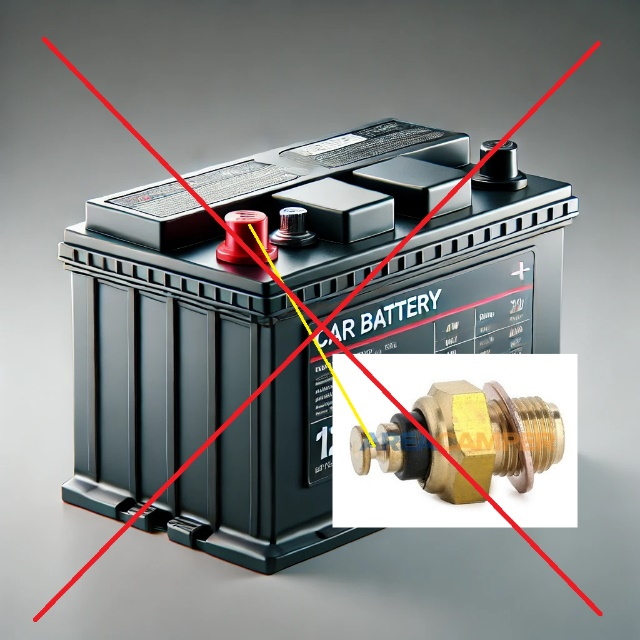
\includegraphics[width=\linewidth]{digifiz_manual/image002.jpg}
        \caption{Avertissement fourni avec le faisceau de capteurs contre toute tension externe.}
    \end{subfigure}
    \caption{Plaques de sécurité livrées avec le kit de câblage.}
\end{figure}

\chapter{Introduction}\label{ch:introduction}

Ce manuel d'exploitation couvre les blocs instruments numériques \ReplicaGenOne{} et \ReplicaNextLong{} destinés aux Volkswagen Golf~II, Jetta~II et Scirocco~II.
Il résume les variantes matérielles, décrit leurs fonctions et explique comment installer, configurer, utiliser, stocker et entretenir les tableaux de bord.
Les recommandations s'adressent aux propriétaires de véhicules, aux électriciens automobiles et aux ateliers qui rétrofitent le produit.

Les chapitres suivants présentent le schéma d'identification du produit, les brochages des connecteurs, les conditions de fonctionnement ainsi que des procédures détaillées d'installation et de configuration.
Des sections de maintenance et de dépannage pour les deux générations de Replica sont également incluses afin que le bloc compteur puisse être entretenu sans la documentation d'usine.

\begin{figure}[htbp]
    \centering
    \begin{subfigure}{0.48\textwidth}
        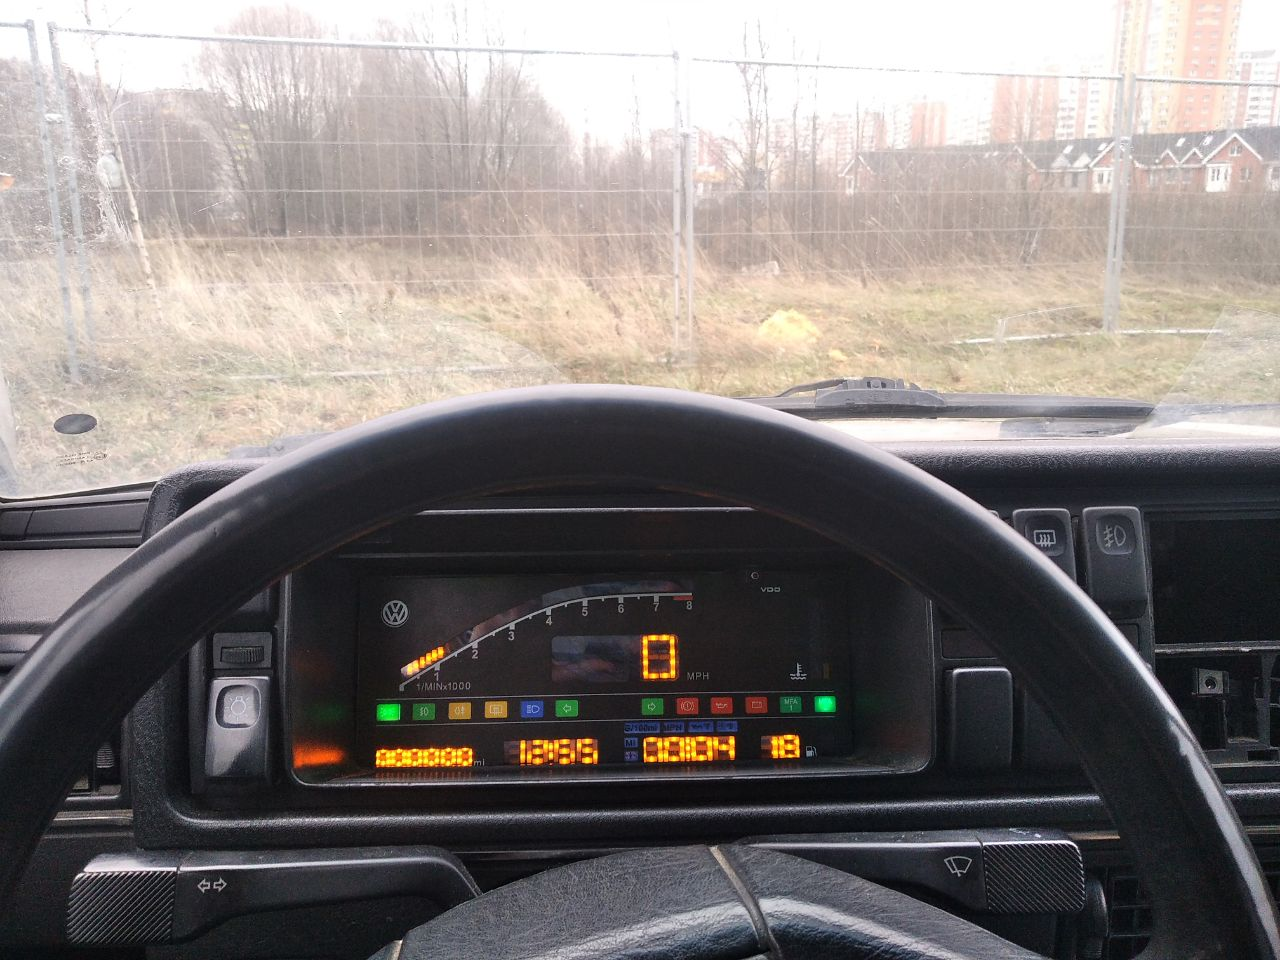
\includegraphics[width=\linewidth]{digifiz_manual/image004.jpg}
        \caption{Ensemble de livraison pour la configuration GART~8--MGF.}
    \end{subfigure}\hfill
    \begin{subfigure}{0.48\textwidth}
        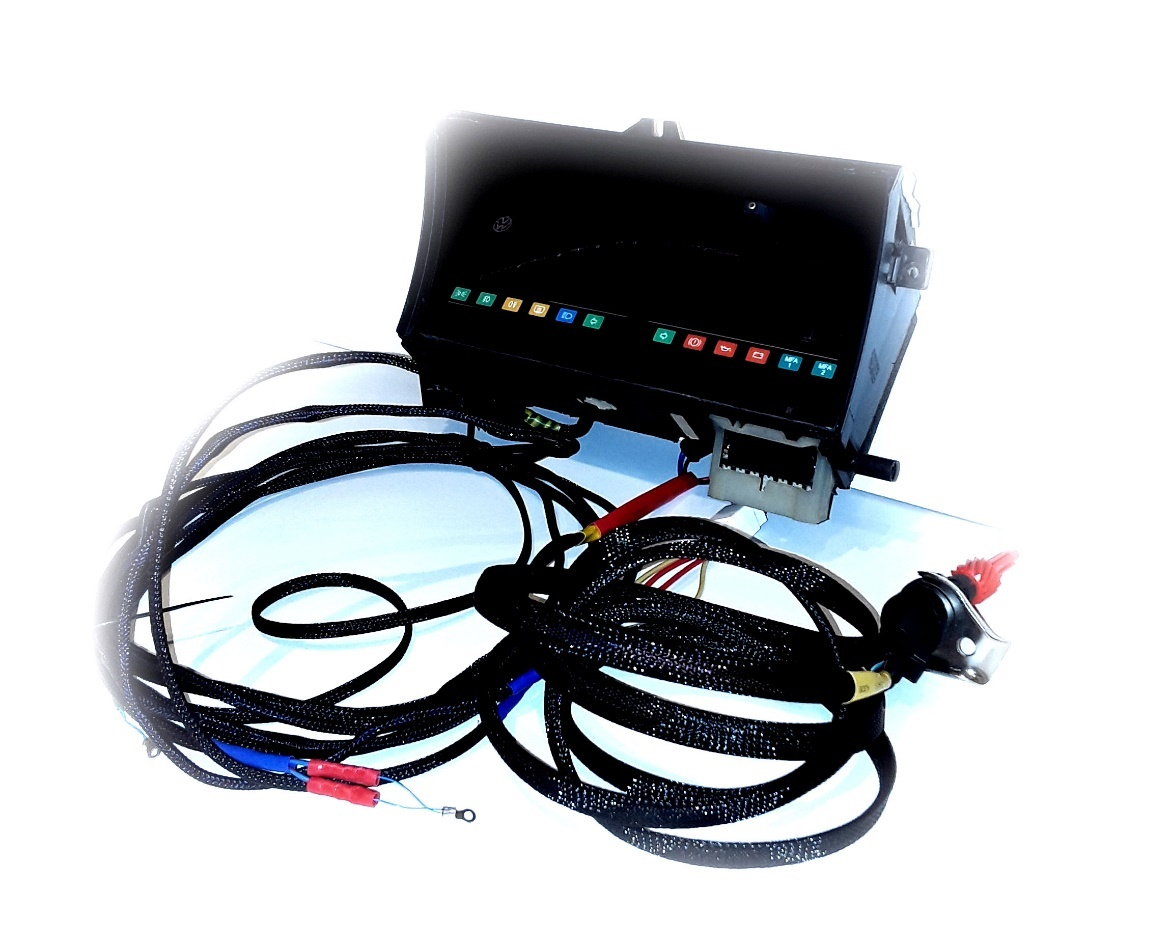
\includegraphics[width=\linewidth]{digifiz_manual/image005.jpg}
        \caption{Contenu typique d'un colis GART.}
    \end{subfigure}
    \begin{subfigure}{0.48\textwidth}
        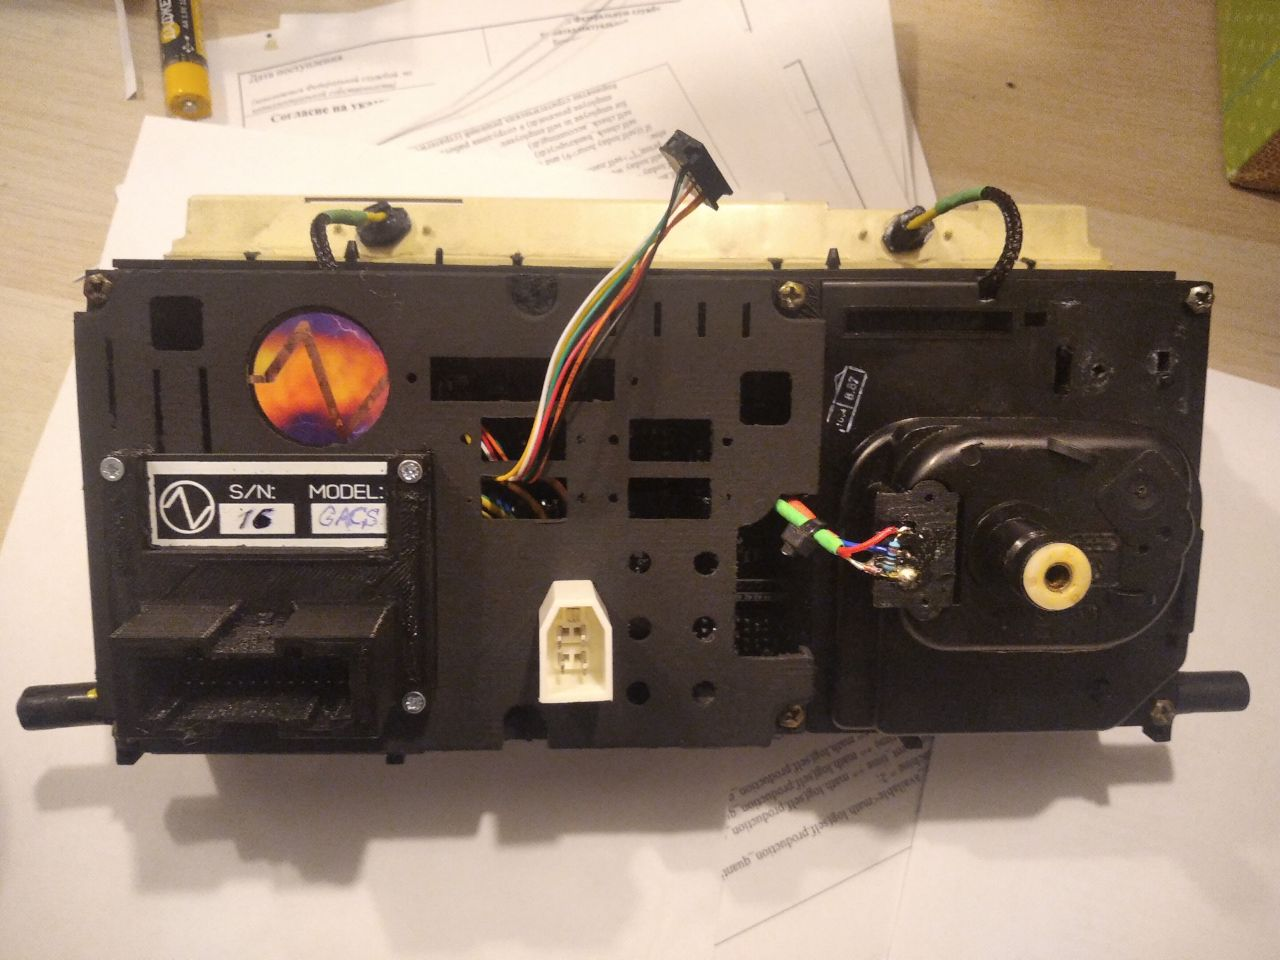
\includegraphics[width=\linewidth]{digifiz_manual/image006.jpg}
        \caption{Vue arrière de l'ensemble GACS à connecteur unique.}
    \end{subfigure}\hfill
    \begin{subfigure}{0.48\textwidth}
        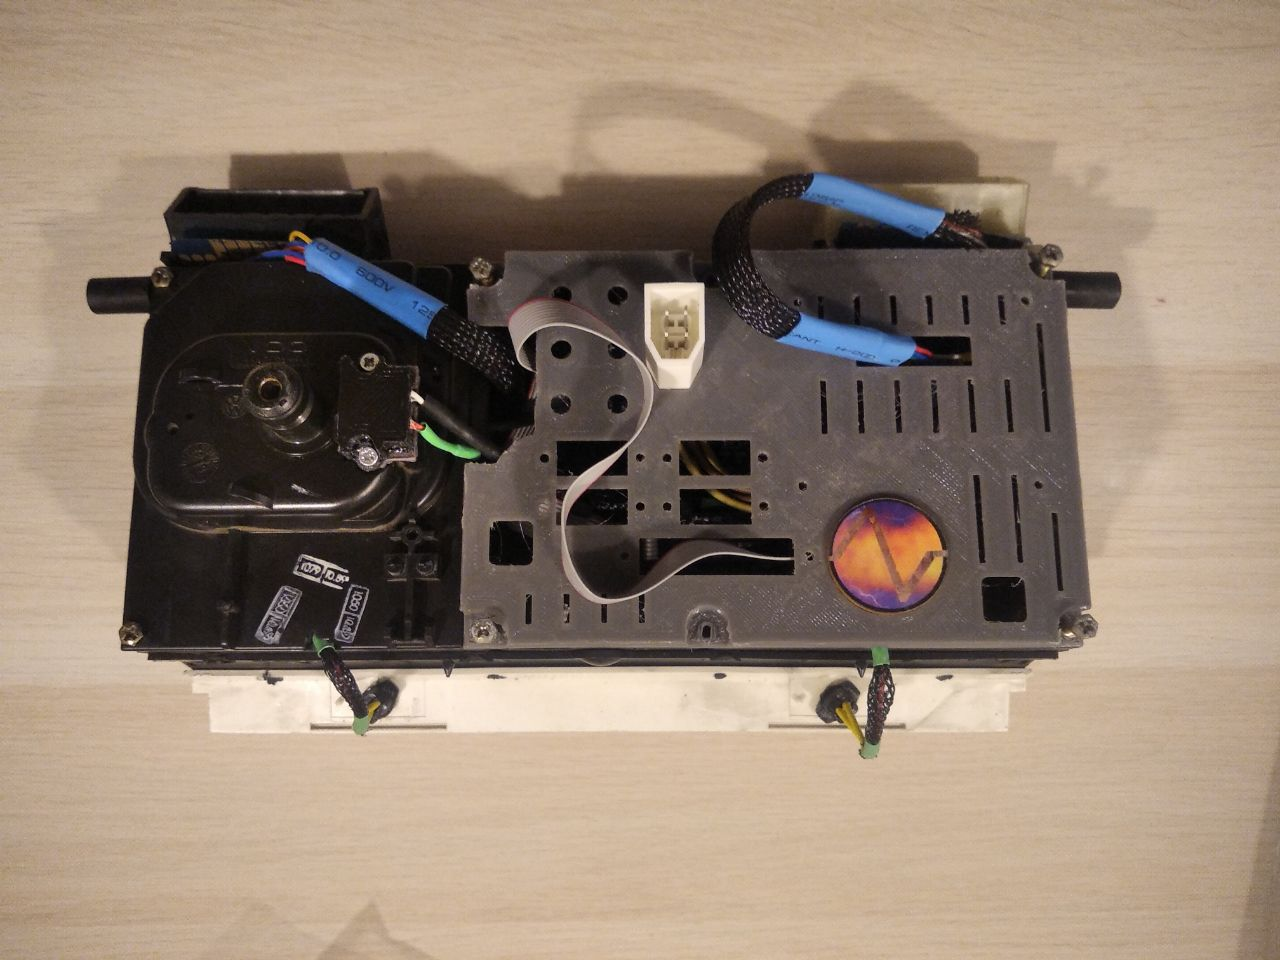
\includegraphics[width=\linewidth]{digifiz_manual/image007.jpg}
        \caption{Vue arrière de l'ensemble GACT à double connecteur.}
    \end{subfigure}
    \caption{Tableaux de bord \ReplicaGenOne{} et \ReplicaNextLong{} représentatifs fournis avec ce manuel.}
\end{figure}

Chaque variante est livrée avec les composants nécessaires à la chaîne cinématique visée, aux unités de mesure et au style de faisceau.
Les chapitres suivants déchiffrent les marquages des variantes et fournissent les tableaux de connecteurs afin que le bloc puisse être intégré en toute sécurité.

\chapter{Description et fonctionnement du produit}\label{ch:description}

\section{Objet}
Les tableaux de bord \ReplicaGenOne{} et \ReplicaNextLong{} remplacent les combinés Volkswagen d'origine tout en étendant leurs fonctionnalités.
Ils fournissent des indications numériques pour la vitesse, le régime moteur, la température du liquide de refroidissement, le niveau de carburant et les calculs auxiliaires de l'ordinateur de bord MFA, et prennent en charge aussi bien les capteurs de vitesse mécaniques qu'électroniques.
Les unités \ReplicaGenOneShort{} intègrent un contrôleur Bluetooth, tandis que \ReplicaNextShort{} ajoute des modules de configuration Wi-Fi et des unités d'extension optionnelles.

\section{Identification des modèles}
Chaque bloc compteur est marqué par un code de quatre lettres qui décrit la chaîne cinématique, le type d'assemblage, l'interface de capteur de vitesse et la génération de faisceau.
Des chiffres optionnels précisent l'échelle supportée par le compte-tours, et un suffixe supplémentaire de trois lettres indique les unités d'export.

\subsection{Désignation en quatre lettres}
\begin{description}
    \item[Position~1] \textbf{G} pour les moteurs essence ou \textbf{D} pour les moteurs diesel.
    \item[Position~2] \textbf{A} pour les unités assemblées en usine ou \textbf{M} pour les kits en auto-assemblage.
    \item[Position~3] \textbf{C} pour un capteur de vitesse mécanique à câble ou \textbf{R} pour un capteur de vitesse électronique.
    \item[Position~4] \textbf{T} pour le faisceau avant restylage (CE~1) ou \textbf{S} pour le faisceau restylé (CE~2).
\end{description}
Un chiffre final indique le régime moteur maximal affiché en milliers de tr/min (par exemple, « 8 » sur un bloc GACT8 correspond à une échelle 8000~tr/min).

\subsection{Suffixe d'unités}
Les variantes destinées à l'export peuvent ajouter un suffixe de trois lettres tiré de l'ensemble \texttt{MGFK}~:
\begin{description}
    \item[M] miles par heure,
    \item[G] gallons,
    \item[F] Fahrenheit,
    \item[K] Kelvin.
\end{description}
Par exemple, un tableau de bord \texttt{GART8-MGF} est une unité essence, assemblée en usine, pour capteur de vitesse électronique, faisceau CE~2, avec un compte-tours 8000~tr/min et des unités impériales.

\section{Gamme de modèles}
{\scriptsize
\begin{tblr}{
    colspec={Q[l,2.2cm] X[l]},
    hlines
}
\textbf{Modèle} & \textbf{Description} \\
GACT & Essence, entièrement assemblé, capteur de vitesse à câble, deux connecteurs, échelle 7000~tr/min. \\
GART & Essence, entièrement assemblé, capteur de vitesse électronique déporté, deux connecteurs, échelle 7000~tr/min. \\
GAC & Essence, entièrement assemblé, capteur de vitesse à câble, connecteur unique, échelle 7000~tr/min. \\
GARS & Essence, entièrement assemblé, capteur de vitesse électronique déporté, connecteur unique, échelle 7000~tr/min. \\
GACT8 & Essence, entièrement assemblé, capteur de vitesse à câble, deux connecteurs, échelle 8000~tr/min. \\
GART8 & Essence, entièrement assemblé, capteur de vitesse électronique déporté, deux connecteurs, échelle 8000~tr/min. \\
GACS8 & Essence, entièrement assemblé, capteur de vitesse à câble, connecteur unique, échelle 8000~tr/min. \\
GARS8 & Essence, entièrement assemblé, capteur de vitesse électronique déporté, connecteur unique, échelle 8000~tr/min. \\
DACT & Diesel, entièrement assemblé, capteur de vitesse à câble, deux connecteurs, échelle 6000~tr/min. \\
DART & Diesel, entièrement assemblé, capteur de vitesse électronique déporté, deux connecteurs, échelle 6000~tr/min. \\
DACS & Diesel, entièrement assemblé, capteur de vitesse à câble, connecteur unique, échelle 6000~tr/min. \\
DARS & Diesel, entièrement assemblé, capteur de vitesse électronique déporté, connecteur unique, échelle 6000~tr/min. \\
MT & Kit en auto-assemblage avec deux connecteurs. \\
M.S. & Kit en auto-assemblage avec un connecteur unique. \\
NEXT-GART & \ReplicaNextLong{}, échelle 8000~tr/min, deux connecteurs, capteur de vitesse électronique. \\
NEXT-GARS & \ReplicaNextLong{}, échelle 8000~tr/min, connecteur unique, capteur de vitesse électronique. \\
NEXT-MT & Kit \ReplicaNextLong{} en auto-assemblage avec deux connecteurs. \\
NEXT-MS & Kit \ReplicaNextLong{} en auto-assemblage avec un connecteur unique. \\
\end{tblr}}

\section{Brochage des connecteurs}
\subsection{Blocs à deux connecteurs}
\begin{figure}[htbp]
    \centering
    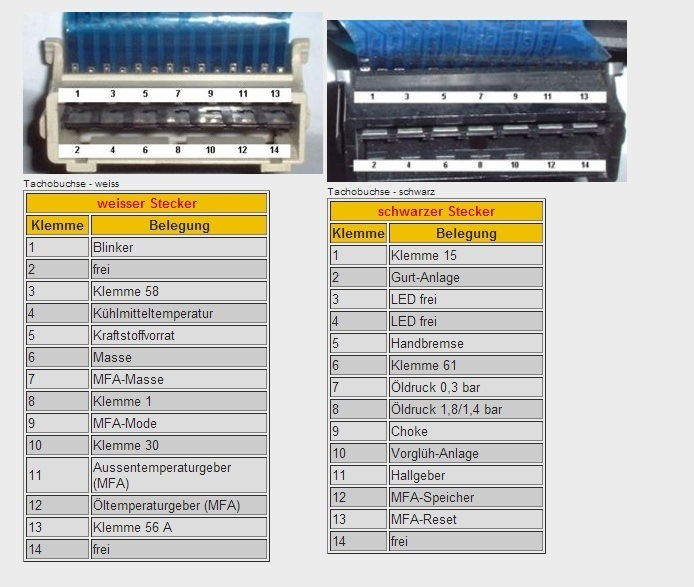
\includegraphics[width=0.72\textwidth]{digifiz_manual/image008.jpg}
    \caption{Disposition des connecteurs sur les tableaux \ReplicaGenOne{} à deux fiches.}
\end{figure}

\noindent\textbf{Connecteur blanc}

{\scriptsize
\begin{tblr}{
    colspec={Q[l,1.4cm] X[l]},
    hlines
}
\textbf{Broche} & \textbf{Affectation} \\
1 & Sortie clignotant, reliée à la masse pour le témoin lumineux. \\
2 & Frei --- non connecté. \\
3 & Borne~58, alimentation positive du rétroéclairage. \\
4 & Entrée de sonde de température de liquide de refroidissement résistive. \\
5 & Entrée de sonde de niveau de carburant résistive. \\
6 & Retour de masse. \\
7 & Retour de masse supplémentaire. \\
8 & Signal régime moteur borne~1 (bobine, distributeur ou autre forme jusqu'à 12~V avec des pics possibles à 300~V). \\
9 & Ligne de mode MFA utilisée pour changer les fonctions MFA. \\
10 & Alimentation permanente UNR (inutilisée sur \ReplicaGenOneShort{}, alimentation principale sur \ReplicaNextShort{}). \\
11 & Fil « + » de température MFA pour la sonde extérieure (\ReplicaNextShort{}). \\
12 & Fil de sonde de température d'huile MFA (\ReplicaNextShort{} uniquement). \\
13 & Entrée du témoin plein phare KL~56a (+12~V actif). \\
\end{tblr}}

\noindent\textbf{Connecteur noir}

{\scriptsize
\begin{tblr}{
    colspec={Q[l,1.4cm] X[l]},
    hlines
}
\textbf{Broche} & \textbf{Affectation} \\
1 & Borne~15, +12~V commuté depuis le contacteur d'allumage. \\
2--4 & Non connecté. \\
5 & Entrée du témoin de frein à main (actif à l'état bas). \\
6 & Pilotage de témoin d'alternateur KL~61 avec résistance d'excitation de 120~\ensuremath{\Omega}. \\
7 & Contact de pression d'huile 0,3~bar. \\
8 & Contact de pression d'huile 1,8~bar. \\
9 & Non utilisé. \\
10 & Entrée du témoin de préchauffage (+12~V actif, diesel uniquement). \\
11 & Entrée capteur Hall pour capteurs de vitesse optionnels. \\
12 & Ligne de sélection de bloc MFA. \\
13 & Ligne de remise à zéro MFA. \\
\end{tblr}}

\subsection{Blocs à connecteur unique}
Les tableaux à connecteur unique utilisent le câblage illustré à l'\autoref{fig:single-connector}.
Le faisceau reproduit les mêmes signaux que les variantes à deux connecteurs, mais les regroupe dans une seule fiche.

\begin{figure}[htbp]
    \centering
    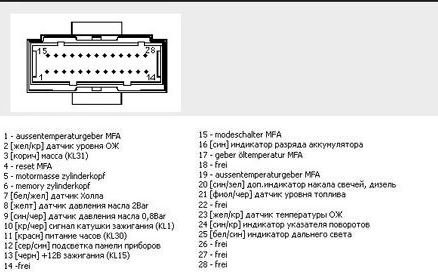
\includegraphics[width=0.65\textwidth]{digifiz_manual/image009.png}
    \caption{Disposition du connecteur unique utilisé sur les tableaux Replica compacts.}
    \label{fig:single-connector}
\end{figure}

\subsection{Faisceau prospectif Scirocco/Passat}
Le faisceau prospectif Scirocco/Passat utilise deux fiches.
Leurs fonctions sont résumées ci-dessous.

\noindent\textbf{Fiche 5~broches}
{\scriptsize
\begin{tblr}{
    colspec={Q[l,2.6cm] X[l]},
    hlines
}
\textbf{Broche} & \textbf{Affectation} \\
1~(D3) & Contact d'indication de gamme « D » de la boîte automatique. Met le témoin de conduite à la masse lorsque le sélecteur est en position~D. \\
2~(D2) & Contact d'indication de deuxième gamme de la boîte automatique. Met le témoin « 2 » à la masse lorsque le sélecteur est en position~2. \\
3~(D1) & Contact d'indication de première gamme de la boîte automatique. Met le témoin « 1 » à la masse lorsque le sélecteur est en position~1. \\
4~(SA) & Alimentation commune de l'affichage de sélecteur automatique (\emph{Schaltanzeige}); fournit le +12~V aux voyants de gamme. \\
5~(SPERRE) & Contact d'interverrouillage de démarrage provenant du sélecteur. Fermé en position parking ou point mort pour autoriser le démarrage. \\
\end{tblr}}

\noindent\textbf{Fiche 14~broches}
{\scriptsize
\begin{tblr}{
    colspec={Q[l,2.6cm] X[l]},
    hlines
}
\textbf{Broche} & \textbf{Affectation} \\
1~(KL~58) & Alimentation d'éclairage pour le rétroéclairage du panneau. \\
2~(MASS) & Retour de masse châssis. \\
3~(TANK) & Entrée jauge de carburant. \\
4~(TEMP) & Entrée sonde de température de liquide de refroidissement. \\
5~(KL~1) & Signal de régime moteur (borne~1). \\
6~(UHR) & +12~V permanent pour l'horloge et la sauvegarde mémoire. \\
7~(FERNL) & Entrée témoin plein phare. \\
8~(reserved) & Non connecté. \\
9~(OEL~1.8) & Contact de pression d'huile haute, 1,8~bar. \\
10~(CAT~VORGL(-)) & Entrée témoin de préchauffage catalyseur/diesel (actif bas). \\
11~(OEL~0.3) & Contact de pression d'huile basse, 0,3~bar. \\
12~(KL~61) & Témoin d'alternateur et alimentation d'excitation. \\
13~(KL~49a) & Alimentation combinée du témoin de clignotants. \\
14~(KL~15) & Alimentation +12~V commutée par l'allumage. \\
\end{tblr}}

\subsection{Correspondance des connecteurs Mk1}
Les véhicules Volkswagen Mk1 utilisent les affectations suivantes~:
\begin{enumerate}
    \item Alimentation d'éclairage et de feux de croisement.
    \item Masse MASSE~31.
    \item Émetteur de niveau de carburant TANK.
    \item Sonde de température TEMP.
    \item Signal de compte-tours KL~1.
    \item +12~V permanent UHR.
    \item Signal plein phare KL~56.
    \item Contact de pression d'huile (HAUTE) 1,8~bar.
    \item Contact de pression d'huile (BASSE) 0,3~bar.
    \item Témoin de préchauffage diesel.
    \item Entrée starter (non utilisée).
    \item Lampe génératrice KL~61.
    \item Entrée clignotant (gauche/droite combinés).
    \item Alimentation d'allumage KL~15.
\end{enumerate}
\begin{figure}[htbp]
    \centering
    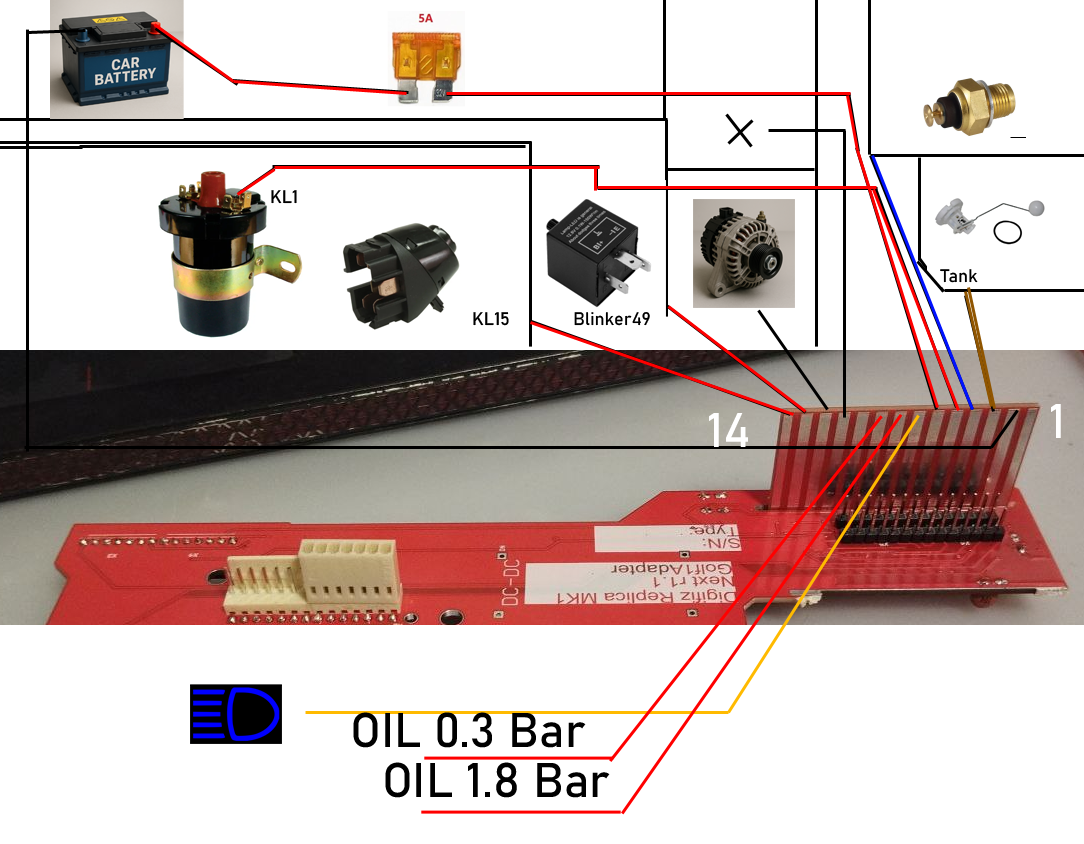
\includegraphics[width=0.75\textwidth]{digifiz_manual/image010.png}
    \caption{Schéma de connexion du faisceau pour les installations Mk1.}
\end{figure}

\subsection{Connecteur de service sur la carte}
Le troisième connecteur sur la carte reproduit les connecteurs du tableau, avec des broches numérotées de droite à gauche sur les unités \ReplicaGenOneShort{} et \ReplicaNextShort{}.
Il fournit une interface de service avec les affectations listées dans l'\autoref{tab:service-connector}.

\begin{table}[htbp]
    \centering
    \caption{Affectations des broches du connecteur de service.}
    \label{tab:service-connector}
    {\scriptsize
    \begin{tblr}{
        colspec={Q[l,1.9cm] X[l]},
        hlines,
    }
        \textbf{Position} & \textbf{Affectation} \\
        1 & Sortie témoin. \\
        2 & Entrée capteur de vitesse (SPM\_M). \\
        3 & Masse véhicule. \\
        4 & Sortie témoin. \\
        5 & Entrée optocoupleur clignotant gauche. \\
        6 & Entrée optocoupleur clignotant droit. \\
        7 & +12~V contact. \\
        8 & Entrée spécifique diesel. \\
        9 & Entrée témoin (positive). \\
        10 & Entrée régime alternative (inutilisée, \ReplicaNextShort{} uniquement). \\
        11 & \ReplicaGenOneShort{} : sortie témoin (normalement déconnectée) ; \ReplicaNextShort{} : entrée frein (active bas). \\
        12 & Réservé. \\
        13 & Entrée voyant moteur. \\
        14 & Aucun contact. \\
    \end{tblr}}
\end{table}

\subsection{Connecteurs d'extension auxiliaires}
Trois barrettes supplémentaires à quatre broches sont montées sur la carte principale pour faciliter les évolutions de faisceau et les opérations de service~:
\begin{itemize}
    \item \textbf{Signaux analogiques d'extension~:} offre un accès dédié pour ajouter des entrées analogiques lors de l'intégration de capteurs personnalisés.
    \item \textbf{Miroir MFA~:} duplique le connecteur \textsc{MFA} standard pour permettre un piquage parallèle des signaux de l'ordinateur de bord.
    \item \textbf{Doublons analogiques~:} répète les entrées température d'huile, température ambiante et témoin de frein afin de les router vers des modules de journalisation ou de surveillance externes.
\end{itemize}
Les trois utilisent le connecteur femelle \mbox{KF2510-4p}, non fourni avec le kit tableau de bord et à se procurer séparément si nécessaire.

\begin{figure}[htbp]
    \centering
    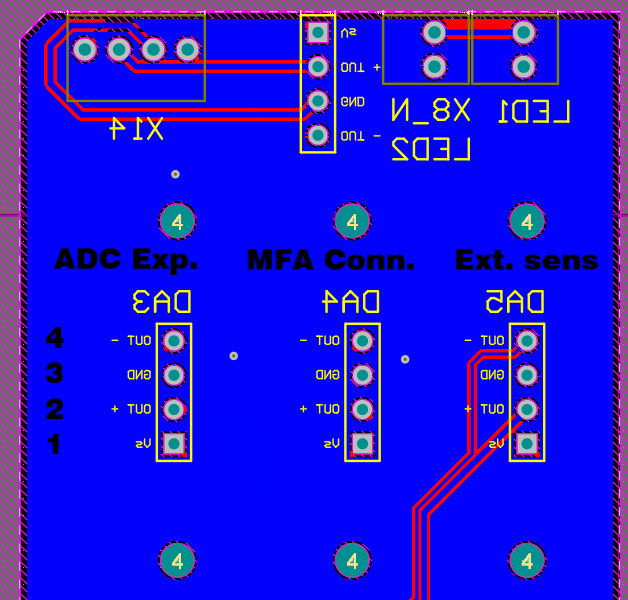
\includegraphics[width=0.6\textwidth]{digifiz_manual/ext_conn.png}
    \caption{Disposition des connecteurs auxiliaires sur la carte principale.}
\end{figure}

\begin{table}[htbp]
    \centering
    {\small
    \begin{tblr}{
        colspec={Q[l,2.3cm] Q[c,1.3cm] X[l]},
        hlines,
        row{1} = {font=\bfseries}
    }
    Connecteur & Broche & Affectation \\
    Connecteur~I & 4 & Entrée analogique auxiliaire~1 \\
    Connecteur~I & 3 & Masse (GND) \\
    Connecteur~I & 2 & Entrée analogique auxiliaire~2 \\
    Connecteur~I & 1 & VCC (3V3, non protégée\textbf{!!!}) \\
    Connecteur~II & 4 & Remise à zéro MFA \\
    Connecteur~II & 3 & Masse (GND) \\
    Connecteur~II & 2 & Bloc mémoire MFA \\
    Connecteur~II & 1 & Mode MFA \\
    Connecteur~III & 4 & Sortie sonde de température d'huile \\
    Connecteur~III & 3 & Masse (GND) \\
    Connecteur~III & 2 & Sortie sonde de température extérieure \\
    Connecteur~III & 1 & Témoin de frein \\
    \end{tblr}}
    \caption{Affectations des connecteurs d'extension auxiliaires.}
\end{table}

\section{Logiciel embarqué et contenu}
Le micrologiciel du tableau de bord est publié à l'adresse suivante~:
\displayurl{https://github.com/Sgw32/DigifizReplica}
Deux ensembles de livraison sont disponibles~:
\begin{itemize}
    \item \textbf{\ReplicaGenOne{}~:} tableau de bord, faisceau de température d'air et d'huile, programmateur USBasp et, pour les capteurs déportés, faisceau de capteur de vitesse.
    \item \textbf{\ReplicaNextLong{}~:} tableau de bord et faisceau pour capteur de vitesse électronique.
\end{itemize}

\chapter{Principe de fonctionnement} \label{ch:operating-principle}

Les tableaux \ReplicaGenOne{} réutilisent le boîtier Volkswagen d'origine, les connecteurs CE~1 ou CE~2 du constructeur et, selon la configuration, soit le câble de compteur de vitesse mécanique soit un capteur de vitesse électronique.
Les cartes principales \ReplicaGenOneShort{} reposent sur un circuit imprimé en fibre de verre peuplé de composants discrets pilotés par un microcontrôleur ATmega~2560 et des pilotes d'afficheurs MAX~7219.

\ReplicaNextLong{} s'appuie sur un système sur puce ESP32-S3 et introduit un boîtier nouvellement fabriqué en impression SLA, une façade et un capot repensés ainsi qu'une carte adaptatrice de connecteur.
L'afficheur \ReplicaNextShort{} est rétroéclairé par des LED adressables WS2812 montées derrière la façade, et le faisceau associé inclut d'office le capteur de vitesse électronique.

Les deux générations partagent la même disposition d'affichage et les mêmes pages MFA, ce qui garantit des procédures d'installation et une utilisation quotidienne familières d'une révision matérielle à l'autre.

\chapter{Caractéristiques techniques}\label{ch:technical-specs}

Le tableau \ReplicaGenOne{} ne consomme aucun courant de veille lorsqu'il est hors tension.
\ReplicaNextShort{} tire environ 13~mA du +12~V contact coupé, point à prendre en compte lors d'un stationnement prolongé du véhicule.
Les deux générations fonctionnent de manière fiable sur le réseau électrique automobile entre 9~V et 16~V\,CC.

\section{Capacités de mesure}
\begin{itemize}
    \item \textbf{Vitesse véhicule~:} mesurée via le câble d'origine ou un capteur de vitesse électronique. L'erreur systématique est de 10~km/h, l'erreur relative de 3~km/h, et l'affichage se sature à 999~km/h (ou mph pour les unités impériales).
    \item \textbf{Régime moteur~:} dérivé du signal d'allumage au travers d'un étage optocoupleur avec réseau RC 430~nF/1,2~k\ensuremath{\Omega} et diode de limitation. Les erreurs absolue et relative restent dans une plage de 200~tr/min.
    \item \textbf{Niveau de carburant~:} lu sur la jauge résistive du réservoir avec une incertitude d'environ 10~litres.
    \item \textbf{Température de liquide de refroidissement~:} indiquée qualitativement via la thermistance d'origine connectée par le faisceau ; aucune valeur numérique n'est affichée.
    \item \textbf{Horodatage~:} maintien de l'heure à une minute près.
    \item \textbf{Voyants~:} clignotants, plein phare, alertes de pression d'huile, état de l'alternateur, frein à main, dégivrage de lunette arrière ou bougies de préchauffage diesel, et antibrouillards avant/arrière.
\end{itemize}

\chapter{Conditions d'utilisation et consignes de sécurité}\label{ch:safety}

\section{Limites environnementales}
\begin{itemize}
    \item Le combiné fonctionne entre \(-40\,^{\circ}\mathrm{C}\) et \(+70\,^{\circ}\mathrm{C}\) pour une humidité relative pouvant atteindre 95~\%.
    \item Le tableau de bord peut rester installé dans le véhicule toute l'année, y compris lors d'un stationnement prolongé.
\end{itemize}

\section{Consignes de sécurité}
\begin{enumerate}
    \item Le tableau Digifiz est un appareil assemblé et intégré par des passionnés. Respectez les règles générales de sécurité électrique lors des travaux.
    \item Le produit est destiné aux projets personnels des propriétaires de véhicules.
    \item Les indications ne sont ni certifiées ni vérifiées métrologiquement, bien qu'elles correspondent aux spécifications annoncées lors de la publication.
    \item N'utilisez le tableau de bord que si vous acceptez la responsabilité de l'installation et de la sécurité routière.
    \item Si les données affichées vous semblent douteuses, vérifiez-les à l'aide des instruments standard du véhicule ou d'appareils de mesure externes.
    \item N'utilisez pas les sorties du combiné pour des systèmes de contrôle automatique du véhicule.
    \item Les auteurs déclinent toute responsabilité quant aux conséquences liées à l'installation ou à l'utilisation du tableau, y compris les amendes ou accidents. Les dysfonctionnements signalés durant la période de garantie (un an pour les installations réalisées avec les auteurs et deux semaines pour les installations autonomes) seront réparés.
    \item Les performances fonctionnelles décrites au \Cref{ch:technical-specs} sont garanties pendant un an dans le cadre d'une installation supervisée et durant deux semaines après une installation indépendante.
\end{enumerate}

\chapter{Préparation du travail et ordre des opérations}\label{ch:preparation}

\section{Préparation du véhicule}
Suivez la séquence ci-dessous pour remplacer le combiné d'origine par un tableau Digifiz~:
\begin{enumerate}
    \item Retirez les garnitures plastiques recouvrant les pédales et la partie inférieure du tableau de bord pour mettre à nu le bloc instruments d'usine.
    \item Débranchez la batterie du véhicule.
    \item Déconnectez le faisceau du combiné d'origine.
    \item Désaccouplez le câble de compteur mécanique, s'il est présent.
    \item Dévissez le combiné de ses supports et retirez-le délicatement du véhicule.
    \item Faites cheminer les faisceaux de température et de capteur de vitesse fournis selon les besoins.
    \item Installez le tableau Digifiz dans les glissières de support et fixez-le avec les vis.
    \item Pour \ReplicaNextLong{}, installez les capteurs Volkswagen MFA (ou équivalents) et amenez leurs fils vers les connecteurs CE~1/CE~2.
    \item Sur les modèles \texttt{GACS}/\texttt{GARS}/\texttt{DARS}/\texttt{DACS}, raccordez manuellement les fils étiquetés \texttt{MFA\_MODE}, \texttt{MFA\_RESET}, \texttt{MFA\_BLOCK} et frein à main si le faisceau véhicule ne possède pas ces contacts. La seconde génération \ReplicaNextShort{} relie ces signaux en interne par défaut.
    \item Branchez les faisceaux sur le tableau.
    \item Montez le capteur de vitesse électronique ou reconnectez le câble mécanique.
    \item Reposez les garnitures du tableau de bord et le cache-pédales dans l'ordre inverse.
\end{enumerate}

\section{Utilisation du tableau}
\begin{itemize}
    \item Le tableau s'alimente automatiquement avec le contact. L'interrupteur des feux de position commande le rétroéclairage.
    \item Au démarrage, toute l'échelle de vitesse s'allume pendant que les diagnostics internes stabilisent le modèle de régime ; l'affichage se fixe ensuite sur le ralenti courant.
    \item Dès que le véhicule se met en mouvement, le système indique les paramètres listés au \Cref{ch:technical-specs}.
\end{itemize}

\subsection{Fonctions MFA}
Six pages MFA sont disponibles~:
\begin{enumerate}
    \item Durée de fonctionnement journalière.
    \item Distance parcourue.
    \item Consommation de carburant (non implémentée sur la première révision Replica).
    \item Vitesse moyenne (affichée multipliée par dix).
    \item Température d'huile moteur (faisceau externe requis).
    \item Température ambiante (faisceau externe requis).
\end{enumerate}
Sur les tableaux \ReplicaGenOneShort{}, un point tactile capacitif derrière le logo VW fait défiler les pages ; \ReplicaNextShort{} utilise un commutateur de colonne externe. Les durées de contact se comportent ainsi~:
\begin{itemize}
    \item Appui court (\(<1\)~s)~: passe à la fonction MFA suivante.
    \item Appui moyen (1--3~s en l'absence de commutateur de colonne)~: change de bloc mémoire MFA ; la modification est indiquée à l'écran.
    \item Appui long (3--7~s)~: réinitialise la fonction MFA active (consommation, distance, durée et vitesse moyenne).
\end{itemize}

\subsection{Rétroéclairage et disposition des voyants}
Le tableau \ReplicaGenOneShort{} propose une molette de luminosité manuelle au-dessus de l'interrupteur des feux de stationnement ; \ReplicaNextShort{} s'appuie sur un réglage automatique piloté par photodiode. Des dérogations manuelles peuvent être configurées via les interfaces de maintenance décrites aux \Cref{ch:replica-setup,ch:replica-next-setup}.

La disposition de la barre horizontale de voyants et la légende à l'écran sont illustrées à l'\autoref{fig:indicator-layout}.

\begin{figure}[htbp]
    \centering
    \begin{subfigure}{0.48\textwidth}
        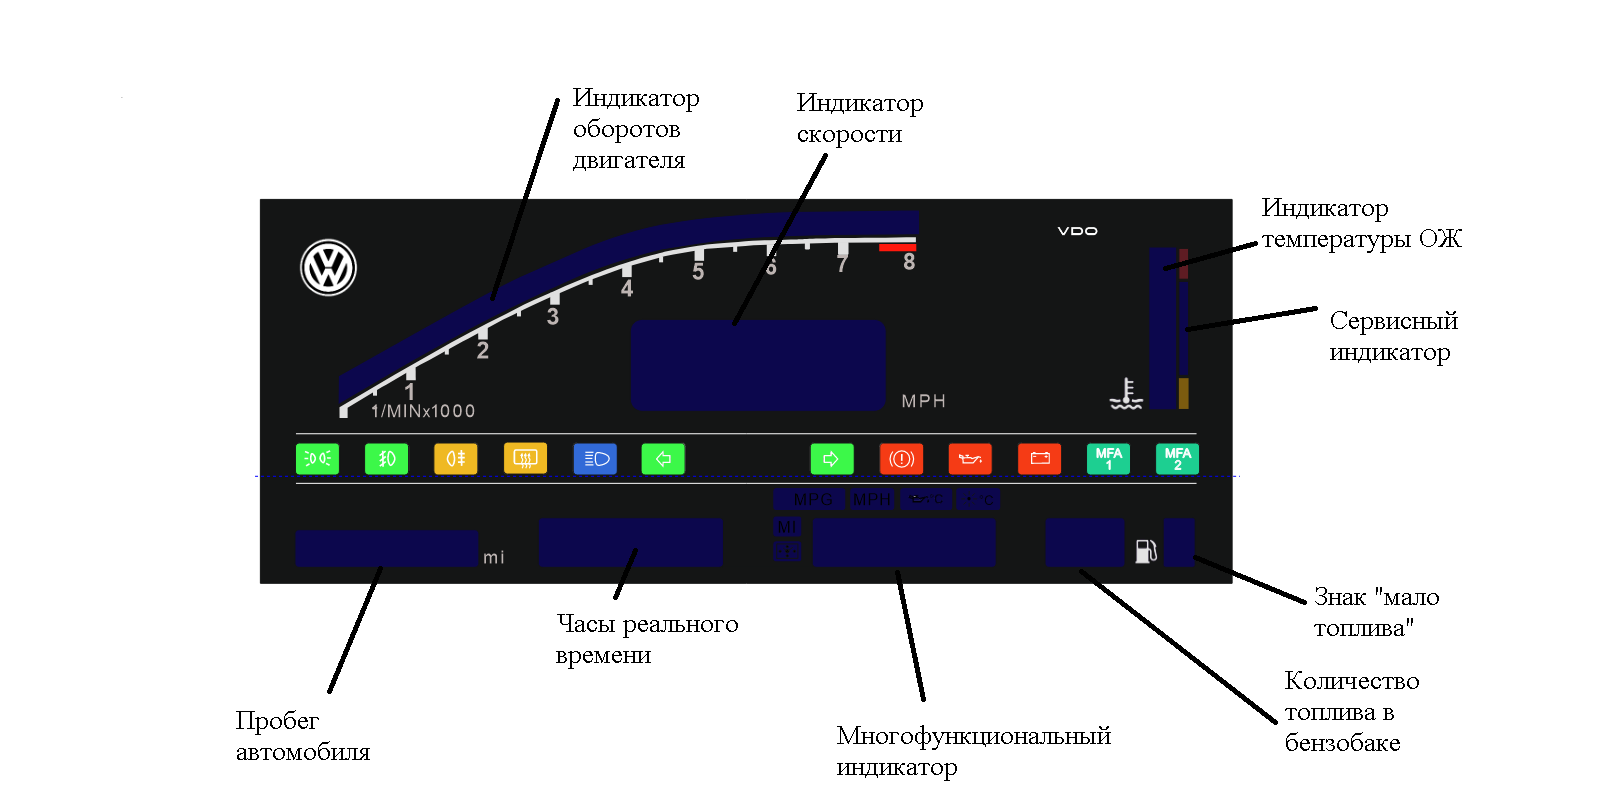
\includegraphics[width=\linewidth]{digifiz_manual/image017.png}
        \caption{Disposition des voyants affichée lors de l'auto-test.}
    \end{subfigure}\hfill
    \begin{subfigure}{0.48\textwidth}
        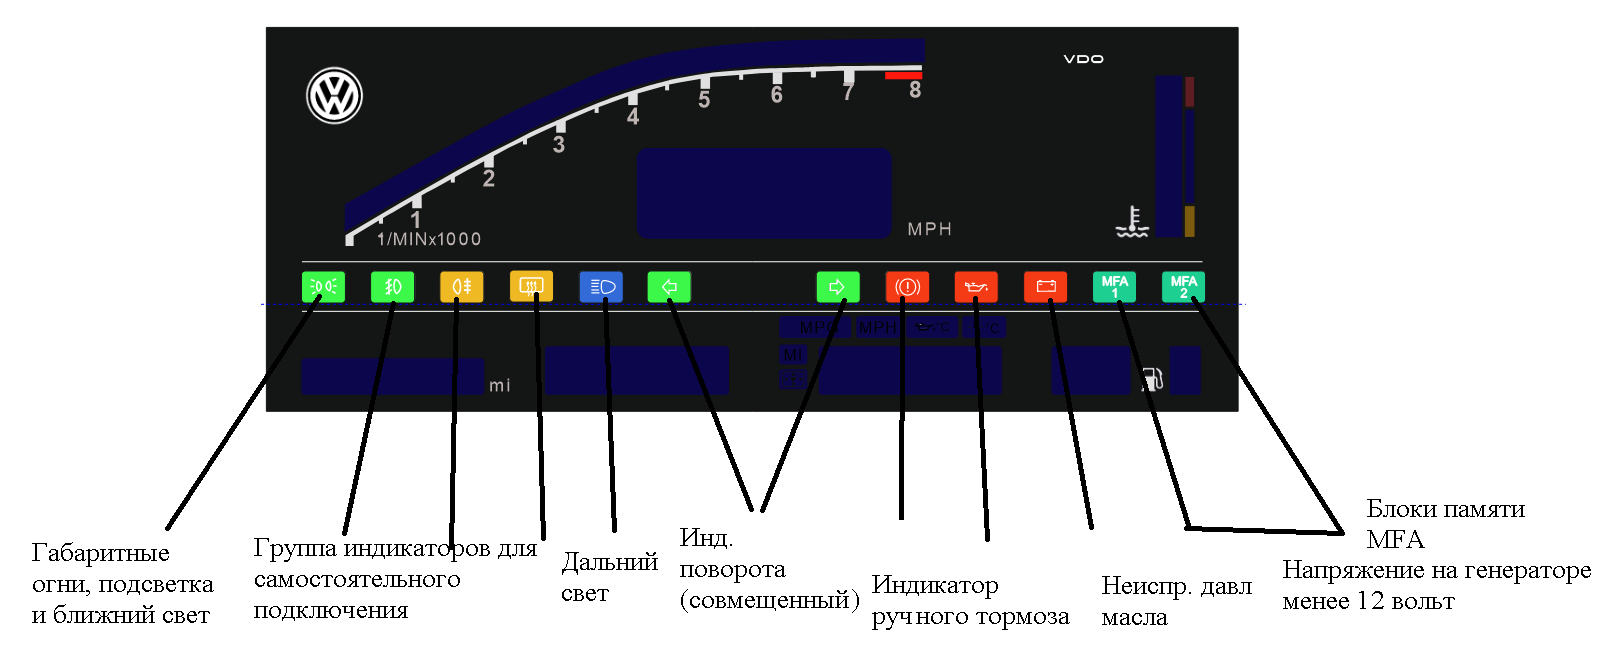
\includegraphics[width=\linewidth]{digifiz_manual/image018.png}
        \caption{Légende de la barre horizontale de voyants.}
    \end{subfigure}
    \caption{Schéma d'indication du combiné.}
    \label{fig:indicator-layout}
\end{figure}

\subsection{Interfaces de configuration}
\begin{itemize}
    \item Les unités \ReplicaGenOne{} classiques intègrent un module Bluetooth 2.0 (ou compatible BLE). Installez l'application \emph{Serial Bluetooth Terminal} depuis Google Play, associez-la au tableau et envoyez les commandes depuis la console. Les appareils Apple iOS ne peuvent pas se connecter à ce module.
    \item \ReplicaNextShort{} expose un point d'accès Wi-Fi embarqué et un portail de configuration décrits au \Cref{ch:replica-next-setup}. Désactivez les données mobiles pendant la connexion pour que le portail captif se charge correctement.
\end{itemize}
Les deux générations peuvent également être alimentées et configurées sur établi via l'interface de programmation USBasp.

\chapter{Configuration et maintenance de \ReplicaNextLong{}}\label{ch:replica-next-setup}

Cette section s'applique au tableau \ReplicaNextLong{} illustré à l'\autoref{fig:next-hardware}.

\begin{figure}[htbp]
    \centering
    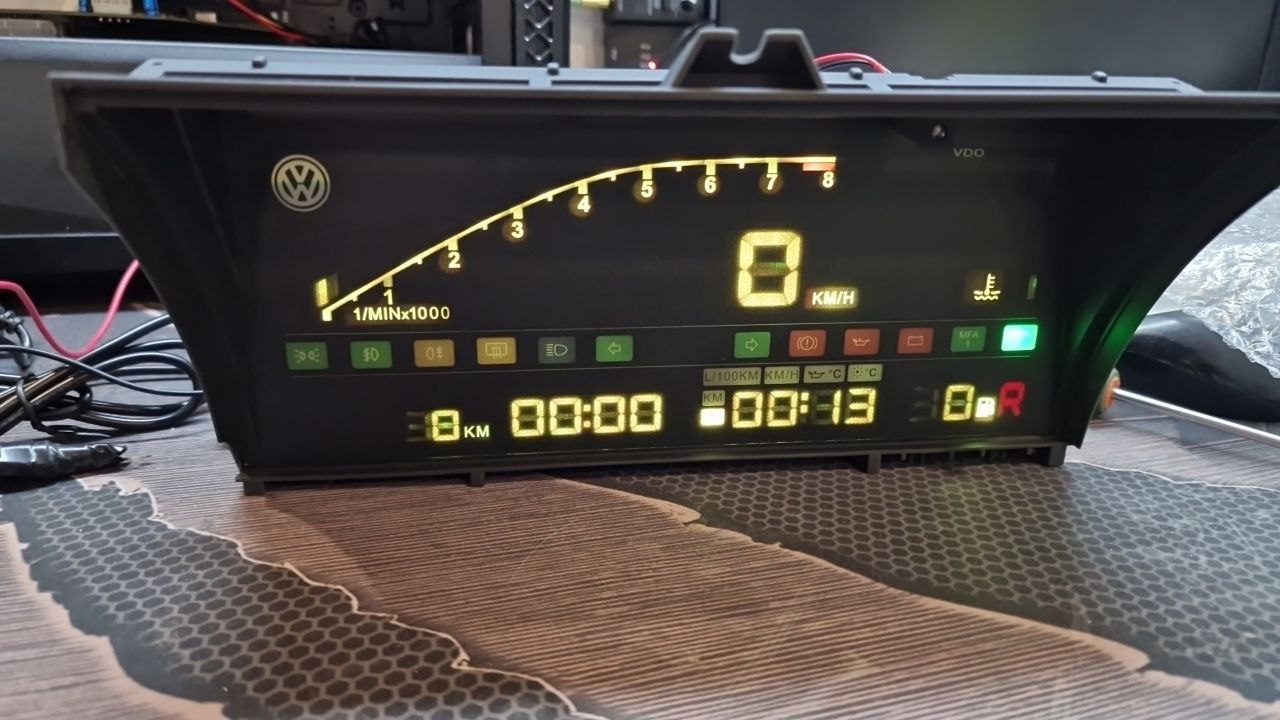
\includegraphics[width=0.6\textwidth]{digifiz_manual/image019.png}
    \caption{Assemblage du tableau \ReplicaNextLong{}.}
    \label{fig:next-hardware}
\end{figure}

\section{Manipulation du combiné}
\begin{itemize}
    \item La façade en polycarbonate imprimée aux UV doit être protégée des rayures et corps étrangers. Toute détérioration importante nécessite des pièces de rechange auprès de PHOL-LABS Kft et n'est pas couverte par la garantie.
    \item L'horloge temps réel se règle via le portail Wi-Fi. Elle se réinitialise dès que l'alimentation permanente est coupée.
\end{itemize}

\section{Portail de contrôle Wi-Fi}
La configuration, la collecte de données et la gestion du micrologiciel s'effectuent via l'application web embarquée.
\begin{itemize}
    \item Connectez-vous au point d'accès Wi-Fi du tableau. Désactivez les données mobiles et rejoignez \texttt{Digifiz\_AP} (mot de passe \texttt{87654321}); certaines révisions annoncent \texttt{PHOL-LABS2} avec le même mot de passe.
    \item L'adresse IP par défaut est \texttt{192.168.4.1}. Si le tableau est configuré pour rejoindre un autre réseau, analysez le sous-réseau à la recherche d'une adresse se terminant par \texttt{.32} à l'aide d'un utilitaire IP.
    \item Le portail comporte trois onglets~: \emph{WiFi}, \emph{Control} et \emph{About} (\autoref{fig:next-control-tabs}). L'onglet WiFi gère les paramètres réseau et les mises à jour de micrologiciel ; l'onglet Control ajuste les paramètres du tableau ; l'onglet About récapitule les informations sur les auteurs.
\end{itemize}

\begin{figure}[htbp]
    \centering
    \begin{subfigure}{0.48\textwidth}
        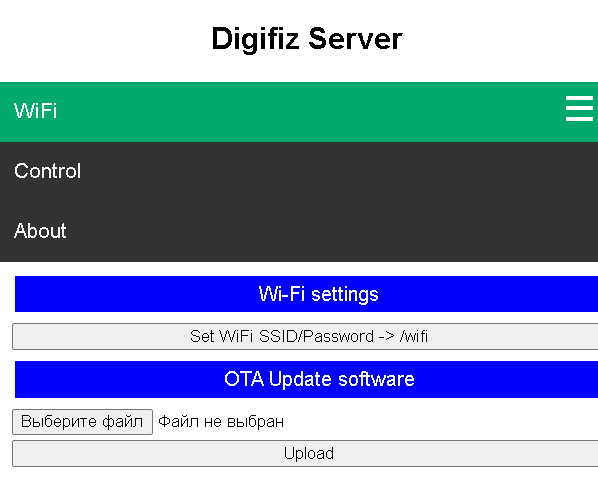
\includegraphics[width=\linewidth]{digifiz_manual/image020.png}
        \caption{Vue d'ensemble de l'onglet Control.}
    \end{subfigure}\hfill
    \begin{subfigure}{0.48\textwidth}
        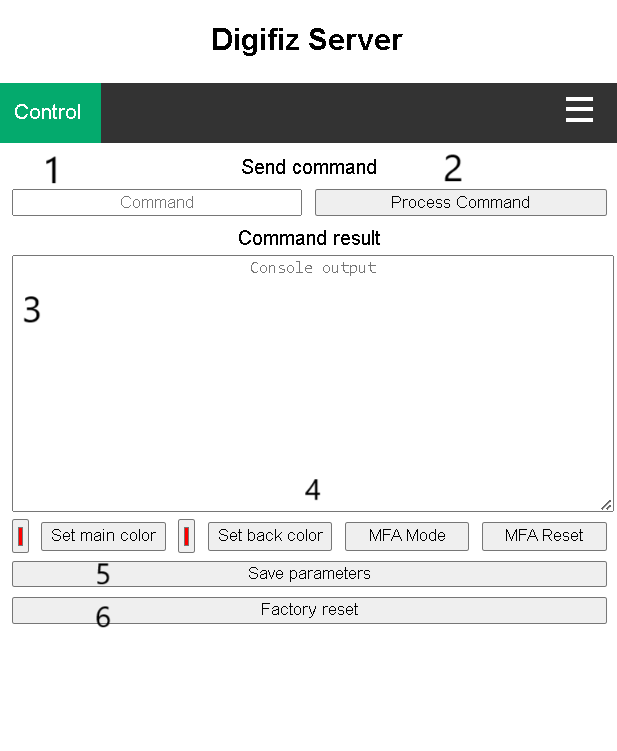
\includegraphics[width=\linewidth]{digifiz_manual/image021.png}
        \caption{Commandes numérotées et zones de saisie.}
    \end{subfigure}
    \caption{Interface Wi-Fi de \ReplicaNextShort{}.}
    \label{fig:next-control-tabs}
\end{figure}

\section{Saisie de commandes}
L'onglet \emph{Control} met à disposition une ligne de commande (1), un bouton \emph{Process} (2), une fenêtre de résultat (3), des réglages rapides (4), un bouton \emph{Save} (5) et un bouton \emph{Reset} (6).
Saisissez les commandes sous la forme de paires séparées par un espace \verb|<numéro> <valeur>| en utilisant uniquement des entiers ; la ponctuation et les guillemets sont inutiles.
L'\autoref{fig:next-command-example} illustre l'interface lors de la désactivation du réglage automatique de luminosité.

\begin{figure}[htbp]
    \centering
    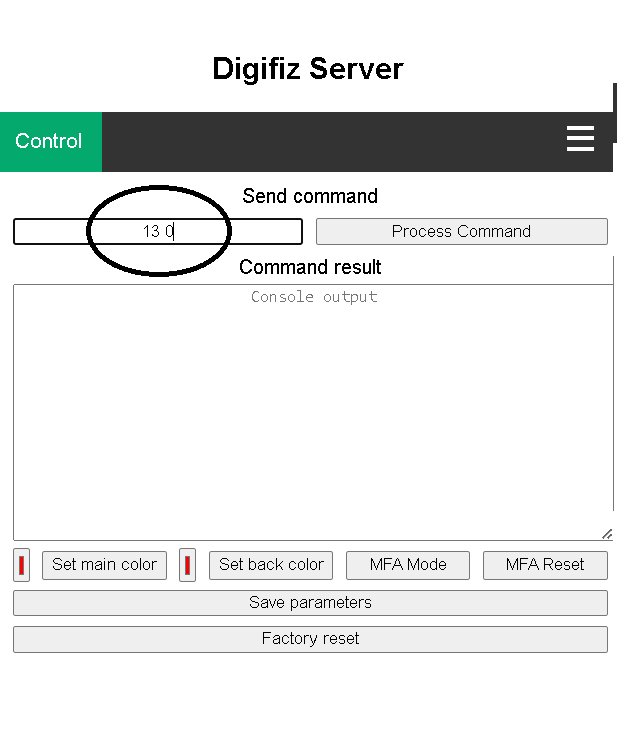
\includegraphics[width=0.55\textwidth]{digifiz_manual/image022.png}
    \caption{Exemple de commande désactivant la luminosité automatique.}
    \label{fig:next-command-example}
\end{figure}

\section{Référence de commandes}
\begin{table}[htbp]
    \centering
    \caption{Commandes principales de configuration \ReplicaNextShort{}.}
    \label{tbl:next-commands}
    {\scriptsize
    \begin{tblr}{
        colspec = {Q[c,0.14\linewidth] Q[l,0.36\linewidth] Q[l]},
        rowsep = 2pt,
    }
        \toprule
        \textbf{Commande} & \textbf{Nom} & \textbf{Description} \\
        \midrule
        22 (ou 0) & \paramname{PARAMETER\_RPMCOEFFICIENT} & Facteur d'étalonnage du régime (100--10000). \\
        1  & \paramname{PARAMETER\_SPEEDCOEFFICIENT} & Facteur d'étalonnage de vitesse (10--255). \\
        2  & \paramname{PARAMETER\_COOLANTTHERMISTORB} & Coefficient bêta de la sonde de liquide (2000--5000). \\
        3  & \paramname{PARAMETER\_OILTHERMISTORB} & Coefficient bêta de la sonde d'huile (2000--5000). \\
        4  & \paramname{PARAMETER\_AIRTHERMISTORB} & Coefficient bêta de la sonde ambiante (2000--5000). \\
        5  & \paramname{PARAMETER\_TANKMINRESISTANCE} & Résistance minimale de jauge (0--1000~\ohm). \\
        6  & \paramname{PARAMETER\_TANKMAXRESISTANCE} & Résistance maximale de jauge (100--1000~\ohm). \\
        7  & \paramname{PARAMETER\_TAU\_COOLANT} & Constante de filtrage température liquide (1--50, plus haut = plus réactif). \\
        8  & \paramname{PARAMETER\_TAU\_OIL} & Constante de filtrage température huile (1--50). \\
        9  & \paramname{PARAMETER\_TAU\_AIR} & Constante de filtrage température ambiante (1--50). \\
        10 & \paramname{PARAMETER\_TAU\_TANK} & Constante de filtrage niveau carburant (1--50). \\
        11 & \paramname{PARAMETER\_MILEAGE} & Kilométrage total (0--999999). \\
        12 & \paramname{PARAMETER\_DAILY\_MILEAGE} & Compteur journalier (0--9999). \\
        13 & \paramname{PARAMETER\_AUTO\_BRIGHTNESS} & Activation de la luminosité automatique (1=actif, 0=inactif). \\
        14 & \paramname{PARAMETER\_BRIGHTNESS\_LEVEL} & Niveau de luminosité manuelle (0--60~\%; >60 réduit la durée de vie des LED). \\
        15 & \paramname{PARAMETER\_TANK\_CAPACITY} & Capacité du réservoir en litres (0--99 ; 55~L typique pour Golf~2). \\
        16 & \paramname{PARAMETER\_MFA\_STATE} & Mode MFA actif (normalement piloté par l'entrée matérielle). \\
        17 & \paramname{PARAMETER\_BUZZER\_OFF} & Désactivation du buzzer (1 coupe, 0 active ; \ReplicaNextShort{} n'intègre pas de buzzer). \\
        18 & \paramname{PARAMETER\_MAX\_RPM} & Échelle du compte-tours (8000 typique, plage 4000--16000). \\
        19 & \paramname{PARAMETER\_NORMAL\_RESISTANCE\_COOLANT} & Résistance de sonde liquide à \SI{25}{\celsius} (1000--10000~\ohm). \\
        20 & \paramname{PARAMETER\_NORMAL\_RESISTANCE\_OIL} & Résistance de sonde huile à \SI{25}{\celsius} (1000--10000~\ohm). \\
        21 & \paramname{PARAMETER\_NORMAL\_RESISTANCE\_AMB} & Résistance de sonde ambiante à \SI{25}{\celsius} (1000--10000~\ohm). \\
        23 & \paramname{PARAMETER\_DOT\_OFF} & Comportement des deux-points de l'horloge (0=clignotant, 1=fixe). \\
        24 & \paramname{PARAMETER\_BACKLIGHT\_ON} & Activation du rétroéclairage avec les feux de croisement (non utilisé sur \ReplicaNextShort{}). \\
        25 & \paramname{PARAMETER\_M\_D\_FILTER} & Constante de filtre médian (héritage, généralement inutilisée). \\
        26 & \paramname{PARAMETER\_COOLANT\_MAX\_R} & Seuil de sonde liquide pour affichage pleine échelle (\SI{100}{\celsius}--\SI{150}{\celsius}). \\
        27 & \paramname{PARAMETER\_COOLANT\_MIN\_R} & Seuil de sonde liquide pour indication « 1~bar » (\SI{0}{\celsius}--\SI{80}{\celsius}). \\
        31 & \paramname{PARAMETER\_MAINCOLOR\_R} & Composante rouge de l'interface (0--255). \\
        32 & \paramname{PARAMETER\_MAINCOLOR\_G} & Composante verte de l'interface (0--255). \\
        33 & \paramname{PARAMETER\_MAINCOLOR\_B} & Composante bleue de l'interface (0--255). \\
        37 & \paramname{PARAMETER\_RPM\_FILTER} & Réactivité du filtre régime (10--200, plus haut = plus rapide). \\
        128 & \paramname{PARAMETER\_READ\_ADDITION} & Ajouter 128 pour lire la valeur courante d'une commande. \\
        255 & \paramname{PARAMETER\_SET\_HOUR} & Réglage des heures (format 24~h). \\
        254 & \paramname{PARAMETER\_SET\_MINUTE} & Réglage des minutes. \\
        253 & \paramname{PARAMETER\_RESET\_DAILY\_MILEAGE} & Remise à zéro du compteur journalier. \\
        252 & \paramname{PARAMETER\_RESET\_DIGITAL} & Réinitialisation usine des paramètres stockés. \\
        \bottomrule
    \end{tblr}}
\end{table}

\section{Valeurs par défaut}
\begin{table}[htbp]
    \centering
    \caption{Paramètres par défaut \ReplicaNextShort{}.}
    \label{tbl:next-defaults}
    {\scriptsize
    \begin{tblr}{
        colspec = {Q[l,0.42\linewidth] Q[c,0.15\linewidth] Q[l]},
        rowsep = 2pt,
    }
        \toprule
        \textbf{Paramètre} & \textbf{Valeur} & \textbf{Remarques} \\
        \midrule
        \paramname{PARAMETER\_RPMCOEFFICIENT} & 3000 & Typique pour les entrées compte-tours Audi. \\
        \paramname{PARAMETER\_SPEEDCOEFFICIENT} & 100 & Étalloné pour 100~km/h. \\
        \paramname{PARAMETER\_COOLANTTHERMISTORB} & 4000 &  \\
        \paramname{PARAMETER\_OILTHERMISTORB} & 4000 &  \\
        \paramname{PARAMETER\_AIRTHERMISTORB} & 3812 & 3600 pour les panneaux génération~2. \\
        \paramname{PARAMETER\_TANKMINRESISTANCE} & 35 & \ohm. \\
        \paramname{PARAMETER\_TANKMAXRESISTANCE} & 265 & \ohm. \\
        \paramname{PARAMETER\_TAU\_COOLANT} & 2 & Constante de filtre. \\
        \paramname{PARAMETER\_TAU\_OIL} & 2 & Constante de filtre. \\
        \paramname{PARAMETER\_TAU\_AIR} & 2 & Constante de filtre. \\
        \paramname{PARAMETER\_TAU\_TANK} & 2 & Constante de filtre. \\
        \paramname{PARAMETER\_MILEAGE} & Spécifique au véhicule & Conserve l'odomètre stocké. \\
        \paramname{PARAMETER\_DAILY\_MILEAGE} & 0 &  \\
        \paramname{PARAMETER\_AUTO\_BRIGHTNESS} & 1 & Activée. \\
        \paramname{PARAMETER\_BRIGHTNESS\_LEVEL} & 25 & Valeur par défaut génération~2 ; génération~1/1.5~: 7 ou 13. \\
        \paramname{PARAMETER\_TANK\_CAPACITY} & 63 & Litres. \\
        \paramname{PARAMETER\_MFA\_STATE} & 0 & Page MFA par défaut. \\
        \paramname{PARAMETER\_BUZZER\_OFF} & 1 & Buzzer désactivé. \\
        \paramname{PARAMETER\_MAX\_RPM} & 8000 & Échelle du compte-tours. \\
        \paramname{PARAMETER\_NORMAL\_RESISTANCE\_COOLANT} & 1000 & \ohm{} à \SI{25}{\celsius}. \\
        \paramname{PARAMETER\_NORMAL\_RESISTANCE\_OIL} & 1000 & \ohm{} à \SI{25}{\celsius}. \\
        \paramname{PARAMETER\_NORMAL\_RESISTANCE\_AMB} & 2991 & 500~\ohm{} pour les sondes génération~2. \\
        \paramname{PARAMETER\_DOT\_OFF} & 0 & Deux-points clignotant. \\
        \paramname{PARAMETER\_BACKLIGHT\_ON} & 1 & Rétroéclairage actif avec les feux de croisement. \\
        \paramname{PARAMETER\_M\_D\_FILTER} & 65535 & Constante historique de filtre médian. \\
        \paramname{PARAMETER\_COOLANT\_MAX\_R} & 120 & \si{\celsius}. \\
        \paramname{PARAMETER\_COOLANT\_MIN\_R} & 60 & \si{\celsius}. \\
        \paramname{PARAMETER\_MAINCOLOR\_R} & 180 & Défaut jaune-vert. \\
        \paramname{PARAMETER\_MAINCOLOR\_G} & 240 & Défaut jaune-vert. \\
        \paramname{PARAMETER\_MAINCOLOR\_B} & 6 & Défaut jaune-vert. \\
        \paramname{PARAMETER\_RPM\_FILTER} & 70 & Réponse du filtre. \\
        \paramname{PARAMETER\_UPTIME} & 0 & Compteur de fonctionnement. \\
        \bottomrule
    \end{tblr}}
\end{table}

\section{Lecture des paramètres et exemples}
Pour lire un paramètre, ajoutez 128 au numéro de commande (par exemple \verb|129 0| retourne le facteur de vitesse).
Parmi les commandes courantes~: désactiver la luminosité automatique (\verb|13 0|), la réactiver (\verb|13 1|), ajuster le facteur de vitesse (\verb|1 110| augmente l'affichage de 10~\%) et définir l'odomètre (\verb|11 123456|).
L'horloge se règle avec \verb|255 <heures>| puis \verb|254 <minutes>|.
Les commandes 31 à 33 fixent les composantes RVB de la couleur d'interface.

\section{Commandes de service}
Les versions récentes du micrologiciel acceptent les noms de paramètres lisibles, par exemple \verb|PARAMETER_RPMCOEFFICIENT 3000|.
La commande de diagnostic \verb|adc 0| affiche les mesures ADC brutes pour le dépannage des capteurs.
Les mises à jour de micrologiciel ajoutent des contrôles visuels de couleur ; mettez régulièrement à jour via l'onglet \emph{WiFi} pour profiter des dernières fonctionnalités.

\chapter{Situations typiques lors du réglage de \ReplicaNextShort{}}\label{ch:replica-next-scenarios}

\begin{description}
    \item[Hotspot invisible] Approchez-vous du véhicule et assurez-vous qu'il soit stationné dans une zone dégagée. Coupez les données mobiles, oubliez les profils Wi-Fi obsolètes et reconnectez-vous à \texttt{Digifiz\_AP} (ou \texttt{PHOL-LABS2}).
    \item[Erreur 404 sur \texttt{192.168.4.1}] Désactivez les données mobiles du téléphone ou de l'ordinateur et rechargez la page. La détection de portail captif d'Android/iOS interfère souvent tant que le modem cellulaire reste actif.
    \item[Mise à jour de micrologiciel] Ouvrez l'onglet \emph{WiFi} et sélectionnez le fichier \texttt{Digifiz.bin} fourni. Les dernières versions sont publiées au lien ci-dessous.
        \displayurl{https://github.com/Sgw32/DigifizReplica/releases}
        Cliquez sur \emph{Upload}. La première tentative peut échouer ; relancez le transfert si besoin. Un flash réussi redirige vers une page de confirmation. Notez l'odomètre avant la mise à jour et restaurez-le ensuite avec \verb|11 <kilométrage>|.
    \item[Commandes ignorées] Actualisez le navigateur, revenez à l'onglet \emph{Control} et renvoyez la commande. Vérifiez que le bouton \emph{Process} soit pressé après la saisie.
    \item[Vitesse erronée] Connectez-vous en Wi-Fi, roulez à \SI{100}{\kilo\metre\per\hour} indiqués, relevez la vitesse GPS puis envoyez \verb|1 <valeur_gps>| (par exemple \verb|1 85|) pour régler \paramname{PARAMETER\_SPEEDCOEFFICIENT} sur la valeur vérifiée.
    \item[Régime erroné] Ajustez \paramname{PARAMETER\_RPMCOEFFICIENT}. Les anciens micrologiciels utilisent \verb|0 <valeur>| ; les versions actuelles \verb|22 <valeur>|. Exemple~: \verb|22 1500| divise l'affichage par deux par rapport à \verb|22 3000|.
    \item[Affichage trop sombre] Désactivez la luminosité automatique avec \verb|13 0|, puis augmentez le niveau manuel (par exemple \verb|14 50|). Testez des valeurs entre 45 et 55 ; évitez de dépasser 60 pour préserver les LED.
    \item[Réglage de l'horloge] Utilisez le terminal web (ou Serial Bluetooth Terminal sur les anciens modèles) pour envoyer \verb|255 <heures>| suivi de \verb|254 <minutes>|. Exemple~: \verb|255 23| et \verb|254 55| règlent 23:55.
    \item[Jauge de carburant figée] Débranchez la batterie et mesurez la résistance entre la broche de jauge et la masse véhicule. Les valeurs valides se situent généralement entre \SIrange{30}{300}{\ohm}. Corrigez les courts-circuits sous \SI{5}{\ohm} ou les circuits ouverts avant de reconnecter. Si les mesures varient correctement mais pas l'afficheur, relevez les résultats de \verb|adc 0| à plusieurs niveaux et partagez-les avec PHOL-LABS Kft.
    \item[Débit de carburant imprécis] Le capteur optionnel génère des données simulées et reste peu fiable sans capteur de pression de collecteur d'admission. Considérez ces valeurs comme expérimentales.
    \item[Température liquide hors plage] Réglez \paramname{PARAMETER\_COOLANT\_MIN\_R} et \paramname{PARAMETER\_COOLANT\_MAX\_R}. Exemple~: \verb|27 30| abaisse le seuil « 1~bar » à \SI{30}{\celsius}.
    \item[Température huile ou ambiante absente] Batterie débranchée et moteur froid, mesurez la résistance de la sonde. Les sondes d'huile doivent afficher environ \SI{2}{\kilo\ohm} \ensuremath{\pm}\SI{0.3}{\kilo\ohm}, les sondes ambiantes environ \SI{10}{\kilo\ohm} \ensuremath{\pm}\SI{2}{\kilo\ohm}. Ajustez \paramname{PARAMETER\_NORMAL\_RESISTANCE\_OIL} (commande~20) ou \paramname{PARAMETER\_NORMAL\_RESISTANCE\_AMB} (commande~21) ; des valeurs plus basses diminuent la température indiquée, des valeurs plus hautes l'augmentent. En cas de problème persistant, collectez la sortie de \verb|adc 0| et contactez PHOL-LABS Kft.
    \item[Changer la couleur de l'interface] Utilisez les commandes 31--33 pour définir les composantes RVB. Les nouvelles versions du micrologiciel proposent des réglages visuels dans le portail web ; mettez-le à jour régulièrement.
\end{description}

\chapter{Configuration et maintenance de \ReplicaGenOne{}}\label{ch:replica-setup}

Ce chapitre concerne le combiné \ReplicaGenOne{} classique présenté à l'\autoref{fig:replica-classic}. Si votre tableau correspond à la disposition \ReplicaNextLong{}, reportez-vous au chapitre précédent.

\begin{figure}[htbp]
    \centering
    \begin{subfigure}{0.46\textwidth}
        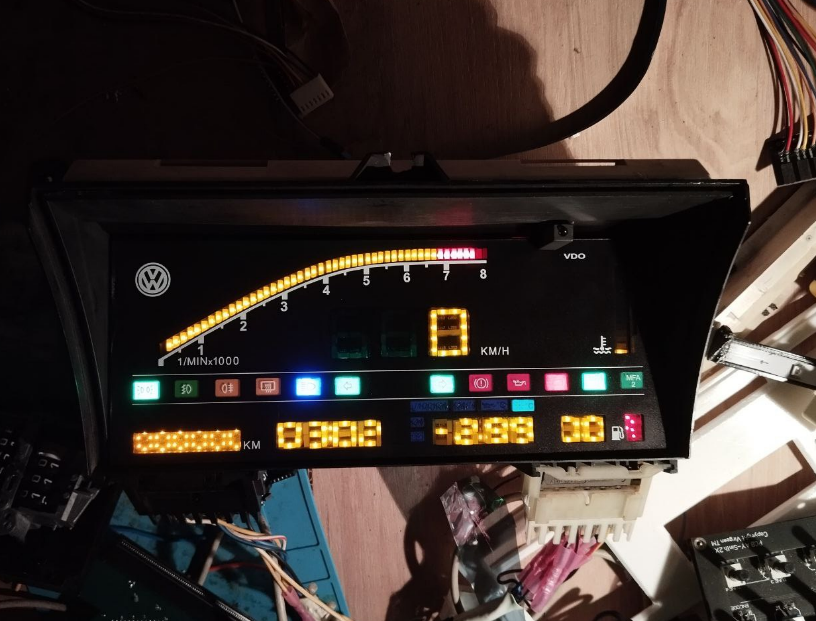
\includegraphics[width=\linewidth]{digifiz_manual/image046.png}
        \caption{\ReplicaGenOne{} classique avec encadrement carré.}
    \end{subfigure}\hfill
    \begin{subfigure}{0.46\textwidth}
        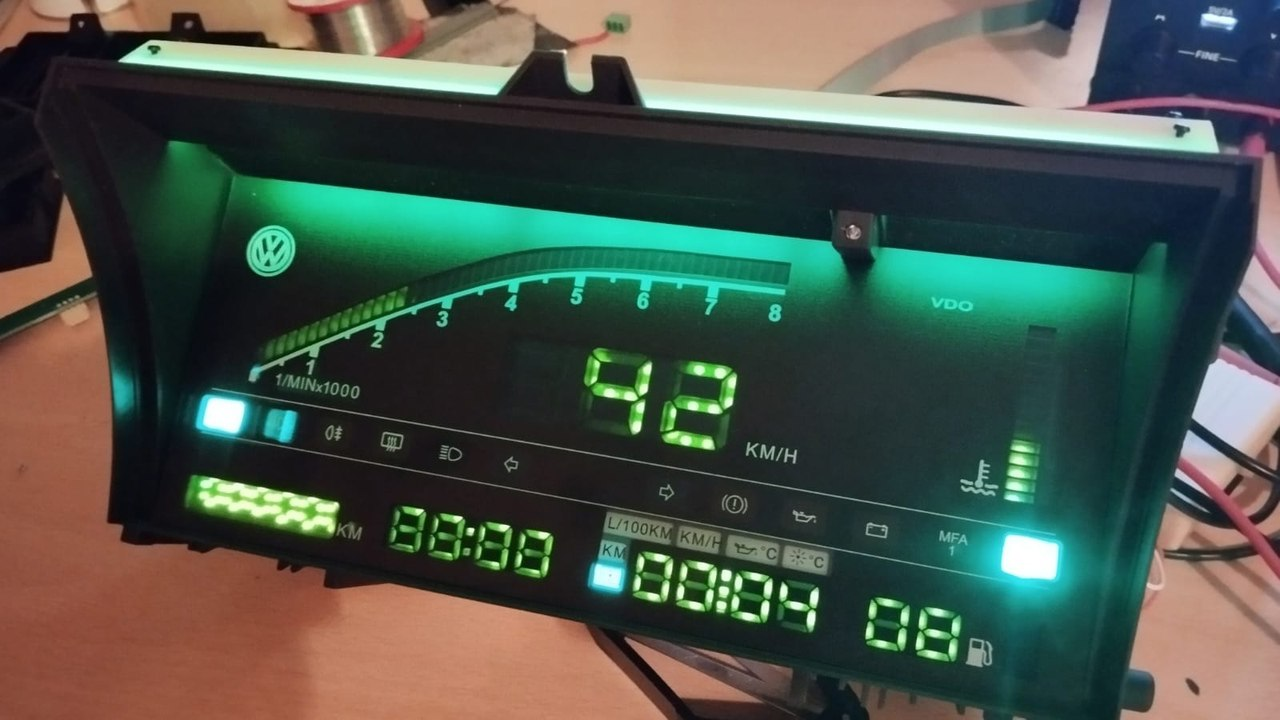
\includegraphics[width=\linewidth]{digifiz_manual/image047.png}
        \caption{Façade à angles arrondis utilisée sur les kits récents.}
    \end{subfigure}
    \caption{Aspect du tableau \ReplicaGenOne{}.}
    \label{fig:replica-classic}
\end{figure}

\section{Manipulation et entretien de l'écran}
\begin{itemize}
    \item La façade plexiglas imprimée aux UV se raye facilement. Évitez tout contact avec des objets pointus ou abrasifs.
    \item Les dommages de surface sont esthétiques et non couverts par la garantie. Demandez des pièces de rechange à PHOL-LABS Kft si le motif de l'écran est déformé.
\end{itemize}

\section{Pile de l'horloge temps réel}
Le tableau contient une horloge DS3231 alimentée par une pile CR2032 dont la durée de vie est d'environ quatre ans. Une fois déchargée, l'horloge se réinitialise à chaque mise sous tension. Retirez la façade et/ou le capot arrière, laissez les faisceaux branchés et remplacez la pile bouton. Éliminez la pile usagée conformément à la réglementation locale.

\section{Maintenance du micrologiciel avec USBasp}
Chaque kit est livré avec un cordon de programmation USBasp déjà connecté dans le boîtier (\autoref{fig:usbasp-cable}). Installez un pilote USBasp adapté avant le flashage, par exemple depuis l'adresse suivante~:
\displayurl{https://myrobot.ru/downloads/driver-usbasp-v-2.0-usb-isp-windows-7-8-10-xp.php}
Le programmateur alimente le tableau lorsqu'il est relié à un ordinateur, ce qui permet les essais sur établi.

\begin{figure}[htbp]
    \centering
    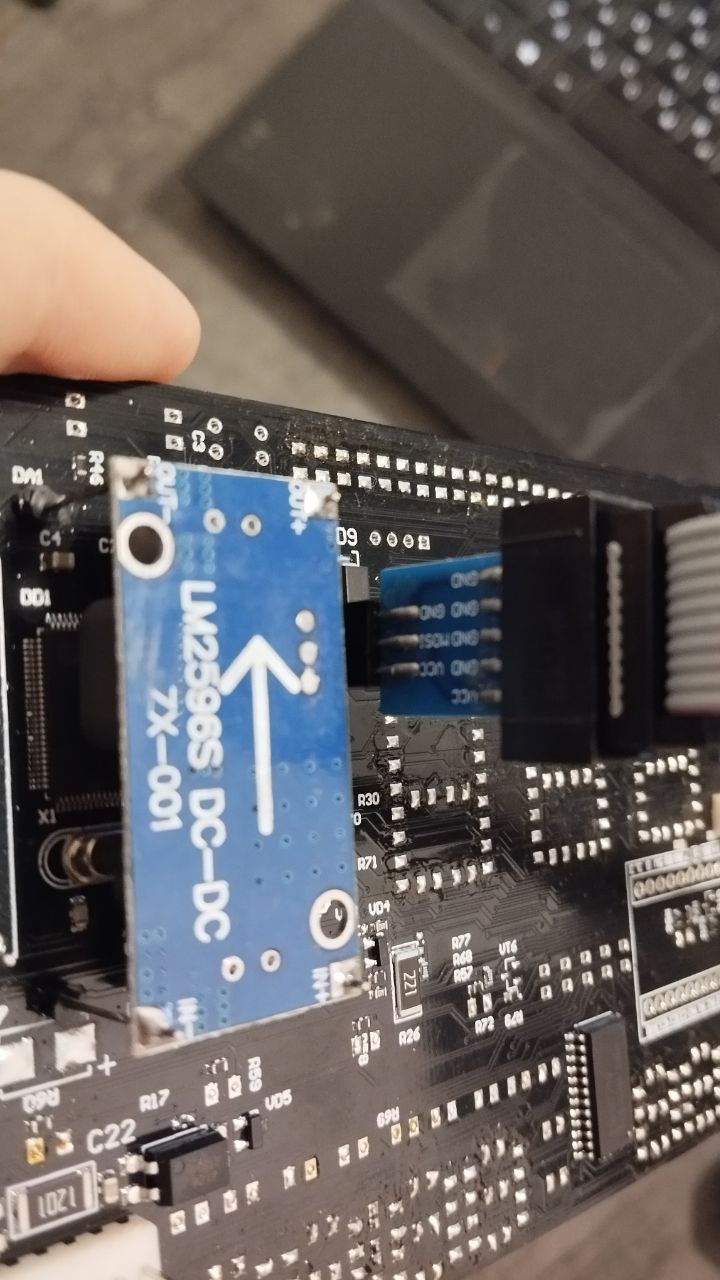
\includegraphics[width=0.32\textwidth]{digifiz_manual/image048.png}
    \caption{Orientation du faisceau USBasp dans \ReplicaGenOne{}.}
    \label{fig:usbasp-cable}
\end{figure}

Flashez le micrologiciel avec \texttt{avrdude} à l'aide de la commande ci-dessous (remplacez le nom du firmware si nécessaire)~:

\begin{verbatim}
avrdude -c usbasp -p m2560 -e \
    -U lfuse:w:0xff:m -U hfuse:w:0x99:m -U efuse:w:0xff:m \
    -U flash:w:Digifiz.ino.mega.hex
\end{verbatim}

Après un téléversement réussi, appuyez quatre à cinq fois sur le bouton tactile en façade pour initialiser les blocs mémoire. S'ils restent vides, répétez l'opération ou envoyez la commande Bluetooth \verb|252 0| pour lancer une réinitialisation usine. Des images prêtes à l'emploi sont publiées sur~:
\displayurl{https://github.com/Sgw32/DigifizReplica}

\section{Configuration Bluetooth}
La plupart des paramètres se règlent via Bluetooth depuis un téléphone Android avec l'application Serial Bluetooth Terminal. Téléchargez-la avant l'appairage~:
\displayurl{https://play.google.com/store/apps/details?id=de.kai_morich.serial_bluetooth_terminal&hl=en&gl=US}
Les appareils iOS ne peuvent pas se connecter au module Bluetooth 2.0 classique.

\begin{itemize}
    \item Associez-vous bien à l'interface Bluetooth Classic du tableau, et non à des périphériques BLE uniquement.
    \item Dans Serial Bluetooth Terminal, définissez le caractère de fin de ligne sur LF. Désactivez CR+LF avant d'envoyer des commandes.
\end{itemize}

\begin{figure}[htbp]
    \centering
    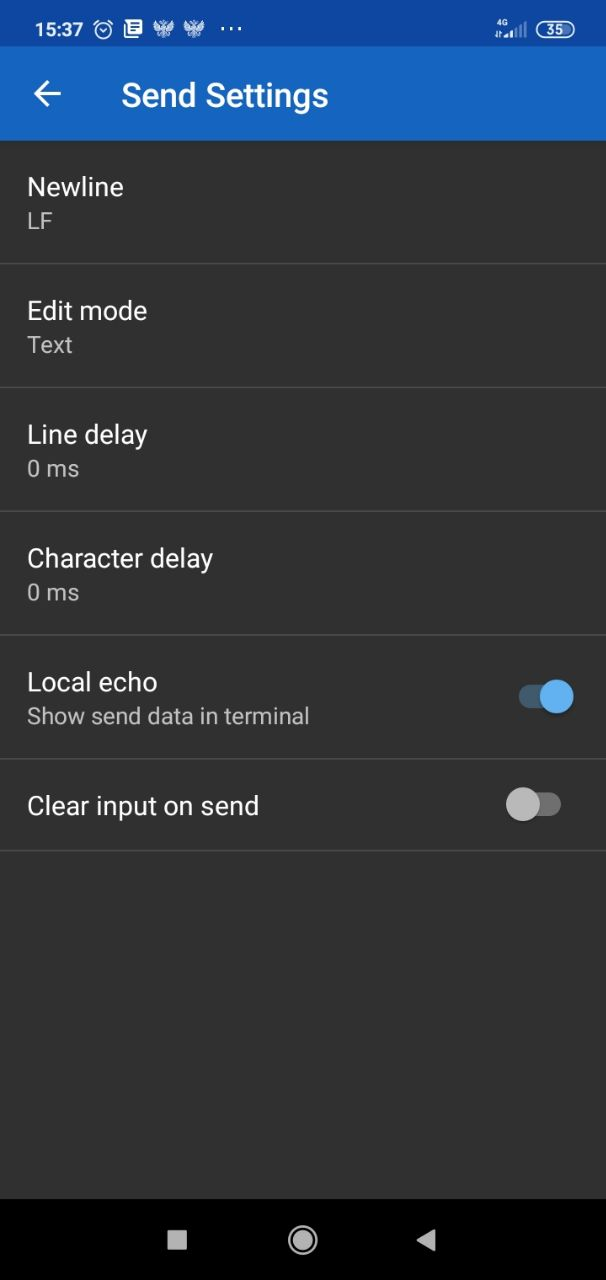
\includegraphics[width=0.32\textwidth]{digifiz_manual/image049.png}
    \caption{Configuration recommandée pour Serial Bluetooth Terminal.}
    \label{fig:sbt-settings}
\end{figure}

Saisissez les commandes sous forme de paires \verb|<nombre> <valeur>| séparées par un espace. Par exemple, pour enregistrer un odomètre de 123\,456~km, envoyez \verb|11 123456|. Ajoutez 128 au numéro d'une commande pour lire sa valeur actuelle (\verb|129 0| renvoie le coefficient de vitesse). La commande de diagnostic \verb|adc 0| affiche les lectures brutes utiles au diagnostic.

\section{Paramètres de configuration}
Les principales commandes Bluetooth figurent dans l'\autoref{tbl:replica-classic-commands}. Les paramètres par défaut des tableaux des générations~1/1.5 et~2 sont résumés à l'\autoref{tbl:replica-defaults}. N'utilisez les commandes~31--33 que sur \ReplicaNextShort{} ; elles n'ont aucun effet sur \ReplicaGenOneShort{} classique.

{\scriptsize
\begin{longtblr}[
    caption = {Commandes de configuration \ReplicaGenOne{} classique.},
    label = {tbl:replica-classic-commands},
]{
    colspec = {Q[c,0.14\linewidth] >{\ttfamily}Q[l,0.38\linewidth] Q[l]},
    rowsep = 2pt,
}
    \toprule
    \textbf{ID} & \textbf{Nom} & \textbf{Description} \\
    \midrule
    22 (ou 0) & PARAMETER\_RPMCOEFFICIENT & Facteur d'étalonnage du régime moteur. \\
    1 & PARAMETER\_SPEEDCOEFFICIENT & Facteur d'étalonnage de vitesse. \\
    2 & PARAMETER\_COOLANTTHERMISTORB & Coefficient bêta de thermistance liquide. \\
    3 & PARAMETER\_OILTHERMISTORB & Coefficient bêta de thermistance huile. \\
    4 & PARAMETER\_AIRTHERMISTORB & Coefficient bêta de thermistance ambiante. \\
    5 & PARAMETER\_TANKMINRESISTANCE & Résistance minimale de jauge (\si{\ohm}). \\
    6 & PARAMETER\_TANKMAXRESISTANCE & Résistance maximale de jauge (\si{\ohm}). \\
    7 & PARAMETER\_TAU\_COOLANT & Constante de filtrage température liquide. \\
    8 & PARAMETER\_TAU\_OIL & Constante de filtrage température huile. \\
    9 & PARAMETER\_TAU\_AIR & Constante de filtrage température ambiante. \\
    10 & PARAMETER\_TAU\_TANK & Constante de filtrage niveau carburant. \\
    11 & PARAMETER\_MILEAGE & Kilométrage total. \\
    12 & PARAMETER\_DAILY\_MILEAGE & Compteur journalier. \\
    13 & PARAMETER\_AUTO\_BRIGHTNESS & Activation du réglage automatique de luminosité. \\
    14 & PARAMETER\_BRIGHTNESS\_LEVEL & Niveau de luminosité manuel (0--15). \\
    15 & PARAMETER\_TANK\_CAPACITY & Capacité du réservoir (litres). \\
    16 & PARAMETER\_MFA\_STATE & Page MFA active. \\
    17 & PARAMETER\_BUZZER\_OFF & Désactivation du buzzer (1 coupe, 0 active). \\
    18 & PARAMETER\_MAX\_RPM & Échelle du compte-tours (8000 par défaut). \\
    19 & PARAMETER\_NORMAL\_RESISTANCE\_COOLANT & Résistance de sonde liquide à \SI{25}{\celsius}. \\
    20 & PARAMETER\_NORMAL\_RESISTANCE\_OIL & Résistance de sonde huile à \SI{25}{\celsius}. \\
    21 & PARAMETER\_NORMAL\_RESISTANCE\_AMB & Résistance de sonde ambiante à \SI{25}{\celsius}. \\
    23 & PARAMETER\_DOT\_OFF & Comportement des deux-points de l'horloge (0 clignote, 1 fixe). \\
    24 & PARAMETER\_BACKLIGHT\_ON & Allumage du rétroéclairage avec les feux de croisement. \\
    25 & PARAMETER\_M\_D\_FILTER & Constante de filtre médian (héritage). \\
    26 & PARAMETER\_COOLANT\_MAX\_R & Seuil pleine échelle de température liquide. \\
    27 & PARAMETER\_COOLANT\_MIN\_R & Seuil « 1~bar » de température liquide. \\
    31--33 & PARAMETER\_MAINCOLOR\_[RGB] & Composantes couleur interface (\ReplicaNextShort{} uniquement). \\
    37 & PARAMETER\_RPM\_FILTER & Agressivité du filtrage régime. \\
    128 & PARAMETER\_READ\_ADDITION & Addition pour lire un paramètre. \\
    255 & PARAMETER\_SET\_HOUR & Réglage des heures (24~h). \\
    254 & PARAMETER\_SET\_MINUTE & Réglage des minutes. \\
    253 & PARAMETER\_RESET\_DAILY\_MILEAGE & Remise à zéro du compteur journalier. \\
    252 & PARAMETER\_RESET\_DIGITAL & Réinitialisation usine et initialisation mémoire. \\
    \bottomrule
\end{longtblr}}

Les boutons rapides de Serial Bluetooth Terminal sont pratiques pour les actions courantes comme l'activation/désactivation de la luminosité automatique (\verb|13 0| et \verb|13 1|) ou l'écriture de valeurs de couleur. Ne dépassez \SI{60}{\percent} de luminosité que lors de tests courts afin de préserver les LED.

\chapter{Situations typiques lors du réglage de \ReplicaGenOne{}}\label{ch:replica-scenarios}

Avant tout dépannage, vérifiez que le tableau est bien un \ReplicaGenOne{} classique (\autoref{ch:replica-setup}). Les panneaux \ReplicaNextLong{} utilisent un portail Wi-Fi et sont traités au \autoref{ch:replica-next-scenarios}.

\begin{description}
    \item[Module Bluetooth introuvable] Associez-vous à l'interface Bluetooth Classic du tableau (il apparaît généralement comme \texttt{Digifiz}). Serial Bluetooth Terminal pour Android reste l'outil recommandé~: configurez le caractère de fin de ligne sur LF et évitez les scanners BLE uniquement, incapables de détecter le module.
    \item[iPhone ou iPad non compatible] Les tableaux \ReplicaGenOneShort{} emploient du Bluetooth~2.0 et sont incompatibles avec iOS. Utilisez un téléphone Android ou un ordinateur équipé d'un utilitaire série Bluetooth.
    \item[Commandes ignorées sur firmware 2024+] Déverrouillez l'analyseur de commandes en envoyant \verb|234 123|, puis rejouez la séquence souhaitée. Programmez des boutons rapides dans Serial Bluetooth Terminal pour les valeurs fréquemment ajustées.
    \item[Vitesse trop haute ou trop basse] Connectez-vous via Serial Bluetooth Terminal, roulez à \SI{100}{\kilo\metre\per\hour} indiqués et relevez la vitesse GPS. Envoyez \verb|1 <valeur_gps>| (par exemple \verb|1 85|) afin que \paramname{PARAMETER\_SPEEDCOEFFICIENT} corresponde à la vitesse vérifiée.
    \item[Régime erroné] Les micrologiciels antérieurs à 2024 attendent \verb|0 <valeur>| tandis que les versions actuelles utilisent \verb|22 <valeur>|. Les moteurs Audi nécessitent généralement \verb|22 3000| ; divisez ou doublez la valeur (par exemple \verb|22 1500| ou \verb|22 6000|) jusqu'à concordance avec le compte-tours.
    \item[Augmenter la luminosité] Désactivez le contrôle automatique avec \verb|13 0| puis augmentez le niveau manuel via \verb|14 <valeur>|. Des valeurs entre 45 et 55 éclairent nettement l'affichage ; évitez de dépasser 60 pour préserver les LED. Réactivez la photodiode ensuite avec \verb|13 1|.
    \item[Réglage de l'horloge] Utilisez Serial Bluetooth Terminal pour envoyer \verb|255 <heures>| puis \verb|254 <minutes>|. Exemples~: \verb|255 23|, \verb|254 55| règle 23:55 ; \verb|255 14|, \verb|254 30| règle 14:30 ; \verb|255 2|, \verb|254 28| règle 02:28.
    \item[Problèmes de jauge de carburant] Débranchez la batterie du véhicule avant toute mesure.\begin{itemize}
        \item Si l'affichage dérive de 60 vers 0, mesurez la résistance de la jauge entre la broche de faisceau et la masse ; les valeurs valides se situent généralement entre \SIrange{30}{300}{\ohm}. Nettoyez le connecteur et confirmez que le signal atteint la carte principale.
        \item Si la jauge reste au maximum, recherchez un court-circuit à la masse inférieur à \SI{5}{\ohm} sur la ligne de sonde et réparez-le.
        \item Si l'indication ne varie jamais, comparez la résistance de la jauge réservoir plein et vide. Remplacez le capteur s'il reste constant.
    \end{itemize}
    \item[Débit de carburant incohérent] Le canal de débit est simulé tant qu'aucun capteur de pression de collecteur n'est installé. Considérez la mesure comme indicative.
    \item[Jauge de liquide imprécise] Ajustez \paramname{PARAMETER\_COOLANT\_MIN\_R} et \paramname{PARAMETER\_COOLANT\_MAX\_R}. Exemple~: \verb|27 30| réduit l'échelle afin que la marque « 1~bar » corresponde à environ \SI{30}{\celsius}.
    \item[Température d'huile ou ambiante absente] Une valeur \texttt{-999} ou figée indique un souci de capteur. Batterie débranchée et moteur froid, mesurez la résistance entre la broche de faisceau et la masse. Les sondes d'huile doivent indiquer environ \SI{2}{\kilo\ohm} \ensuremath{\pm}\SI{0.3}{\kilo\ohm} ; les sondes ambiantes environ \SI{10}{\kilo\ohm} \ensuremath{\pm}\SI{2}{\kilo\ohm}. Ajustez \paramname{PARAMETER\_NORMAL\_RESISTANCE\_OIL} (commande~20) ou \paramname{PARAMETER\_NORMAL\_RESISTANCE\_AMB} (commande~21) si l'affichage nécessite un calibrage fin. En cas de panne persistante, consignez les relevés \verb|adc 0| et transmettez-les au support PHOL-LABS Kft.
\end{description}

Collectez les données brutes des capteurs avec \verb|adc 0| si le problème perdure et communiquez les résultats aux développeurs pour analyse.

\chapter{Marquage et scellés}\label{ch:marking}

\begin{itemize}
    \item Chaque tableau peut recevoir le numéro de modèle correspondant à sa variante de combiné.
    \item Les lots destinés à l'export peuvent comporter des marquages supplémentaires apposés par l'organisme importateur.
    \item \ReplicaGenOne{} n'est pas scellé ; aucun autocollant inviolable n'est posé en usine.
\end{itemize}

\chapter{Emballage}\label{ch:package}

\begin{enumerate}
    \item Pour le transport, enveloppez le tableau et ses accessoires dans du papier bulle puis placez l'ensemble dans une boîte en carton rigide.
    \item Tout autre conditionnement est acceptable dès lors qu'il protège le combiné pendant le transport et le stockage.
\end{enumerate}

\chapter{Règles de stockage et de transport}\label{ch:storage}

\begin{itemize}
    \item Les conditions de transport doivent respecter les règles générales de fret propres à chaque mode (GOST~23216-78).
    \item Les tableaux emballés peuvent voyager par route, rail, voie fluviale ou aérienne.
    \item Stockez le combiné dans l'habitacle du véhicule ou dans un local chauffé entre \SI{15}{\celsius} et \SI{40}{\celsius}. Protégez l'appareil de la lumière directe du soleil, même si le stockage derrière une vitre de véhicule reste acceptable.
\end{itemize}


\appendix
\chapter{Tableaux de référence} \label{appendix:reference}

\section{Référence des commandes \ReplicaGenOne{} classique}

Le micrologiciel Replica classique partage la plupart des commandes avec \ReplicaNextShort{}.
Les commandes 31--33 (contrôle des couleurs) ne sont actives que sur \ReplicaNextShort{} ; les autres s'appliquent aux deux générations.

\begin{table}[htbp]
    \centering
    \caption{Principales commandes de configuration pour les tableaux \ReplicaGenOne{} classiques.}
    \label{tbl:replica-commands}
    {\scriptsize
    \begin{tblr}{
        colspec = {>{\ttfamily}Q[c,0.12\linewidth] Q[l] Q[l]},
        rowsep = 2pt,
    }
        \toprule
        \textbf{Commande} & \textbf{Nom} & \textbf{Description} \\
        \midrule
        22 (ou 0) & PARAMETER\_RPMCOEFFICIENT & Facteur d'étalonnage du régime moteur. \\
        1  & PARAMETER\_SPEEDCOEFFICIENT & Facteur d'étalonnage de vitesse. \\
        2  & PARAMETER\_COOLANTTHERMISTORB & Coefficient bêta de la thermistance liquide. \\
        3  & PARAMETER\_OILTHERMISTORB & Coefficient bêta de la thermistance d'huile. \\
        4  & PARAMETER\_AIRTHERMISTORB & Coefficient bêta de la thermistance ambiante. \\
        5  & PARAMETER\_TANKMINRESISTANCE & Résistance minimale de jauge. \\
        6  & PARAMETER\_TANKMAXRESISTANCE & Résistance maximale de jauge. \\
        7--10 & PARAMETER\_TAU\_\textit{X} & Constantes de filtrage pour le liquide, l'huile, l'air et le niveau de carburant. \\
        11 & PARAMETER\_MILEAGE & Kilométrage total. \\
        12 & PARAMETER\_DAILY\_MILEAGE & Compteur journalier. \\
        13 & PARAMETER\_AUTO\_BRIGHTNESS & Activation de la luminosité automatique. \\
        14 & PARAMETER\_BRIGHTNESS\_LEVEL & Niveau de luminosité manuel. \\
        15 & PARAMETER\_TANK\_CAPACITY & Capacité du réservoir. \\
        16 & PARAMETER\_MFA\_STATE & Mode MFA actif. \\
        17 & PARAMETER\_BUZZER\_OFF & Désactivation du buzzer (Replica uniquement). \\
        18 & PARAMETER\_MAX\_RPM & Échelle du compte-tours (7000 par défaut). \\
        19--21 & PARAMETER\_NORMAL\_RESISTANCE\_\textit{X} & Résistances de capteurs à \SI{25}{\celsius} pour liquide, huile et air. \\
        23 & PARAMETER\_DOT\_OFF & Comportement des deux-points de l'horloge. \\
        24 & PARAMETER\_BACKLIGHT\_ON & Activation du rétroéclairage avec les feux de croisement. \\
        25 & PARAMETER\_M\_D\_FILTER & Constante de filtre médian. \\
        26 & PARAMETER\_COOLANT\_MAX\_R & Seuil de sonde liquide pour affichage pleine échelle. \\
        27 & PARAMETER\_COOLANT\_MIN\_R & Seuil de sonde liquide pour l'indication « 1~bar ». \\
        31--33 & PARAMETER\_MAINCOLOR\_[RGB] & Composantes de couleur de l'interface (\ReplicaNextShort{} uniquement). \\
        37 & PARAMETER\_RPM\_FILTER & Agressivité du filtrage régime. \\
        128 & PARAMETER\_READ\_ADDITION & Ajouter 128 pour lire la valeur courante d'une commande. \\
        255 & PARAMETER\_SET\_HOUR & Réglage des heures. \\
        254 & PARAMETER\_SET\_MINUTE & Réglage des minutes. \\
        253 & PARAMETER\_RESET\_DAILY\_MILEAGE & Remise à zéro du compteur journalier. \\
        252 & PARAMETER\_RESET\_DIGITAL & Réinitialisation usine des paramètres stockés. \\
        \bottomrule
    \end{tblr}}
\end{table}

\section{Valeurs par défaut \ReplicaGenOneShort{} classique}

\begin{table}[htbp]
    \centering
    \caption{Configuration par défaut du \ReplicaGenOne{} classique.}
    \label{tbl:replica-defaults}
    {\scriptsize
    \begin{tblr}{
        colspec = {>{\ttfamily}Q[c,0.22\linewidth] Q[c,0.16\linewidth] Q[l]},
        rowsep = 2pt,
    }
        \toprule
        \textbf{Paramètre} & \textbf{Valeur} & \textbf{Remarques} \\
        \midrule
        PARAMETER\_RPMCOEFFICIENT & 3000 &  \\
        PARAMETER\_SPEEDCOEFFICIENT & 100 &  \\
        PARAMETER\_COOLANTTHERMISTORB & 4000 &  \\
        PARAMETER\_OILTHERMISTORB & 4000 &  \\
        PARAMETER\_AIRTHERMISTORB & 3812 & 3600 sur Gen~2. \\
        PARAMETER\_TANKMINRESISTANCE & 35 & Ohms. \\
        PARAMETER\_TANKMAXRESISTANCE & 265 & Ohms. \\
        PARAMETER\_TAU\_COOLANT & 2 &  \\
        PARAMETER\_TAU\_OIL & 2 &  \\
        PARAMETER\_TAU\_AIR & 2 &  \\
        PARAMETER\_TAU\_TANK & 2 &  \\
        PARAMETER\_MILEAGE & Spécifique au véhicule & Conserve l'odomètre existant. \\
        PARAMETER\_DAILY\_MILEAGE & 0 &  \\
        PARAMETER\_AUTO\_BRIGHTNESS & 1 & Activée. \\
        PARAMETER\_BRIGHTNESS\_LEVEL & 7 ou 13 & Valeurs typiques pour Gen~1/1.5. \\
        PARAMETER\_TANK\_CAPACITY & 63 & Litres. \\
        PARAMETER\_MFA\_STATE & 0 &  \\
        PARAMETER\_BUZZER\_OFF & 1 & Buzzer désactivé. \\
        PARAMETER\_MAX\_RPM & 8000 & 7000 sur les blocs plus anciens. \\
        PARAMETER\_NORMAL\_RESISTANCE\_COOLANT & 1000 & \si{\ohm} à \SI{25}{\celsius}. \\
        PARAMETER\_NORMAL\_RESISTANCE\_OIL & 1000 & \si{\ohm} à \SI{25}{\celsius}. \\
        PARAMETER\_NORMAL\_RESISTANCE\_AMB & 2991 & \si{\ohm} à \SI{25}{\celsius}. \\
        PARAMETER\_DOT\_OFF & 0 & Deux-points clignotant. \\
        PARAMETER\_BACKLIGHT\_ON & 1 & Activé. \\
        PARAMETER\_M\_D\_FILTER & 65535 &  \\
        PARAMETER\_COOLANT\_MAX\_R & 120 & \si{\celsius}. \\
        PARAMETER\_COOLANT\_MIN\_R & 60 & \si{\celsius}. \\
        PARAMETER\_MAINCOLOR\_[RGB] & -- & Commandes couleur inactives sur Replica classique. \\
        PARAMETER\_RPM\_FILTER & 70 &  \\
        PARAMETER\_UPTIME & 0 &  \\
        \bottomrule
    \end{tblr}}
\end{table}

\section{Historique des révisions} \label{app:change-log}

\begin{table}[htbp]
    \centering
    \caption{Feuille d'enregistrement des modifications.}
    \label{tbl:change-log}
    {\scriptsize
    \begin{tblr}{
        colspec = {Q[c,0.12\linewidth] Q[l] Q[c,0.2\linewidth]},
        rowsep = 2pt,
    }
        \toprule
        \textbf{Modification} & \textbf{Feuilles affectées} & \textbf{Date} \\
        \midrule
        1 & 04.10.2022 & 04~oct.~2022 \\
        2 & 31.08.2023 & 31~août~2023 \\
        3 & 05.08.2024 & 05~août~2024 \\
        4 & Document LaTeX introduit. & 22.09.2025 \\
        \bottomrule
    \end{tblr}}
\end{table}


\backmatter
\references

\end{document}
